In this section, we study the discrimination of a boosted hadronically decaying $W$ signal against a gluon
background, comparing the performance of various groomed jet
masses, substructure variables, and BDT combinations of groomed mass
and substructure. We produce ROC
curves that elucidate the performance of the various groomed mass and
substructure variables. A
range of different distance parameters $R$ for the \antikt~jet
algorithm are explored, as well as a variety of kinematic regimes
(lead jet \pt 300-400 GeV, 500-600 GeV, 1.0-1.1 TeV). This allows us to determine the
performance of observables as a function of jet radius and jet boost, and to see
where different approaches may break down. The groomed
mass and substructure variables are then combined in a BDT as described in Section~\ref{sec:multivariate}, and the performance of the resulting BDT discriminant
explored through ROC curves to understand the degree to which
variables are correlated, and how
this changes with jet boost and jet radius. 

\subsection{Methodology}

These studies use the $WW$ samples as signal and the dijet $gg$ as background, described previously in Section~\ref{sec:samples}. Whilst only gluonic backgrounds
are explored here, the conclusions as to the dependence of the
performance and correlations on the jet boost and radius have been
verified to hold also for $qq$ backgrounds. {\bf ED: To be checked!}

As in the q/g tagging studies, the showered events were clustered with \textsc{FastJet}
3.03 using
the \antikt~algorithm with jet radii of $R = 0.4,\, 0.8,\, 1.2$. In
both signal and background samples, an upper and lower cut on
the leading jet $\pt$ is applied after showering/clustering, to ensure
similar $\pt$ spectra for signal and background in each \pt bin. The bins
in leading jet \pt that are considered are 300-400 GeV, 500-600 GeV,
1.0-1.1 TeV, for the 300-400 GeV, 500-600 GeV,
1.0-1.1 TeV parton \pt slices respectively. The jets then have various
grooming approaches applied and substructure observables
reconstructed as described in
Section~\ref{sec:observables}. 
{\bf (ED: Better if some of the information from
  Section~\ref{sec:observables} is brought into
  this section to avoid this back-referencing?)}

% and have various
%jet grooming approaches applied as described in Section~\ref{sec:substructure}. The following event selection is then applied to these
%samples....(presumably this will vary depending on which kinematic bin
%is used, as will the actual samples used - maybe summarize in a table).
%
%Figure~\ref{fig:pt300_basics} shows a comparison of the
%leading jet \pt for the signal and background in the \pt 300-400 GeV bin, for the two different \antikt jet
%algorithm distance parameters explored in this bin (R=0.8 and R=1.2). Figures~\ref{fig:pt500_basics} and~\ref{fig:pt1000_basics}  show the same for the
%\pt = 500-600 GeV bin and \pt = 1.0-1.1 TeV bin respectively, where for
%the \pt = 1.0-1.1 TeV bin the distance parameter R=0.4 is also explored because the W radiation at this boost is typically confined to 
%a cone of this size.
%
%
%
%\begin{figure*}
%\begin{center}
%\subfigure[\antikt R=0.8]{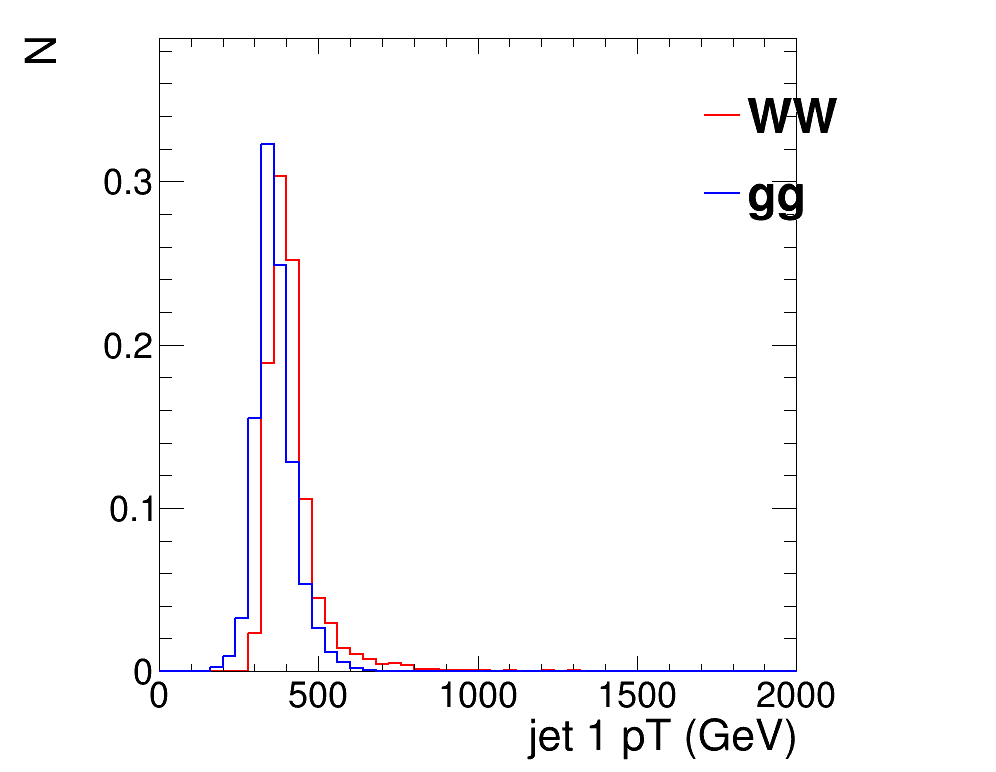
\includegraphics[width=0.30\textwidth]{./Figures/WTagging/pT300/AKtR08/jpt1.png}}
%\subfigure[\antikt R=1.2]{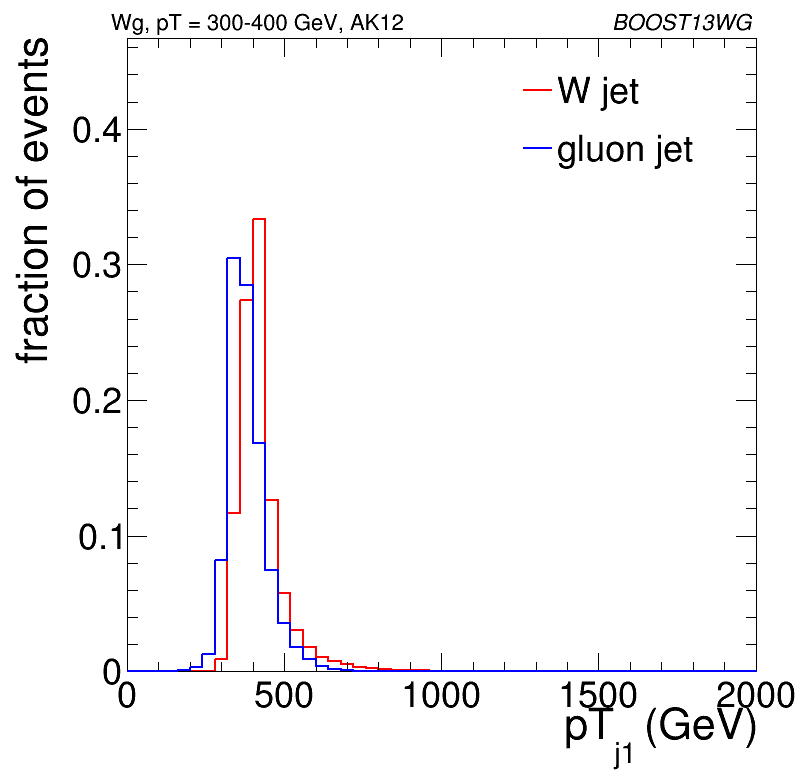
\includegraphics[width=0.30\textwidth]{./Figures/WTagging/pT300/AKtR12/jpt1.png}}
%\caption{Comparisons of the leading jet \pt spectrum of the $gg$
%  background to the WW signal in the \pt 300-400 GeV bin using the
%  different \antikt jet distance parameters explored.}
%\label{fig:pt300_basics}
%\end{center}
%\end{figure*}
%
%\begin{figure*}
%\begin{center}
%\subfigure[\antikt R=0.8]{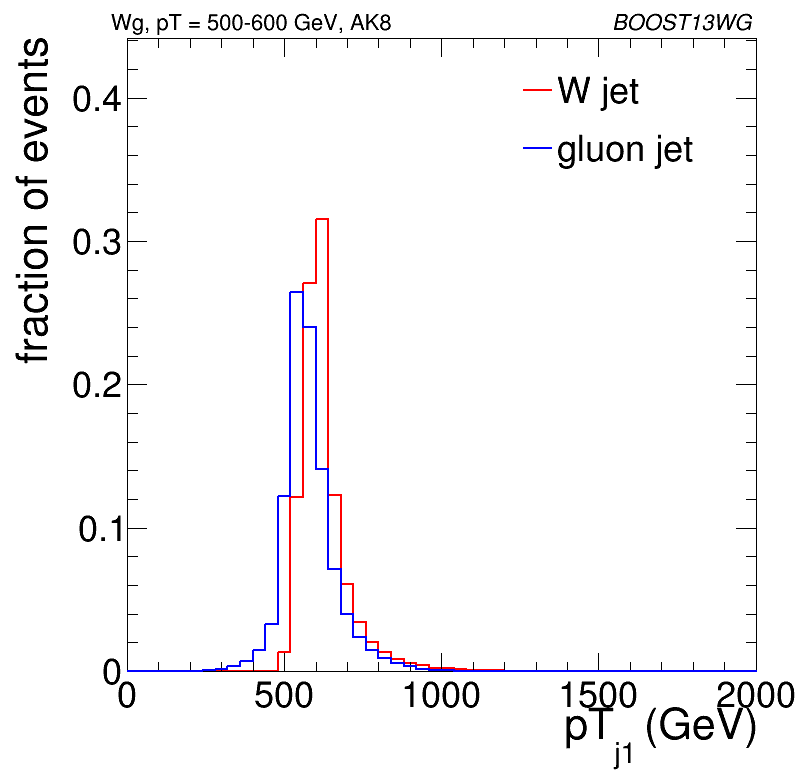
\includegraphics[width=0.30\textwidth]{./Figures/WTagging/pT500/AKtR08/jpt1.png}}
%\subfigure[\antikt R=1.2]{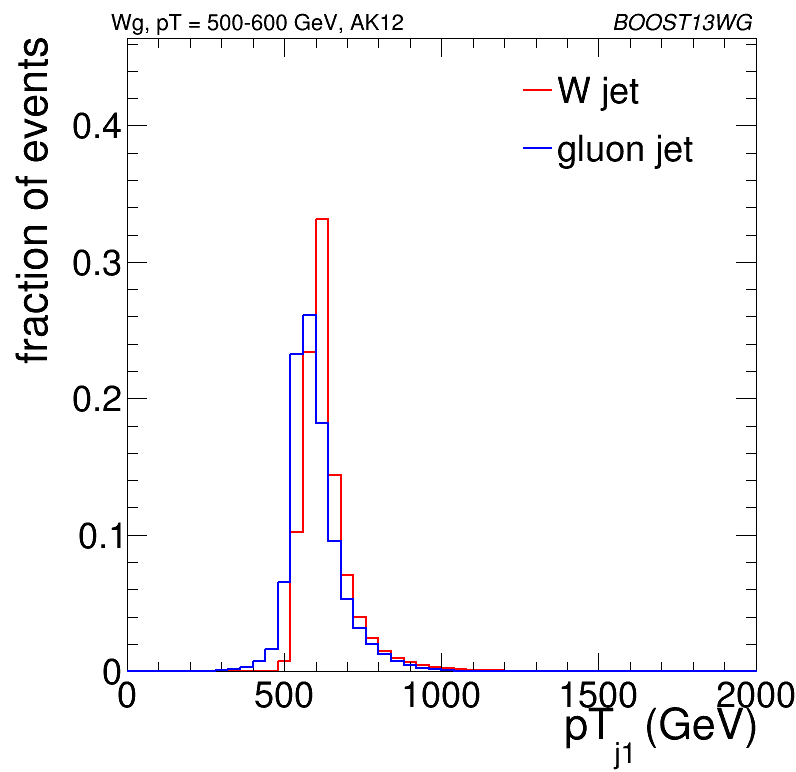
\includegraphics[width=0.30\textwidth]{./Figures/WTagging/pT500/AKtR12/jpt1.png}}
%\caption{Comparisons of the leading jet \pt spectrum of the $gg$
%  background to the WW signal in the \pt 500-600 GeV bin using the
%  different \antikt jet distance parameters explored.}
%\label{fig:pt500_basics}
%\end{center}
%\end{figure*}
%
%\begin{figure*}
%\begin{center}
%\subfigure[\antikt R=0.4]{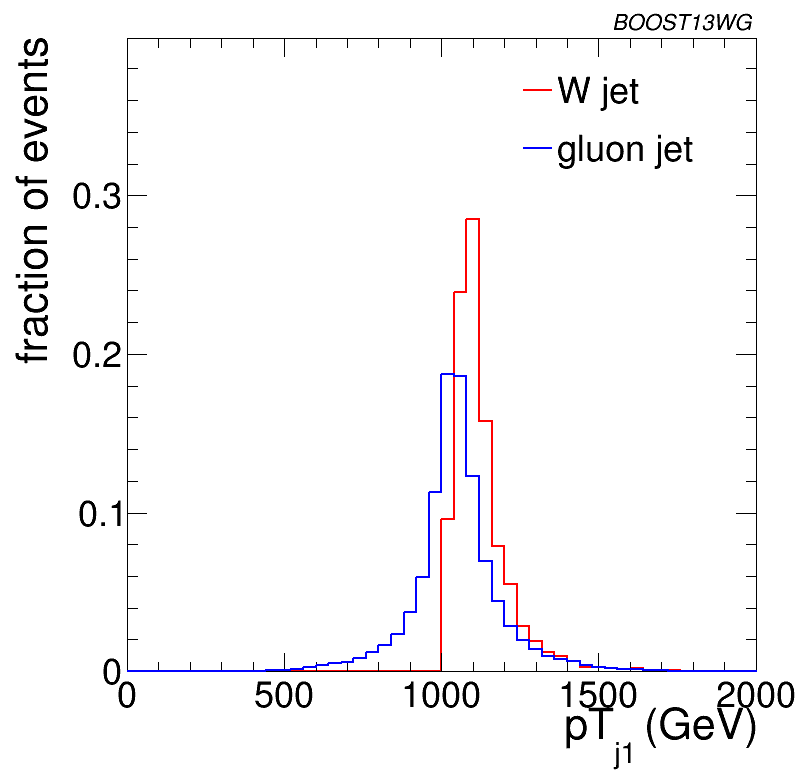
\includegraphics[width=0.30\textwidth]{./Figures/WTagging/pT1000/AKtR04/jpt1.png}}
%\subfigure[\antikt R=0.8]{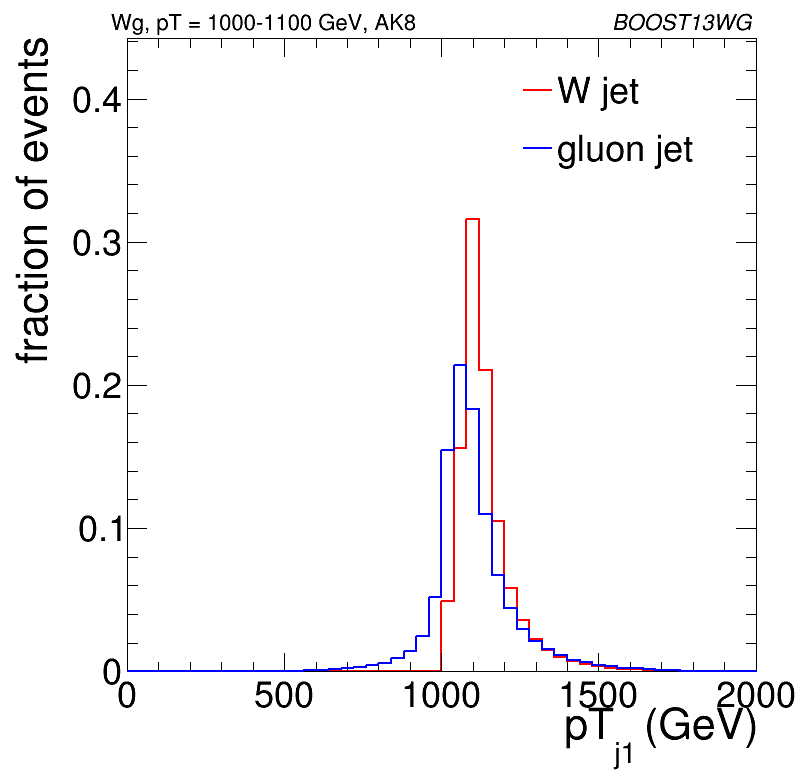
\includegraphics[width=0.30\textwidth]{./Figures/WTagging/pT1000/AKtR08/jpt1.png}}
%\subfigure[\antikt R=1.2]{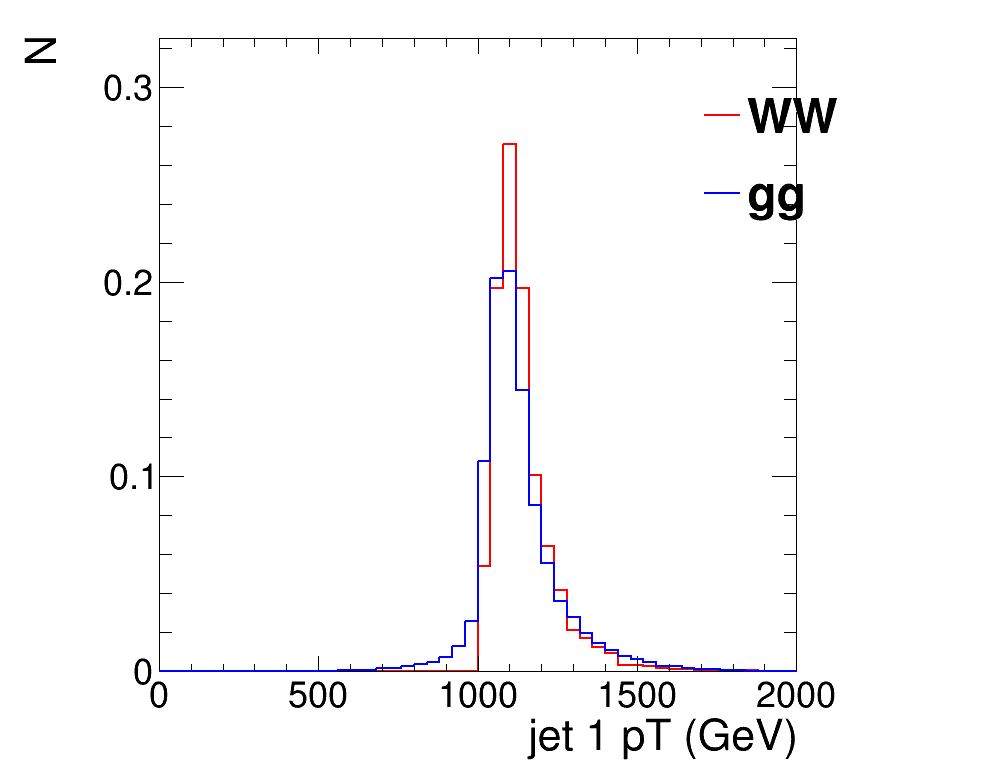
\includegraphics[width=0.30\textwidth]{./Figures/WTagging/pT1000/AKtR12/jpt1.png}}
%\caption{Comparisons of the leading jet \pt spectrum of the $gg$
%  background to the WW signal in the \pt 1.0-1.1 TeV bin using the
%  different \antikt jet distance parameters explored.}
%\label{fig:pt1000_basics}
%\end{center}
%\end{figure*}



\subsection{Single Variable Performance}

In this section we will explore the performance of the various groomed
jet mass and substructure variables in terms of discriminating signal
and background, and how this performance changes depending on the
kinematic bin and jet radius considered.

Figure~\ref{fig:pt500_mass_AKt_R08} the compares the signal and
background in terms of the different groomed masses explored for the
\antikt R=0.8 algorithm in the \pt 500-600 bin. One can clearly see
that in terms of separating signal and background the groomed masses
will be significantly more performant than the ungroomed \antikt R=0.8
mass.
Figure~\ref{fig:pt500_subst_AKt_R08}
compares signal and background in the different substructure variables
explored for the same jet radius and kinematic bin. 

\begin{figure*}
\begin{center}
\subfigure[Ungroomed mass]{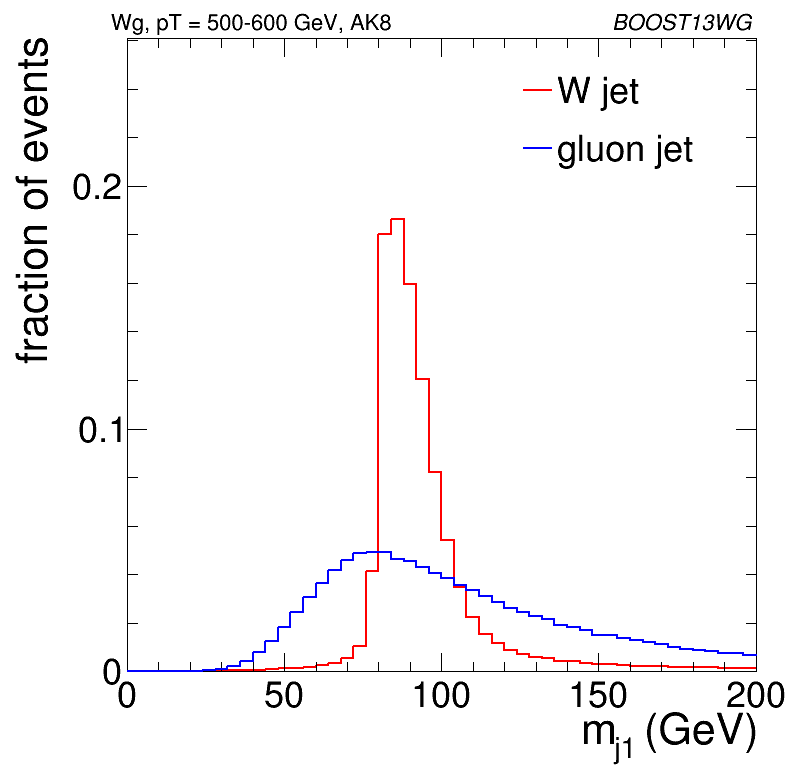
\includegraphics[width=0.30\textwidth]{./Figures/WTagging/pT500/AKtR08/jmass1.png}}
\subfigure[Pruned mass]{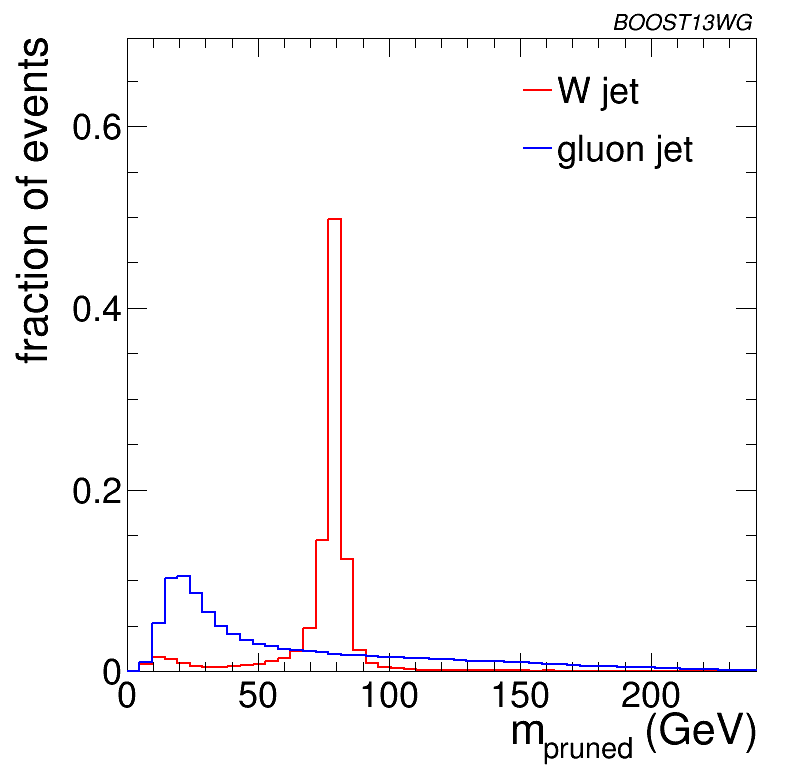
\includegraphics[width=0.30\textwidth]{./Figures/WTagging/pT500/AKtR08/h_mass_prun.png}}
\subfigure[Trimmed mass]{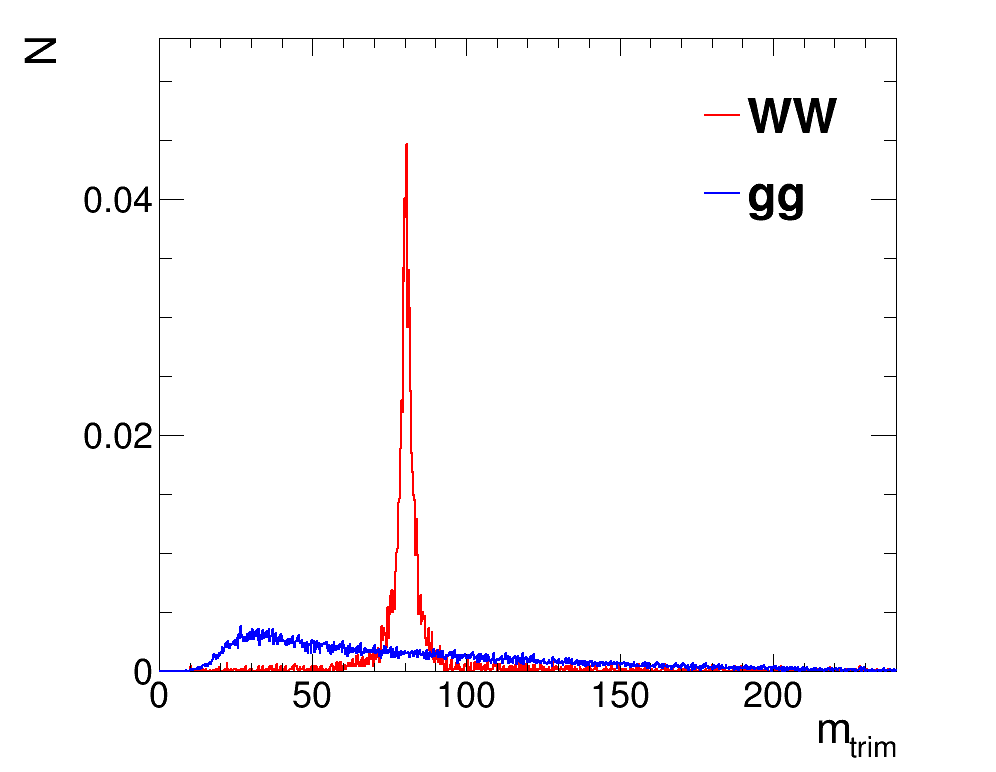
\includegraphics[width=0.30\textwidth]{./Figures/WTagging/pT500/AKtR08/h_mass_trim.png}}\\
\subfigure[mMDT mass]{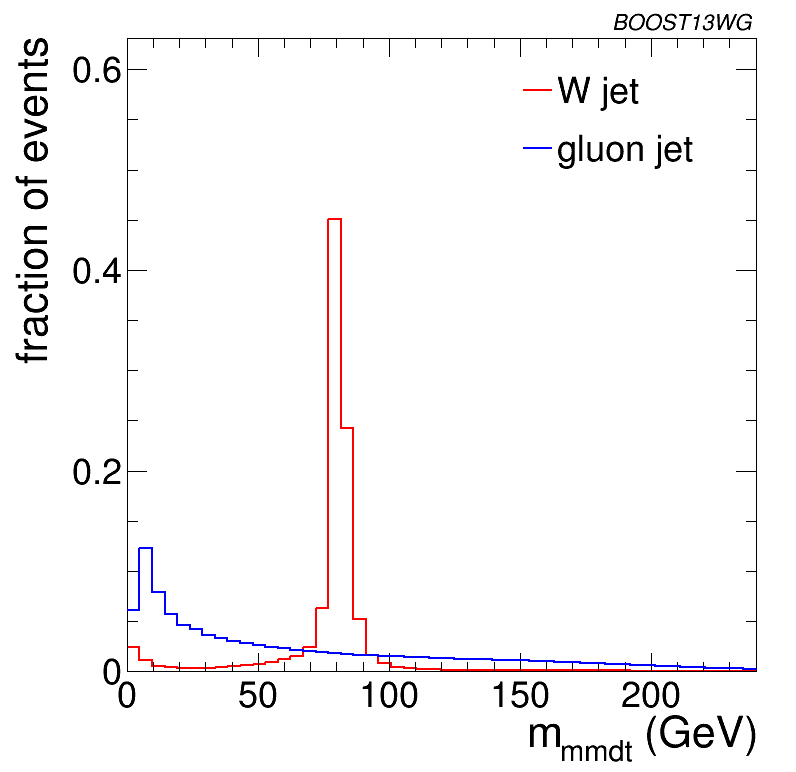
\includegraphics[width=0.30\textwidth]{./Figures/WTagging/pT500/AKtR08/h_mass_mmdt.png}}
\subfigure[Soft-drop $\beta=2$ mass]{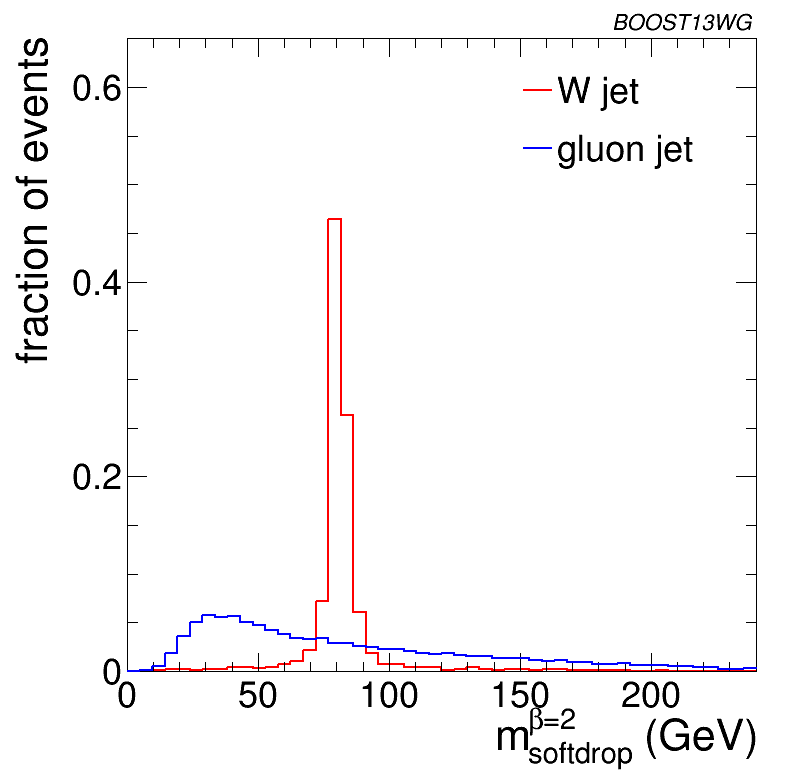
\includegraphics[width=0.30\textwidth]{./Figures/WTagging/pT500/AKtR08/h_mass_sdb2.png}}
%\subfigure[Soft-drop $\beta=-1$ mass]{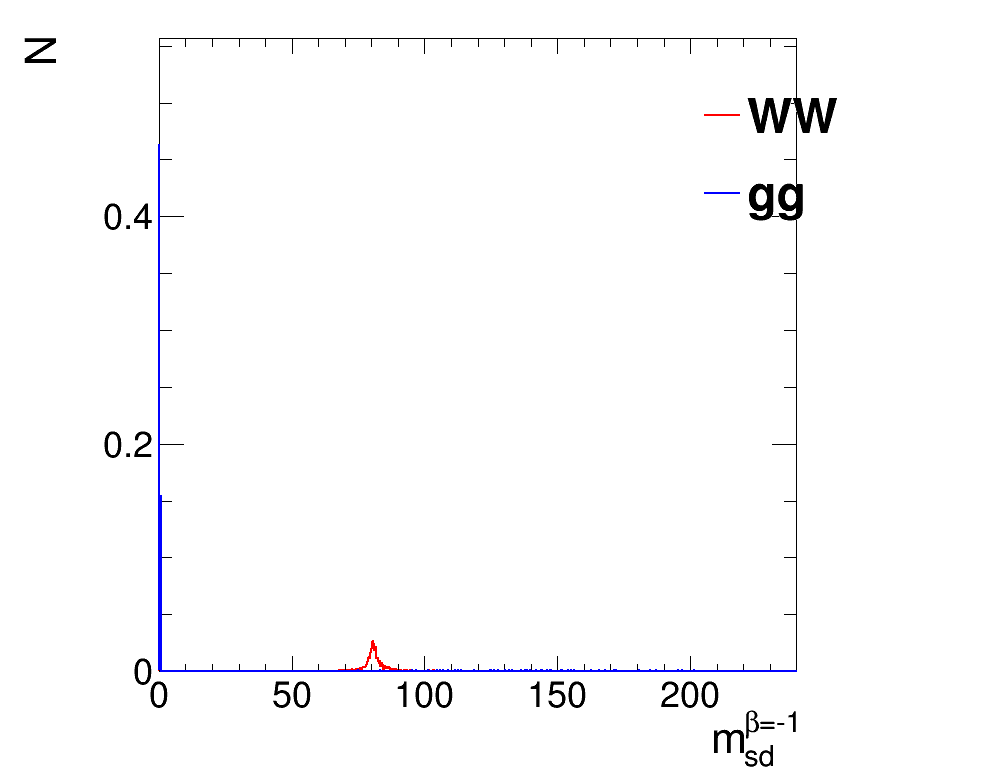
\includegraphics[width=0.48\textwidth]{./Figures/figs072514/figs071614_Wg_bin500_ak08/oneD/h_mass_sdm1.png}}
\caption{Comparisons of the QCD background to the WW signal in the \pt 500-600 GeV bin using the anti-\kT R=0.8 algorithm: leading
 jet mass distributions.}
\label{fig:pt500_mass_AKt_R08}
\end{center}
\end{figure*}

\begin{figure*}
\begin{center}
\subfigure[$C_2^{\beta=1}$]{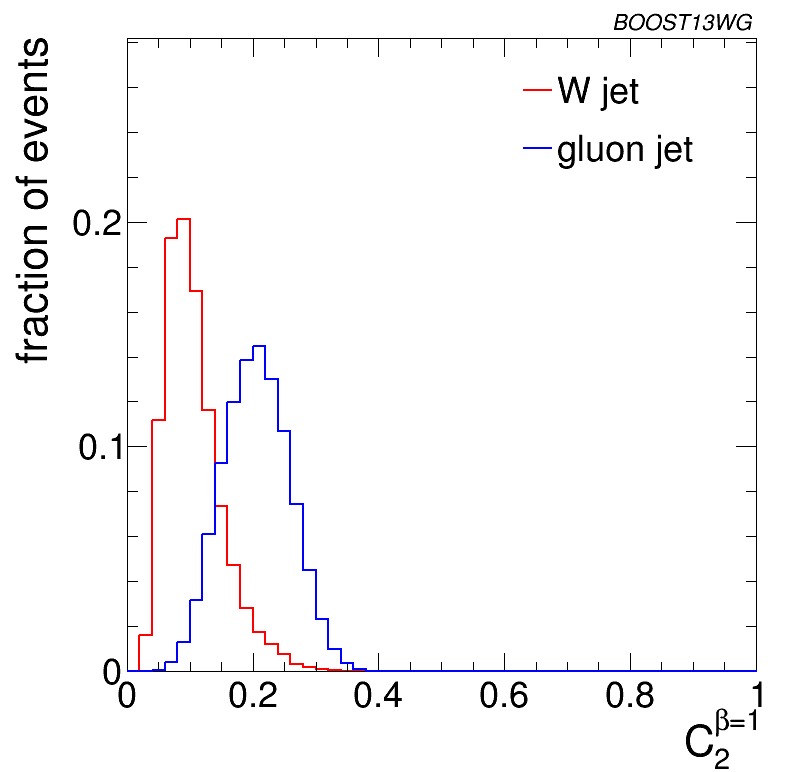
\includegraphics[width=0.30\textwidth]{./Figures/WTagging/pT500/AKtR08/h_c2_b1.png}}
\subfigure[$C_2^{\beta=2}$]{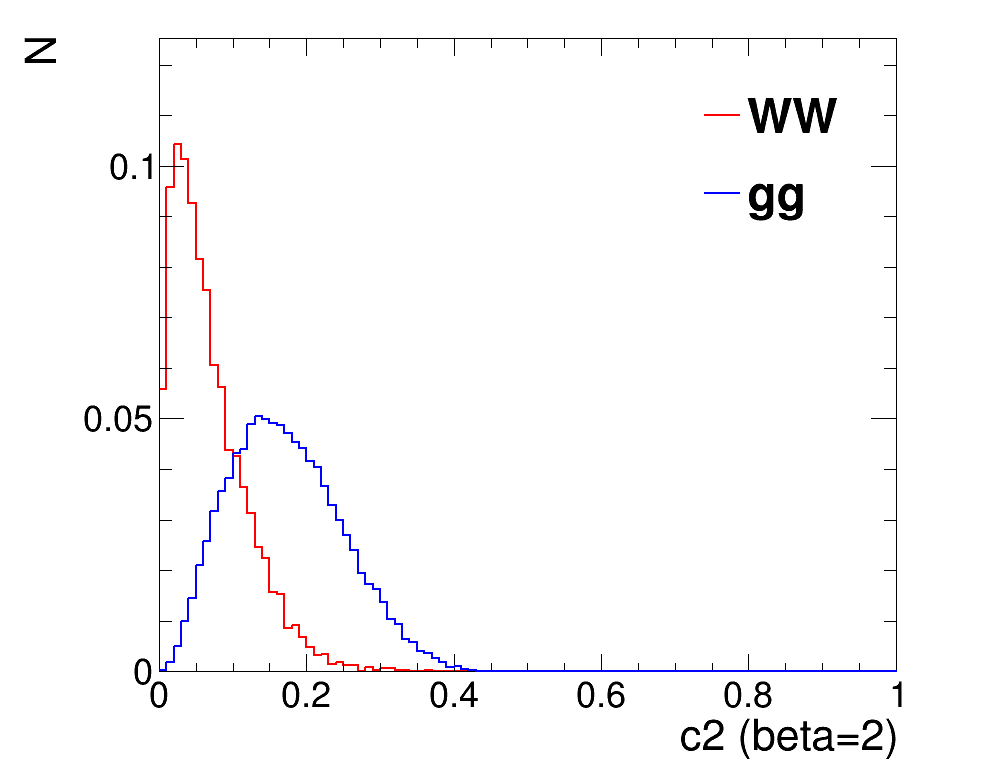
\includegraphics[width=0.30\textwidth]{./Figures/WTagging/pT500/AKtR08/h_c2_b2.png}}
\subfigure[$\Gamma_{Qjet}$]{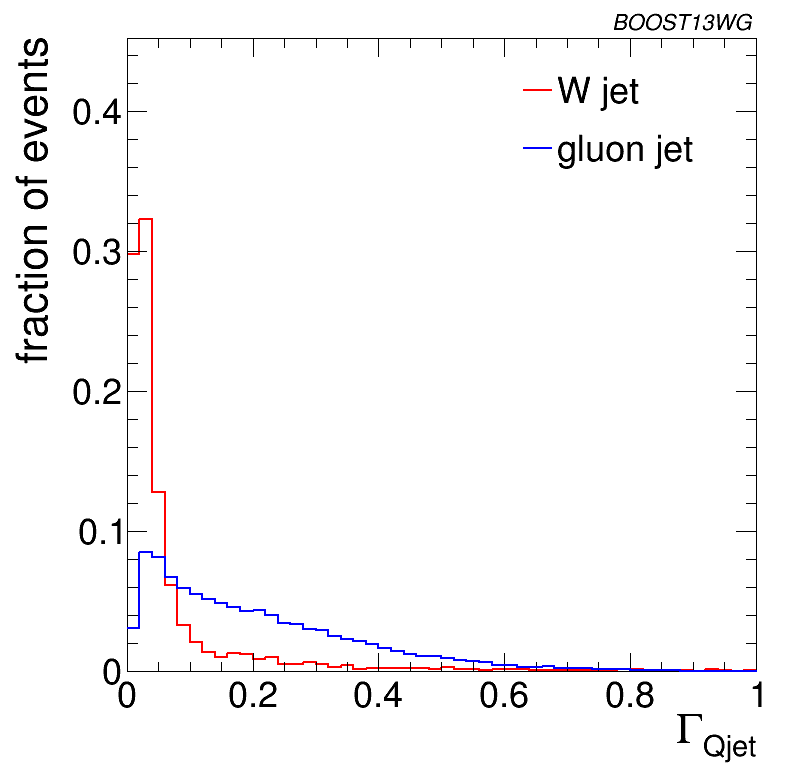
\includegraphics[width=0.30\textwidth]{./Figures/WTagging/pT500/AKtR08/h_qjetVol.png}}\\
\subfigure[$\tau_{21}^{\beta=1}$]{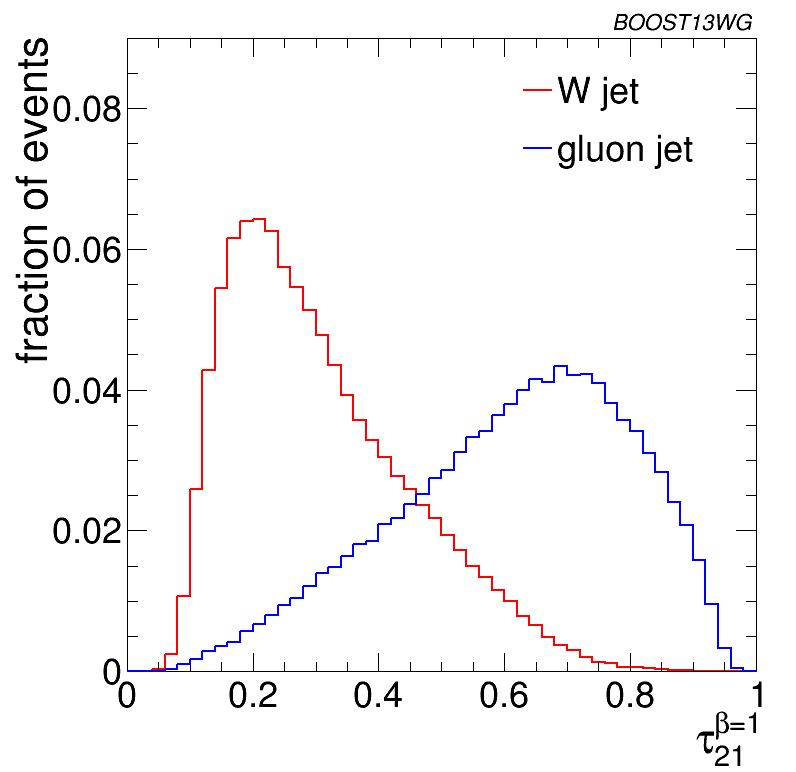
\includegraphics[width=0.30\textwidth]{./Figures/WTagging/pT500/AKtR08/h_tau21_b1.png}}
\subfigure[$\tau_{21}^{\beta=2}$]{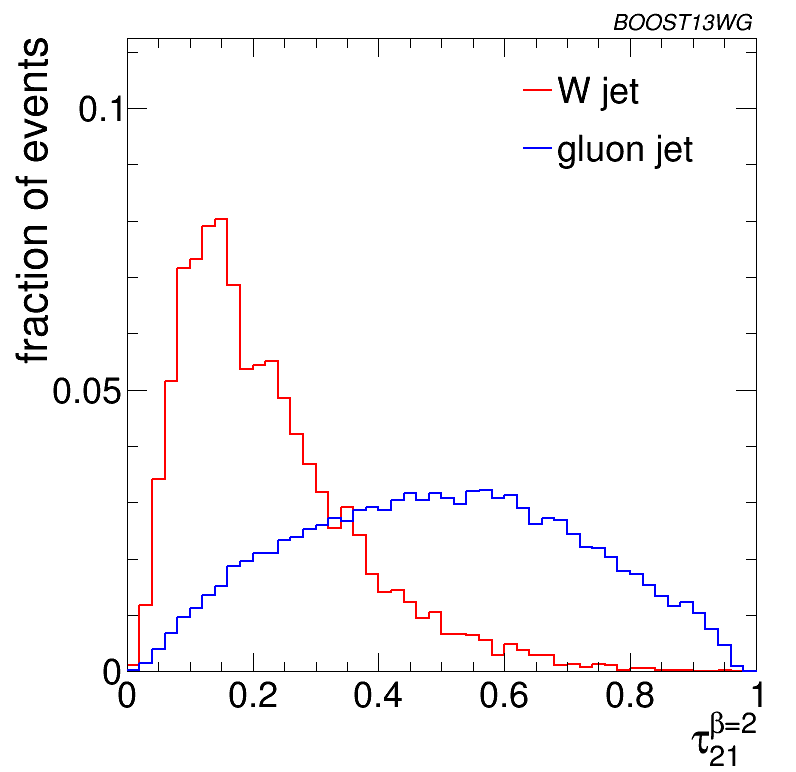
\includegraphics[width=0.30\textwidth]{./Figures/WTagging/pT500/AKtR08/h_tau21_b2.png}}
\caption{Comparisons of the QCD background to the WW signal in the \pt 500-600 GeV bin using the anti-\kT R=0.8 algorithm:
 substructure variables.}
\label{fig:pt500_subst_AKt_R08}
\end{center}
\end{figure*}


Figures~\ref{fig:pt300_single},~\ref{fig:pt500_single}
and~\ref{fig:pt1000_single} show the single variable ROC curves
compared to the ROC curve for a BDT combination of all the variables
(labelled ``allvars''),
for each of the \antikt distance parameters considered in each of the
kinematic bins. One can see that, in all cases, the ``allvars'' option
is considerably better performant than any of the individual single variables
considered, indicating that there is considerable complementarity
between the variables, and this will be explored further in the next
section. 

%Comparing the impact of increasing the jet
%radius in the same kinematic bin, one can see that the groomed mass
%performance does not vary greatly, but that the performance of the
%substructure variables is markedly worse for larger jet radius.



%At low pT, substructure performance gets worse across the board as radius increases
%In Figure~\ref{fig:pt500_comb2D}  we can also
%observe that the degradation of the substructure variable performance
%with increased jet radius is not uniform. The background rejection of
%$C_2^{\beta=1}$ degrades substantially more than that of
%$\tau_{21}^{\beta=1}$ as the 
%At highest pT, the situation is different again....

% when you are at the characteristic scale of the jet, C2B1 does well,
% but when it is wider than necessaruy it starts to fail

%Figure~\ref{fig:pt500_single_AKt_R08} shows the single variable ROC curves in
%the \pT 500 GeV bin for the anti-\kT R=0.8 algorithm, compared to the
%ROC curve for a BDT combination of all the variables. One can see that
%the best performant single variables for a reasonable signal
%efficiency are the groomed/filtered masses, which all have a similar
%level of performance with the exception of the soft drop mass with $\beta=-1$. {\it Would be good to split this into two plots, one
%using the masses and one for other variables, or somehow make the mass
%and other variable curves more distinct from one another by using same
%colour for all the mass curves}.
%
%{\it We want to look also at:
%\begin{itemize}
%\item Dependence on R. So have the same single variable ROC for
%e.g. R=1.2, R=0.4. Then possibly have another plot which compares the
%best single variable (e.g. groomed mass) for
%different R.
%\item Dependence on pT. Again want to repeat the plot for different
%kinematic bins, and then have a plot which compares the best
%performance in each kinematic bin to see the dependence of performance
%on kinematics.
%\end{itemize}
%}

\begin{figure*}
\begin{center}
\subfigure[\antikt R=0.8, \pt 300-400 GeV bin]{\includegraphics[width=0.48\textwidth]{./Figures/WTagging/pT300/AKtR08/Rocs_1D_single.png}}
\subfigure[\antikt R=1.2, \pt 300-400 GeV bin]{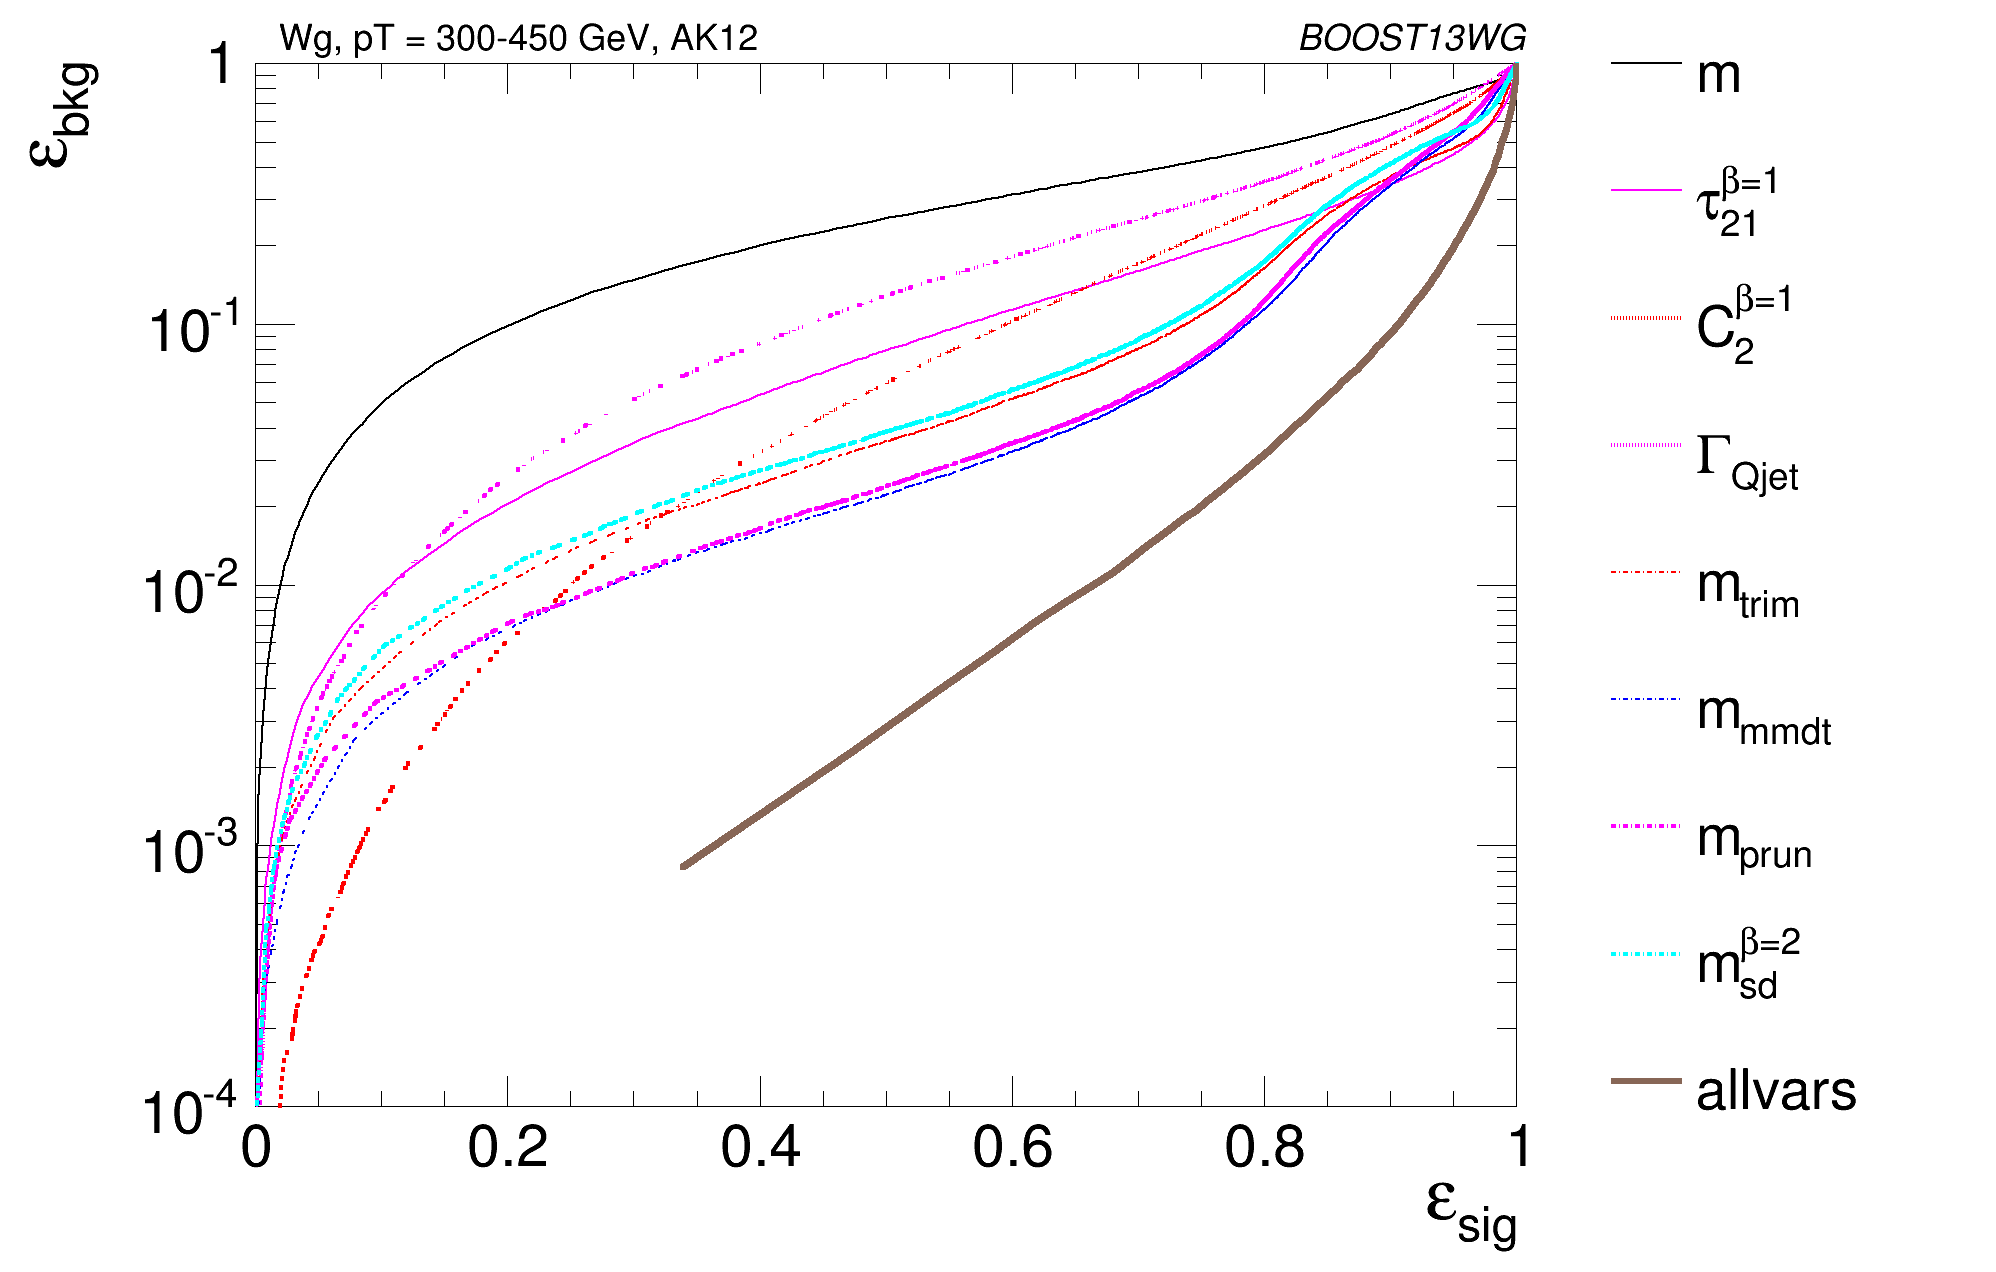
\includegraphics[width=0.48\textwidth]{./Figures/WTagging/pT300/AKtR12/Rocs_1D_single.png}}
\caption{The ROC curve for all single variables considered for $W$
tagging in the \pt 300-400 GeV bin using the anti-\kT R=0.8 algorithm and R=1.2 algorithm.}
\label{fig:pt300_single}
\end{center}
\end{figure*}


\begin{figure*}
\begin{center}
\subfigure[\antikt R=0.8, \pt 500-600 GeV bin]{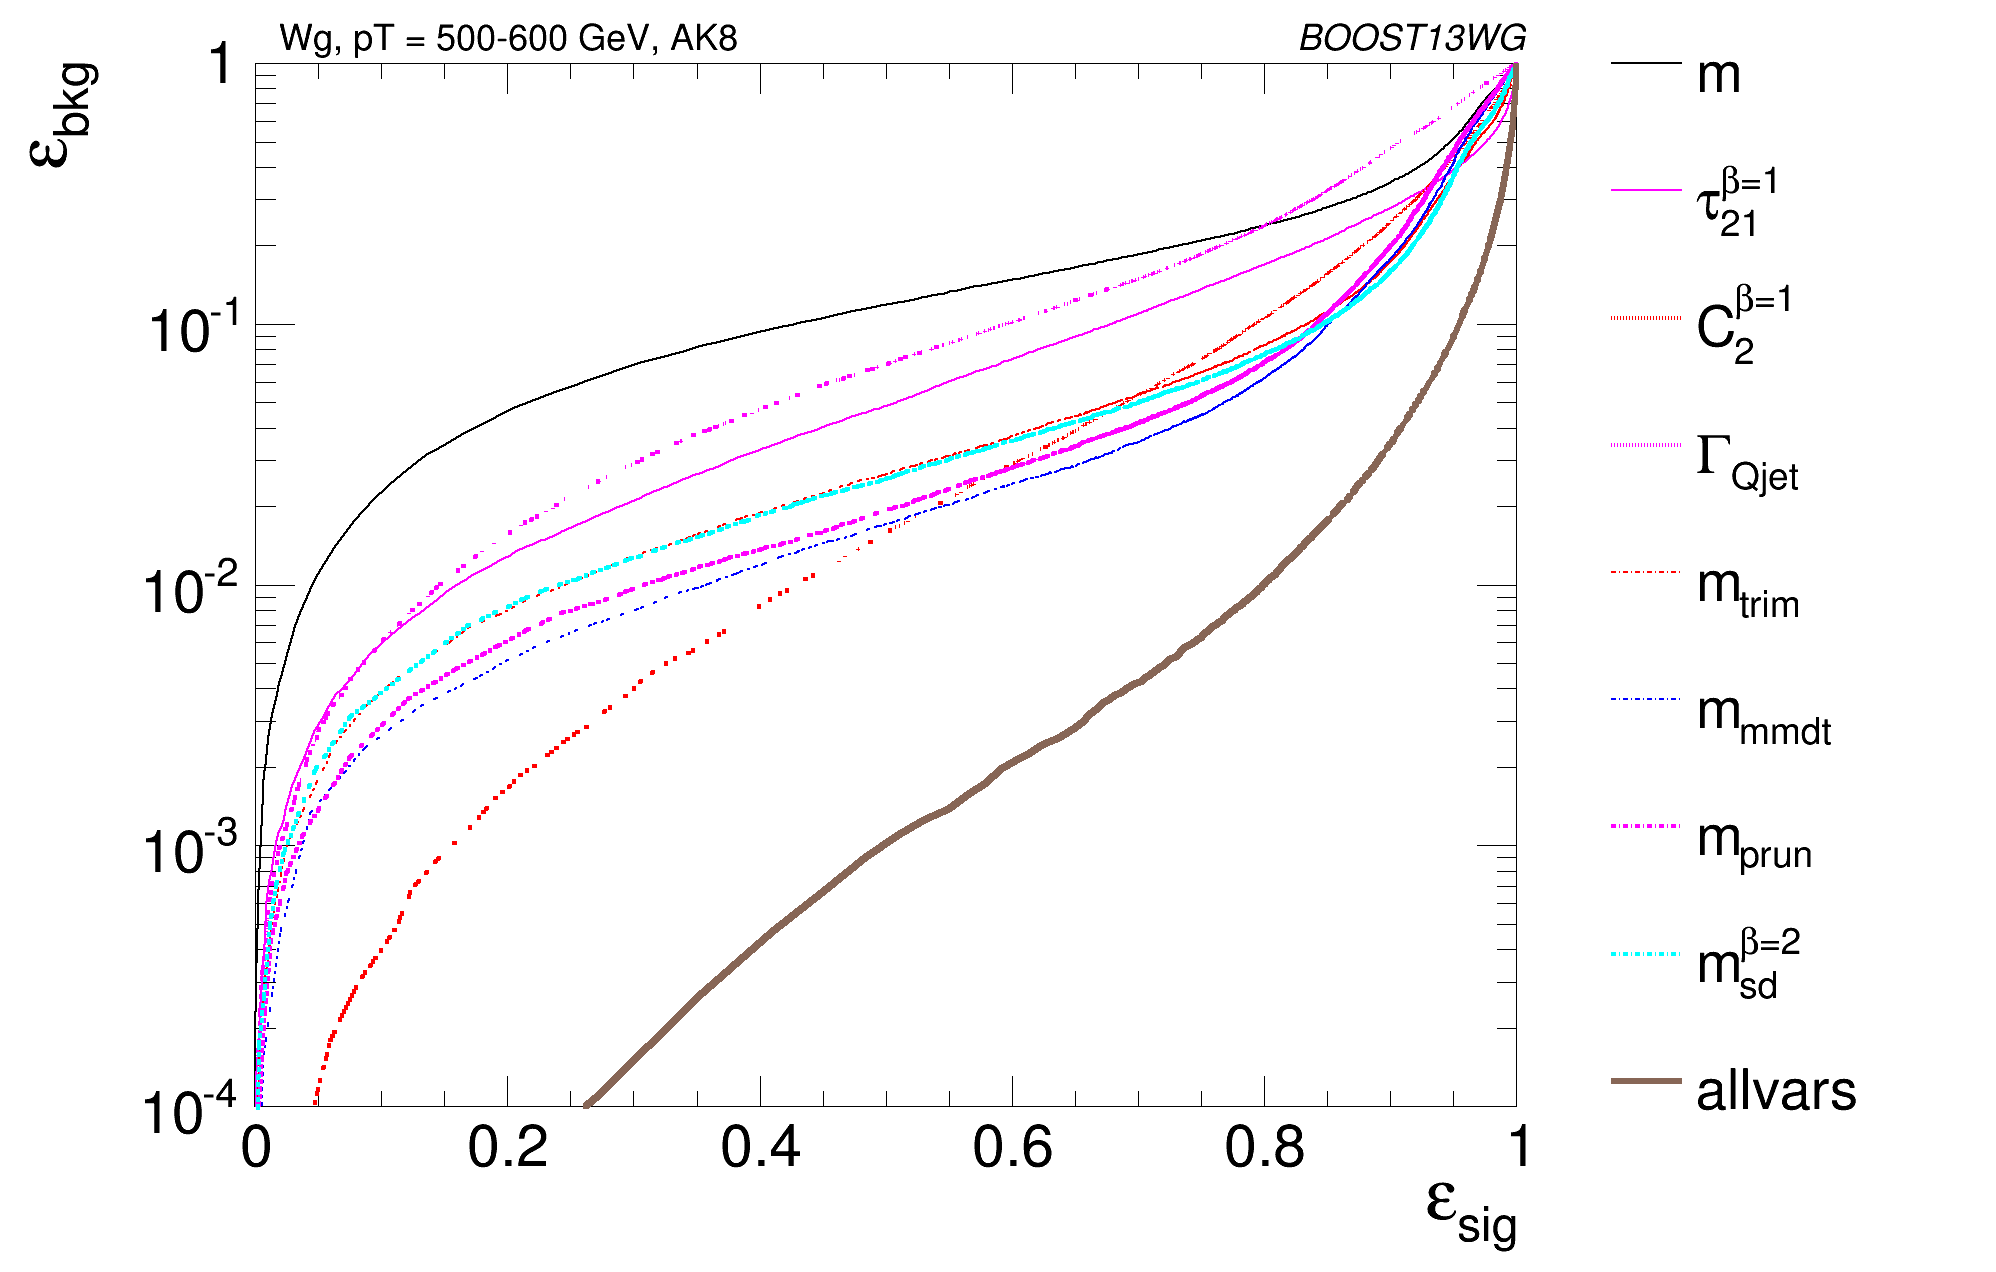
\includegraphics[width=0.48\textwidth]{./Figures/WTagging/pT500/AKtR08/Rocs_1D_single.png}}
\subfigure[\antikt R=1.2, \pt 500-600 GeV bin]{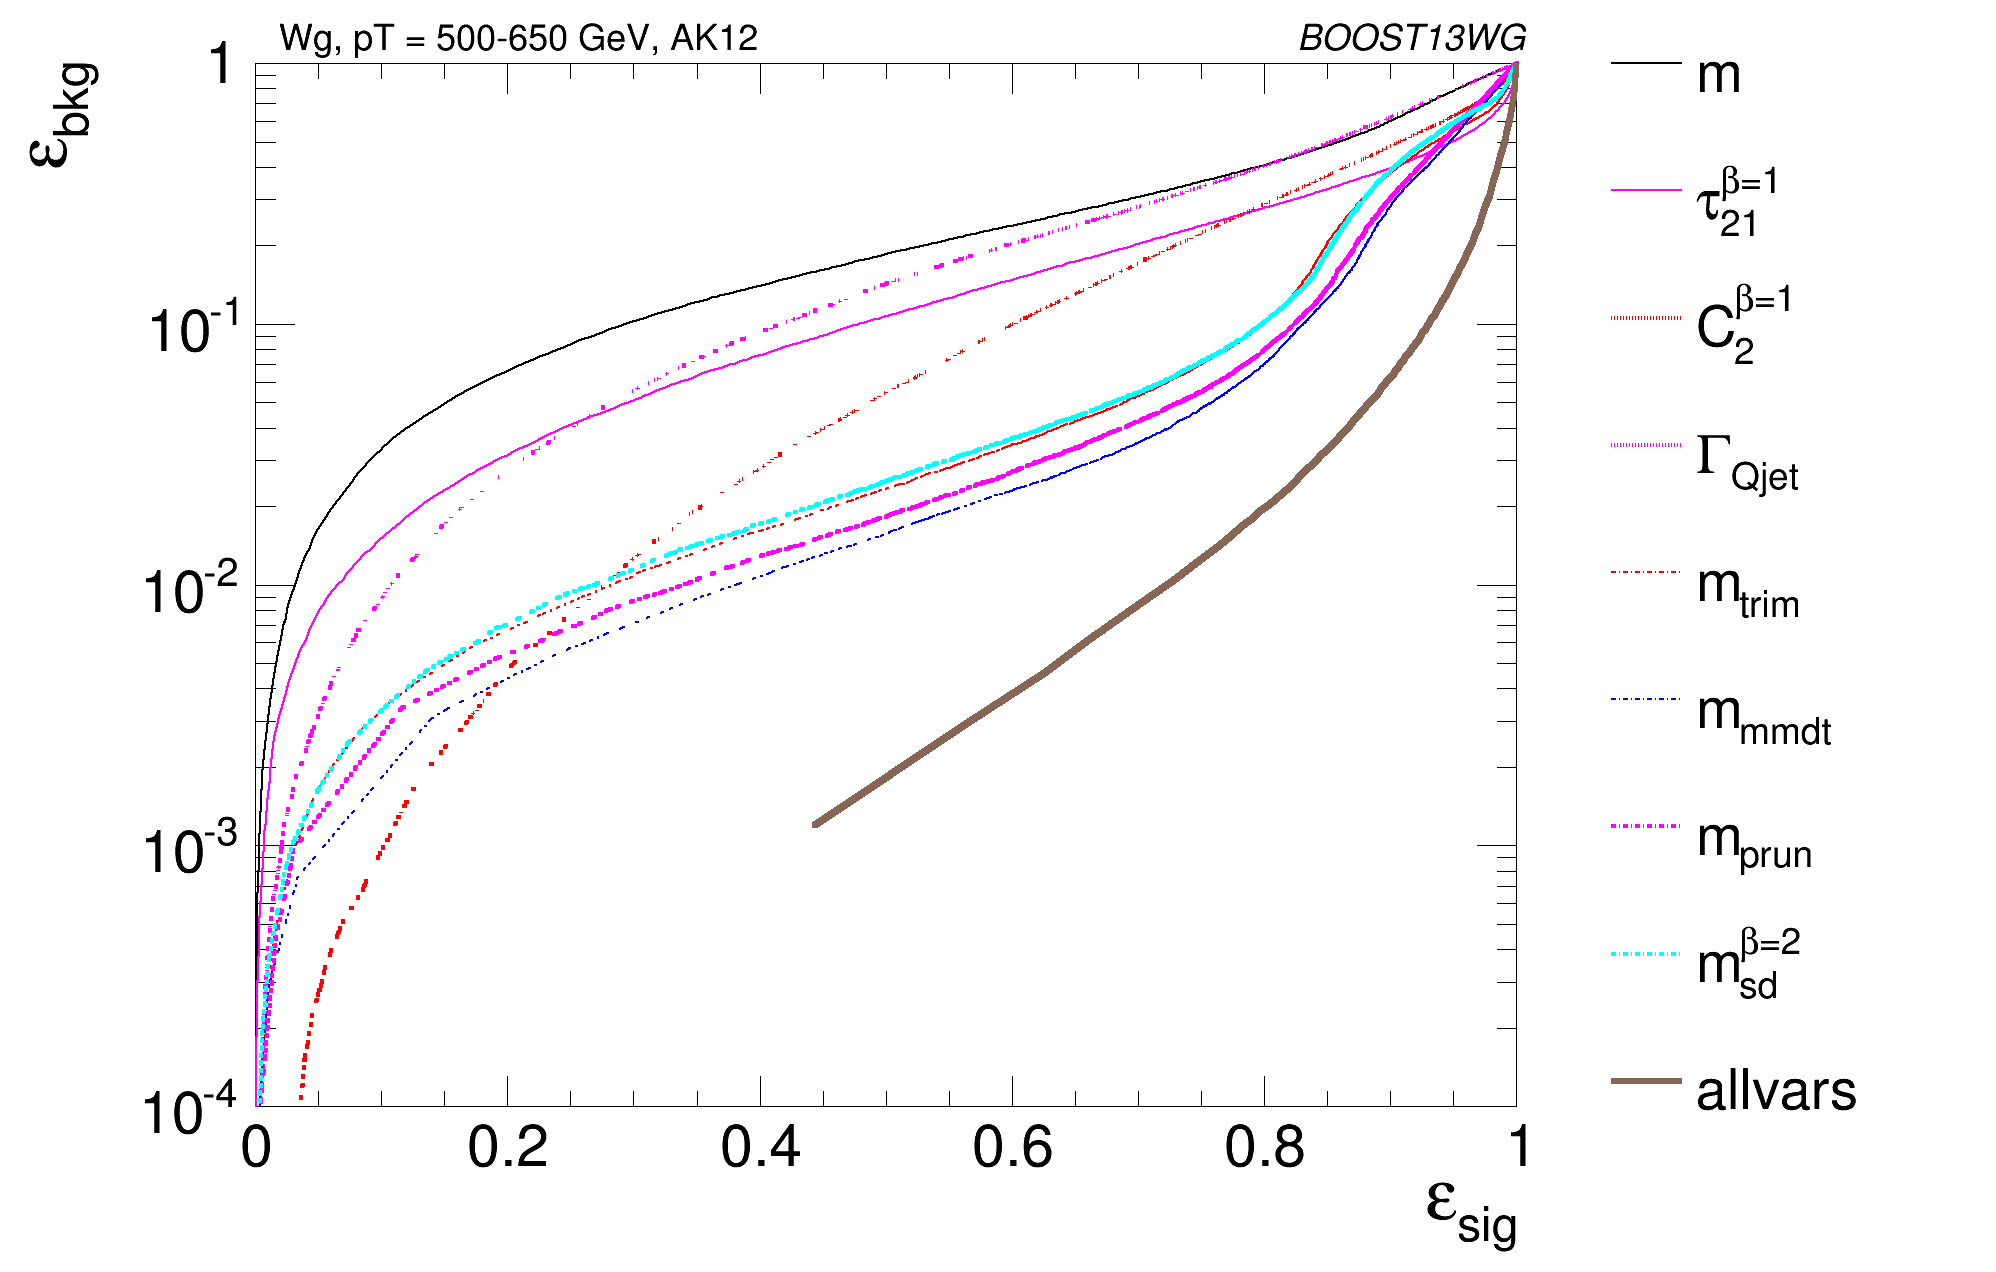
\includegraphics[width=0.48\textwidth]{./Figures/WTagging/pT500/AKtR12/Rocs_1D_single.png}}
\caption{The ROC curve for all single variables considered for $W$
tagging in the \pt 500-600 GeV bin using the anti-\kT R=0.8 algorithm and R=1.2 algorithm.}
\label{fig:pt500_single}
\end{center}
\end{figure*}

\begin{figure*}
\begin{center}
\subfigure[\antikt R=0.4, \pt 1.0-1.1 TeV bin]{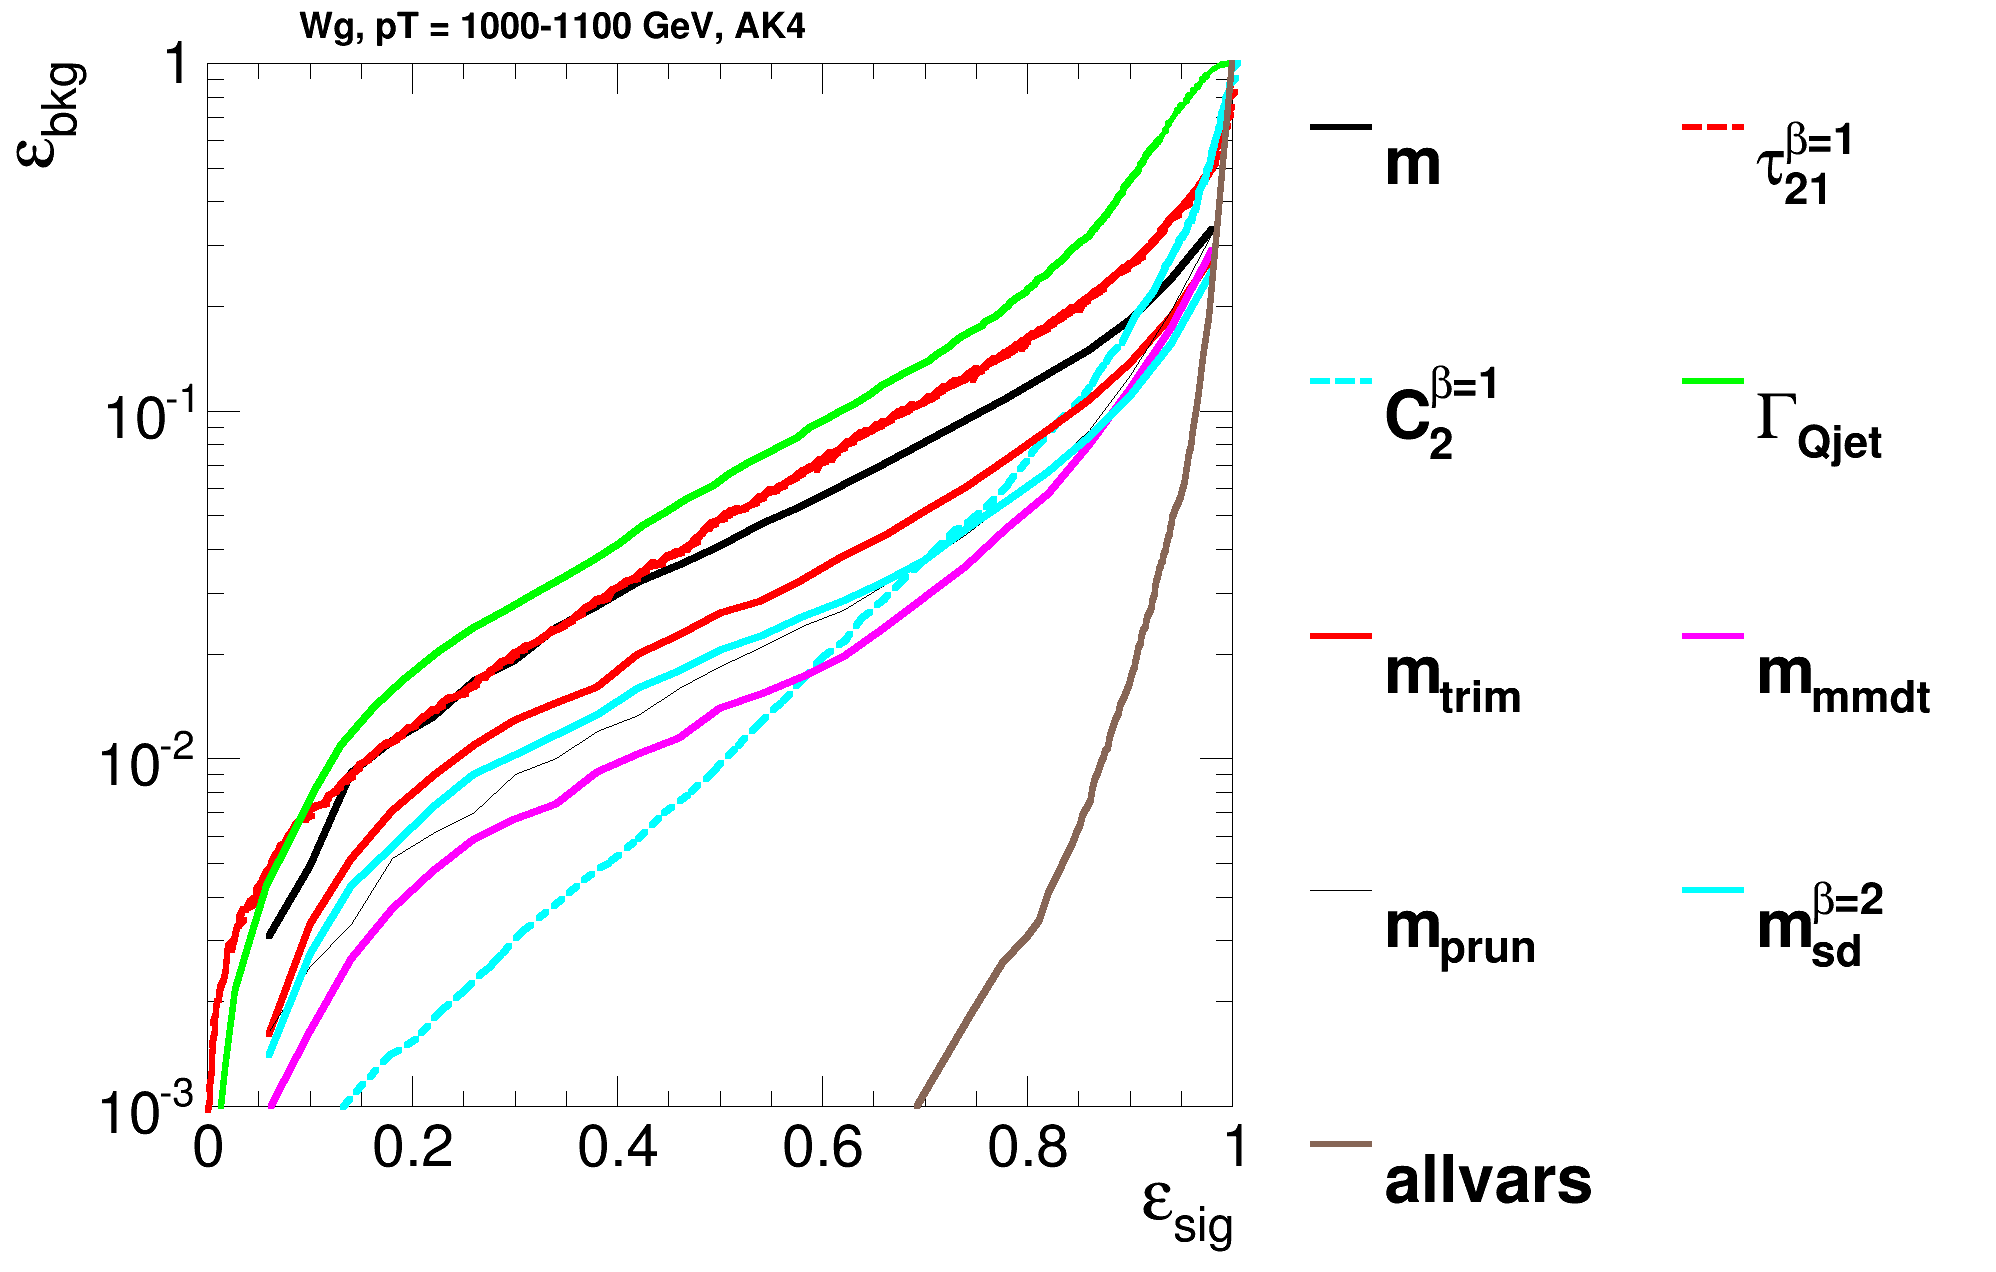
\includegraphics[width=0.48\textwidth]{./Figures/WTagging/pT1000/AKtR04/Rocs_1D_single.png}}
\subfigure[\antikt R=0.8, \pt 1.0-1.1 TeV bin]{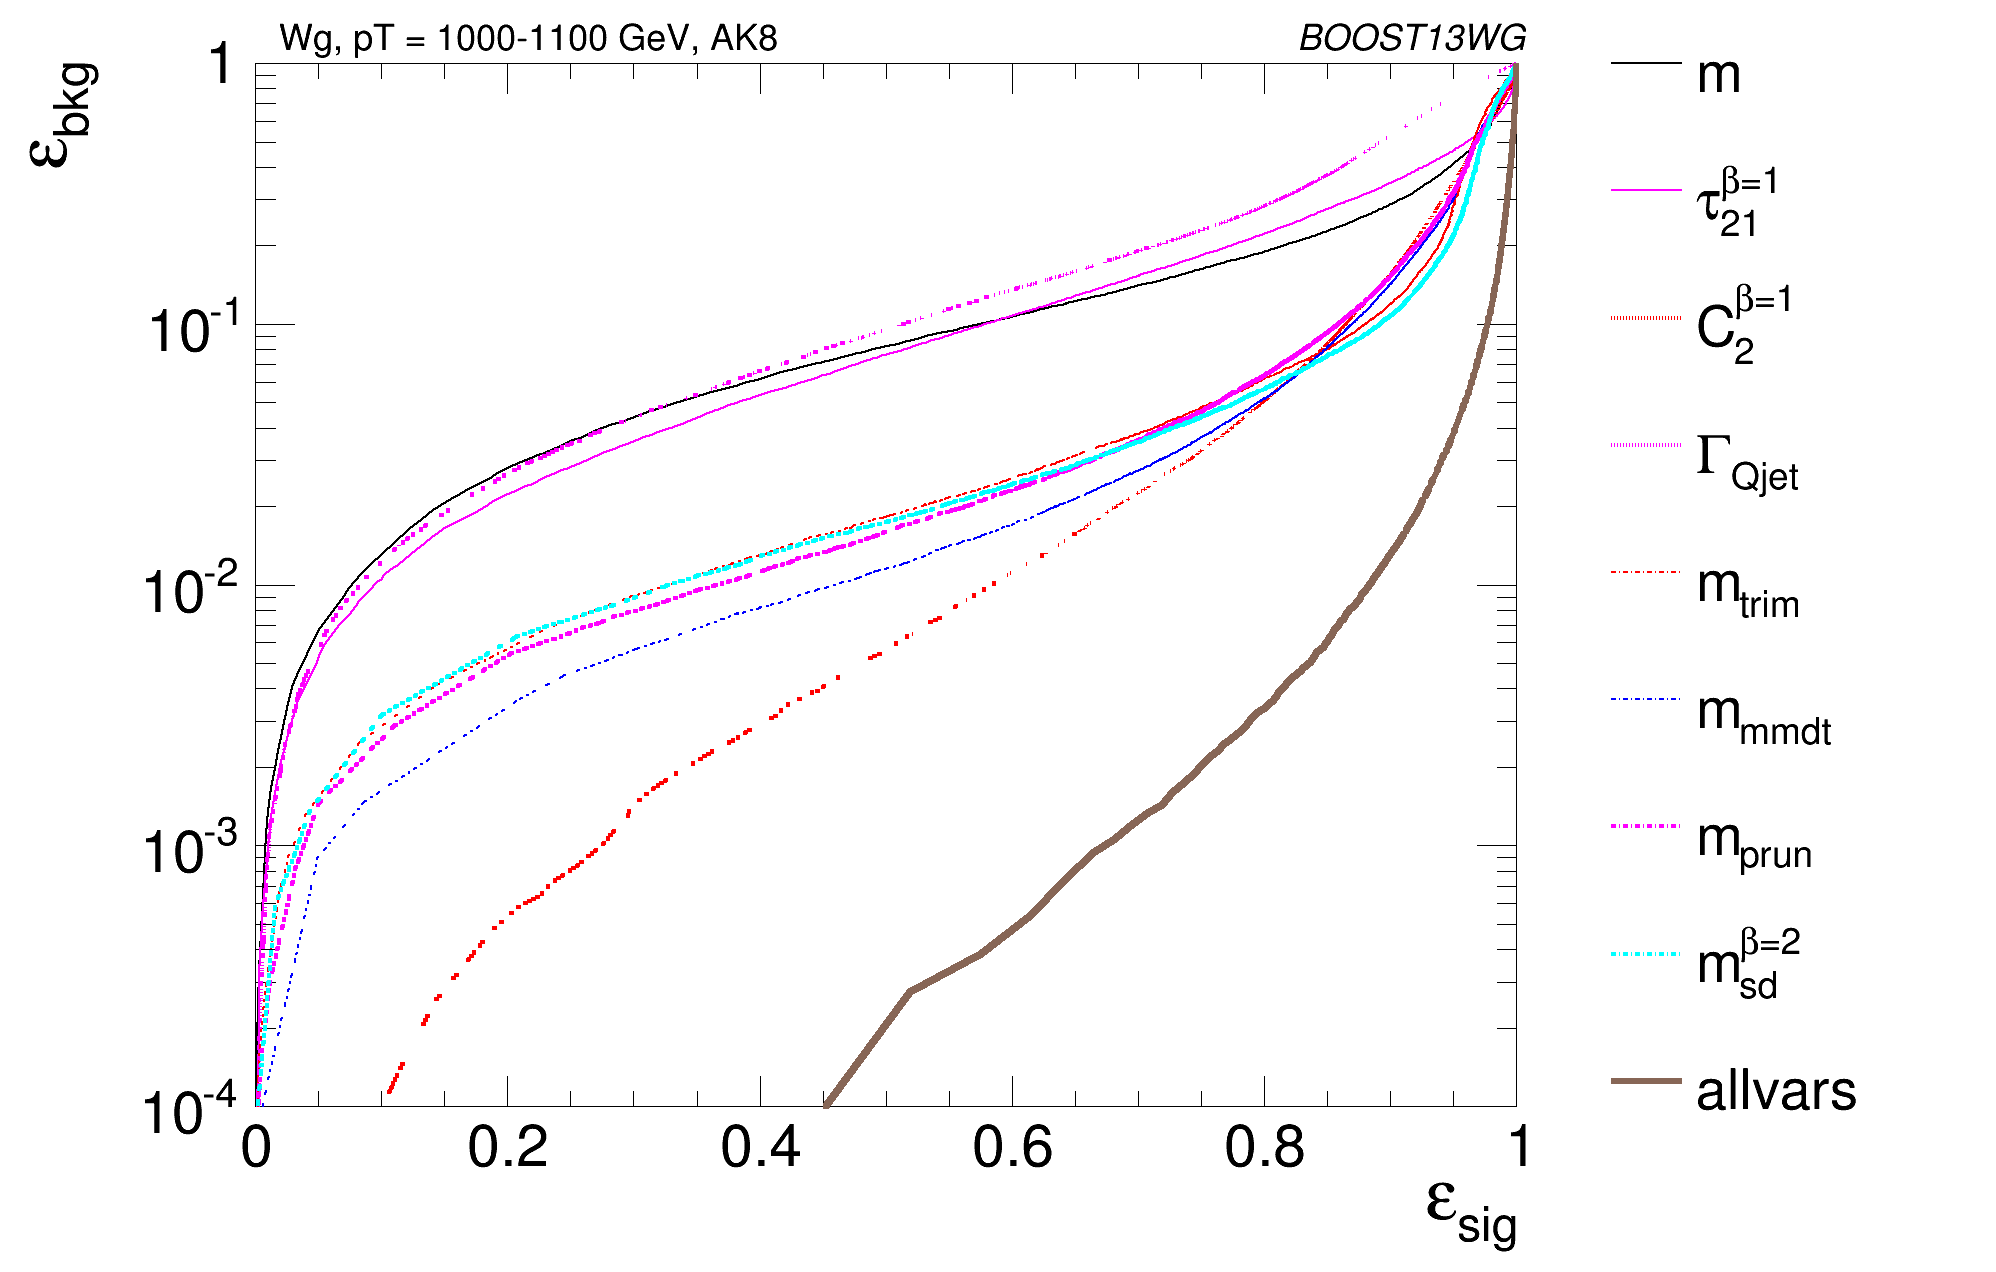
\includegraphics[width=0.48\textwidth]{./Figures/WTagging/pT1000/AKtR08/Rocs_1D_single.png}}\\
\subfigure[\antikt R=1.2, \pt 1.0-1.1 TeV bin]{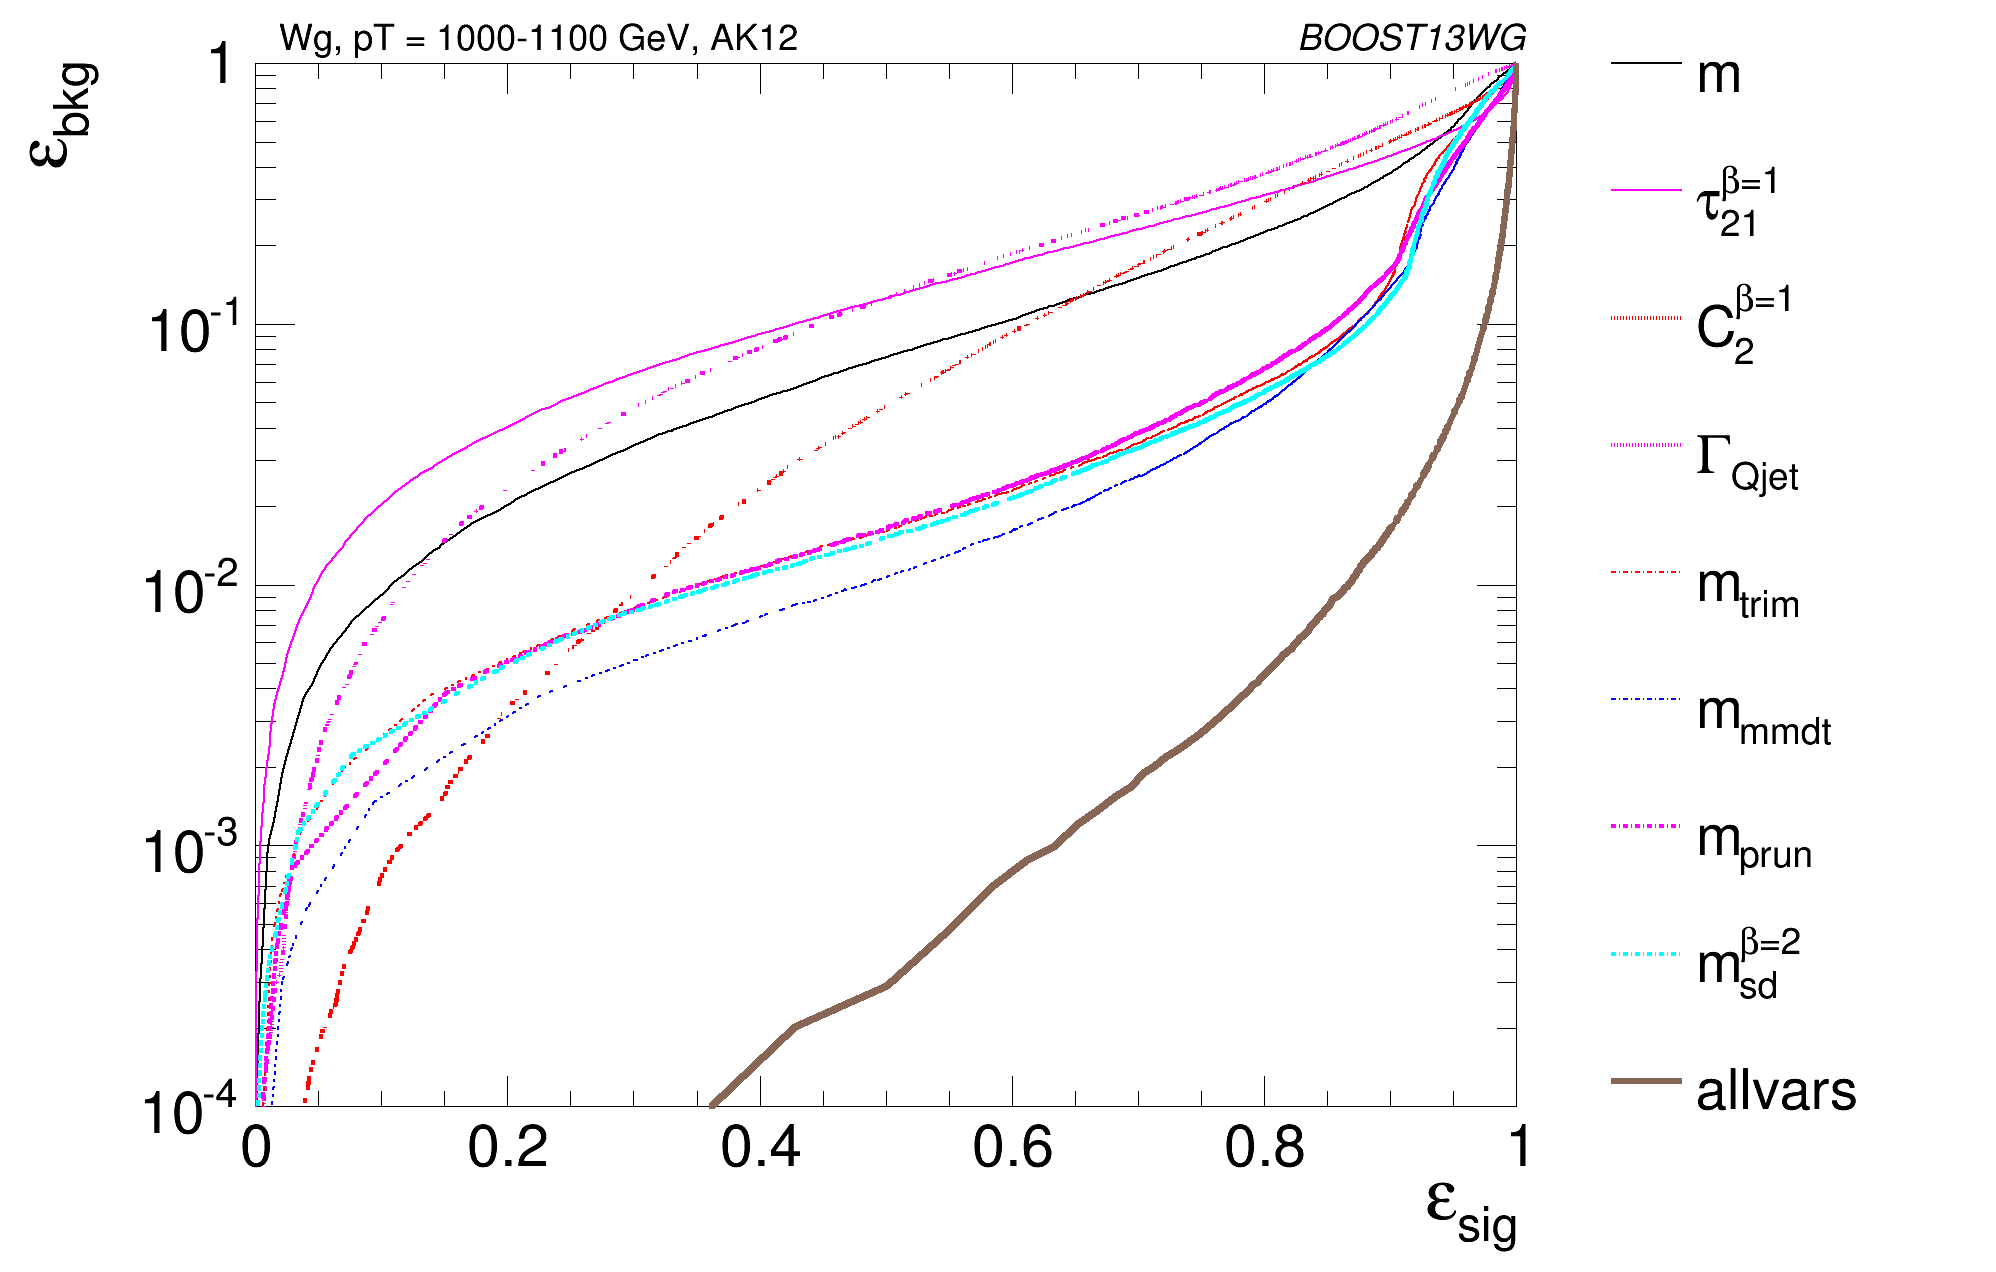
\includegraphics[width=0.48\textwidth]{./Figures/WTagging/pT1000/AKtR12/Rocs_1D_single.png}}
\caption{The ROC curve for all single variables considered for $W$
tagging in the \pt 1.0-1.1 TeV bin using the anti-\kT R=0.4 algorithm,
anti-\kT R=0.8 algorithm and R=1.2 algorithm.}
\label{fig:pt1000_single}
\end{center}
\end{figure*}

%Figure~\ref{fig:pt500_single_AKt_R12} shows the single variable ROC curves in
%the \pT 500 GeV bin for the anti-\kT R=1.2 algorithm, compared to the
%ROC curve for a BDT combination of all the variables. Comparing to
%Figure~\ref{fig:pt500_single_AKt_R08}, one can see that the
%performance of the groomed masses is quite similar. However, the
%performance of the other non-mass substructure variables is markedly
%different, and better in the R=0.8 case.
%
%\begin{figure*}
%\begin{center}
%\includegraphics[width=0.8\textwidth]{./Figures/figs072514/figs071614_Wg_bin500_ak12/Rocs_1D_single.png}
%\caption{The ROC curve for all single variables considered for $W$
%tagging in the \pt 500 GeV bin using the anti-\kT R=1.2 algorithm.}
%\label{fig:pt500_single_AKt_R12}
%\end{center}
%\end{figure*}

Although the ROC curves give all the relevant information, it is hard
to compare performance quantitatively. In
Figures~\ref{fig:pt300_comb2D},~\ref{fig:pt500_comb2D}
and~\ref{fig:pt1000_comb2D} are shown matrices which give the
background rejection for a signal efficiency of 70\% when two
variables (that on the x-axis and that on the y-axis) are combined in
a BDT. These are shown separately for each \pt~bin and jet radius
considered. In the
final column of these plots are shown the background rejection
performance for three-variable BDT combinations of $m_{sd}^{\beta=2} +
C_2^{\beta=1} + X$. These results will be discussed later in Section~\ref{sec:Wtagallvars}. The diagonal of these plots correspond to the background
rejections for a single variable BDT, and can thus be examined to get a
quantitative measure of the individual single variable performance,
and to study how this changes with jet radius and momenta. 

One can see that in general the most performant single variables are
the groomed masses. However, in certain kinematic bins and for certain
jet radii, $C_2^{\beta=1}$ has a background rejection that is
comparable to or better than the groomed masses. 

%By comparing Figures~\ref{fig:pt300_comb2D_08}
%and~\ref{fig:pt300_comb2D_12}, Figures 
By comparing
Figures~\ref{fig:pt300_comb2D_08},~\ref{fig:pt500_comb2D_08}
and~\ref{fig:pt1000_comb2D_08}, we can see how the background
rejection performance evolves as we increase momenta whilst keeping the jet
radius fixed to R=0.8. Similarly, by comparing Figures~\ref{fig:pt300_comb2D_12},~\ref{fig:pt500_comb2D_12}
and~\ref{fig:pt1000_comb2D_12} we can see how performance evolves with
\pt~for R=1.2. For both R=0.8 and R=1.2 the background rejection power of
the groomed masses increases with increasing \pt, with a factor 1.5-2.5 increase in rejection in going from the 300-400 GeV to
1.0-1.1 TeV bins. {\bf ED: Add some of the 1-D plots comparing signal and bkgd
  in the different masses and pT bins here?} However, the $C_2^{\beta=1}$, $\Gamma_{Qjet}$ and
$\tau_{21}^{\beta=1}$ substructure variables behave somewhat
differently. The background rejection power of the $\Gamma_{Qjet}$ and
$\tau_{21}^{\beta=1}$ variables both decrease with increasing \pt, by
up to a factor two in going from the 300-400 GeV to
1.0-1.1 TeV bins. Conversely the rejection power of $C_2^{\beta=1}$
dramatically increases with increasing \pt~for R=0.8, but does not
improve with \pt~for the larger jet radius R=1.2. {\bf ED: Can we
  explain this? Again, should we add some of the 1-D plots?}

By comparing the individual sub-figures of Figures~\ref{fig:pt300_comb2D},~\ref{fig:pt500_comb2D}
and~\ref{fig:pt1000_comb2D} we can see how the background rejection
performance depends on jet radius within the same \pt bin. To within
$\sim$~25\%, the background rejection power of the groomed masses remains
constant with respect to the jet radius. However, we again see rather
different behaviour for the substructure variables. In all \pt bins
considered the most performant substructure variable, $C_2^{\beta=1}$,
performs best for an \antikt distance parameter of R=0.8. The
performance of this variable is dramatically worse for the larger jet
radius of R=1.2 (a factor seven worse background rejection in
the 1.0-1.1 TeV bin), and substantially worse for R=0.4. For the other
jet substructure variables considered, $\Gamma_{Qjet}$ and
$\tau_{21}^{\beta=1}$, their background rejection
power also reduces for larger jet radius, but not to the same extent.
{\bf
  ED: Insert some nice discussion/explanation of why jet substructure
  power generally gets worse as we go to large jet radius, but groomed
mass performance does not. Probably need the 1-D figures for this.}

%The best performant individual variables for a reasonable signal
%efficiency are the groomed masses, which all have a similar
%level of performance that is superior to that of any of the
%substructure variables considered. 
%
%Because we
%have not attempted to optimise the grooming parameter settings of
%each grooming algorithm, we do not want to place too much emphasis
%here on the relative performance of the groomed masses, but instead
%look at the trends veresus \pt and R. One
%can see clearly that the background rejection power of the groomed mass
%variables increases as the \pt is increased. Within a \pt
%bin, one can also see that the groomed mass performance is rather invariant to
%changes in the jet radius. In contrast, the substructure variable
%performance varies considerably as the jet radius is changed. In
%general, the background rejection power of individual jet substructure
%variables gets worse as the jet radius is increased. The only
%exception to this is in the highest \pt~bin, where the background
%rejection power of $C_2^{\beta=1}$ improves when going from jet radius
%R=0.4 to R=0.8, but then gets worse again as we go to R=1.2. {\it
%  Insert some nice discussion/explanation of why jet substructure
%  power generally gets worse as we go to large jet radius, but groomed
%mass performance does not}

\begin{figure*}
\begin{center}
\subfigure[\antikt R=0.8, \pt 300-400 GeV bin]{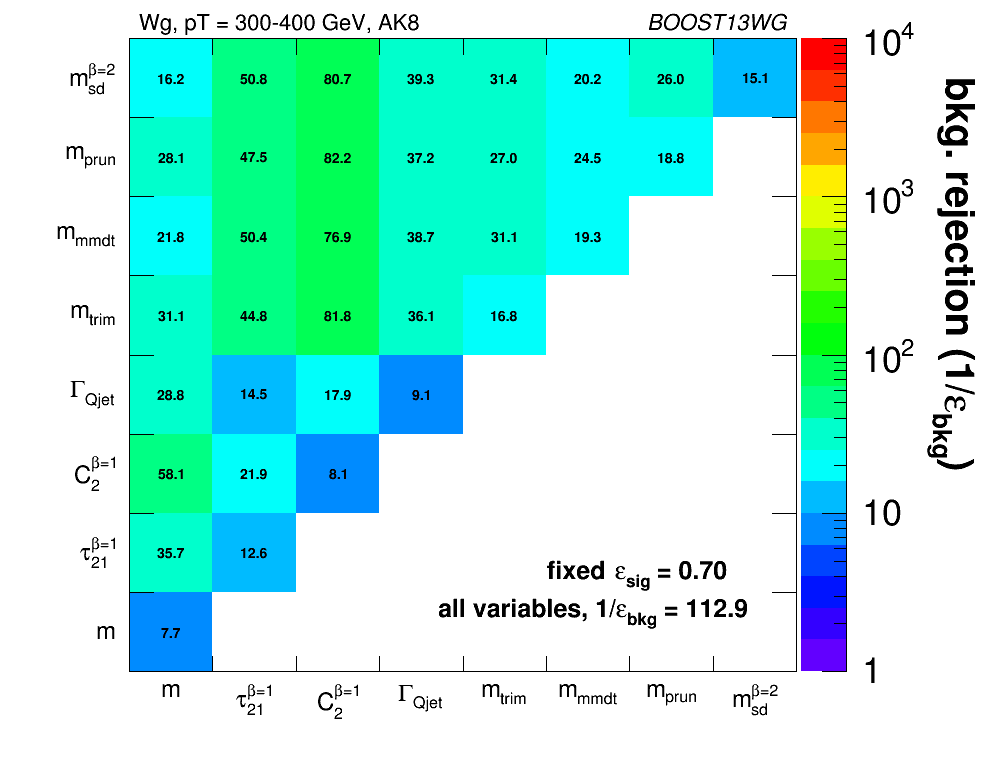
\includegraphics[width=0.48\textwidth]{./Figures/WTagging/pT300/AKtR08/effBkg2D.png}\label{fig:pt300_comb2D_08}}
\subfigure[\antikt R=1.2, \pt 300-400 GeV bin]{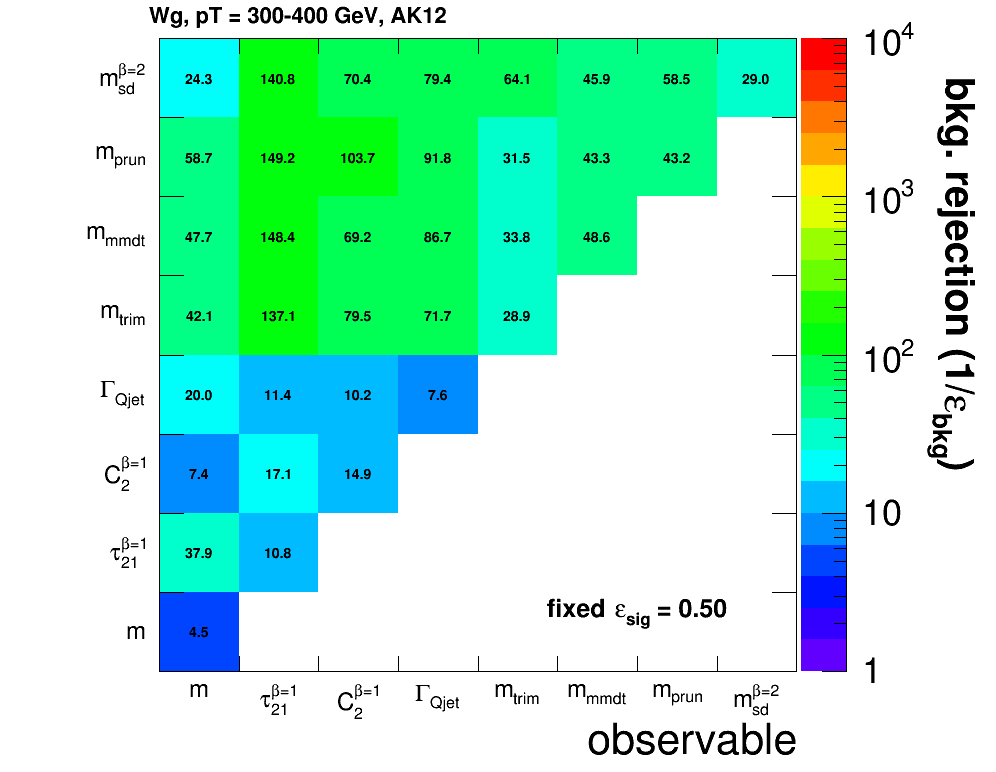
\includegraphics[width=0.48\textwidth]{./Figures/WTagging/pT300/AKtR12/effBkg2D.png}\label{fig:pt300_comb2D_12}}
\caption{
The background rejection
for a fixed signal efficiency (70\%) of each BDT combination of
each pair of variables considered, in the \pt 300-400 GeV bin using the anti-\kT R=0.8
algorithm and R=1.2 algorithm. Also shown is the background rejection
for a BDT combination of all of the variables considered.
}
\label{fig:pt300_comb2D}
\end{center}
\end{figure*}


\begin{figure*}
\begin{center}
\subfigure[\antikt R=0.8, \pt 500-600 GeV bin]{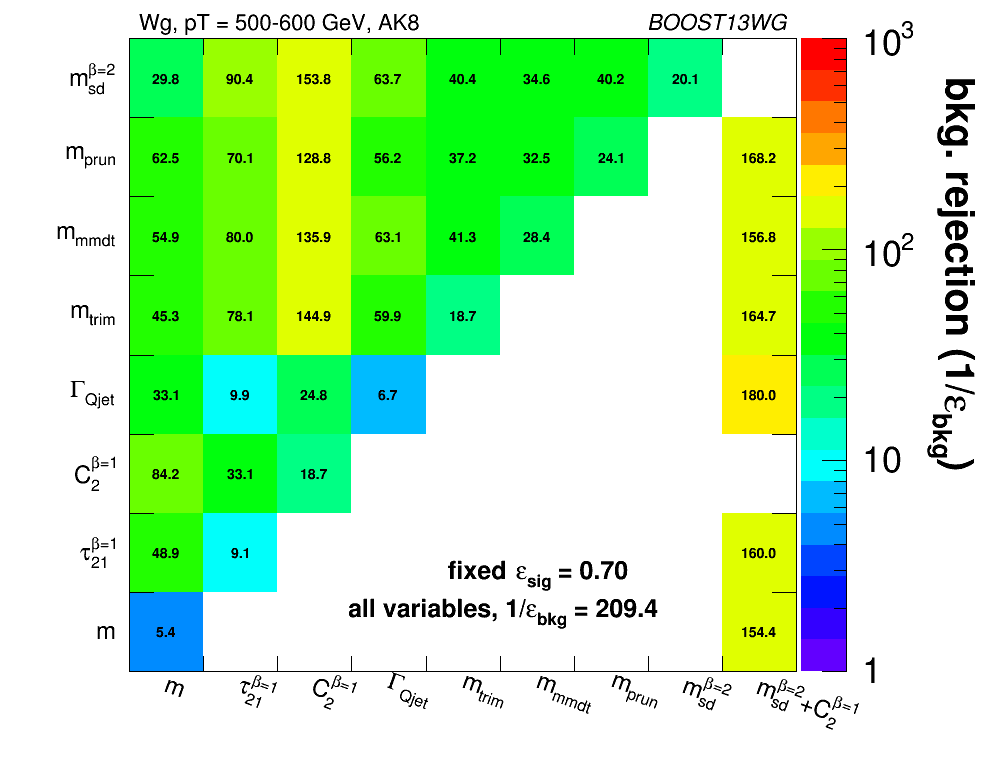
\includegraphics[width=0.48\textwidth]{./Figures/WTagging/pT500/AKtR08/effBkg2D.png}\label{fig:pt500_comb2D_08}}
\subfigure[\antikt R=1.2, \pt 500-600 GeV bin]{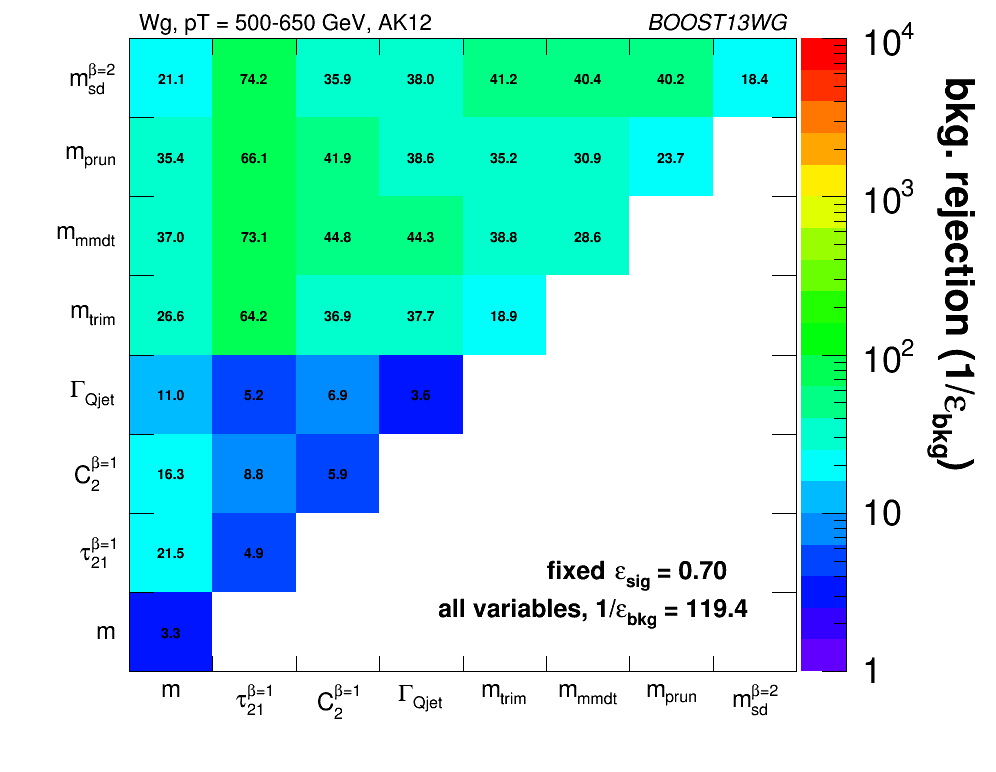
\includegraphics[width=0.48\textwidth]{./Figures/WTagging/pT500/AKtR12/effBkg2D.png}\label{fig:pt500_comb2D_12}}
\caption{The background rejection
for a fixed signal efficiency (70\%) of each BDT combination of
each pair of variables considered, in the \pt 500-600 GeV bin using the anti-\kT R=0.8
algorithm and R=1.2 algorithm. Also shown is the background rejection
for a BDT combination of all of the variables considered.}
\label{fig:pt500_comb2D}
\end{center}
\end{figure*}

\begin{figure*}
\begin{center}
\subfigure[\antikt R=0.4, \pt 1.0-1.1 TeV bin]{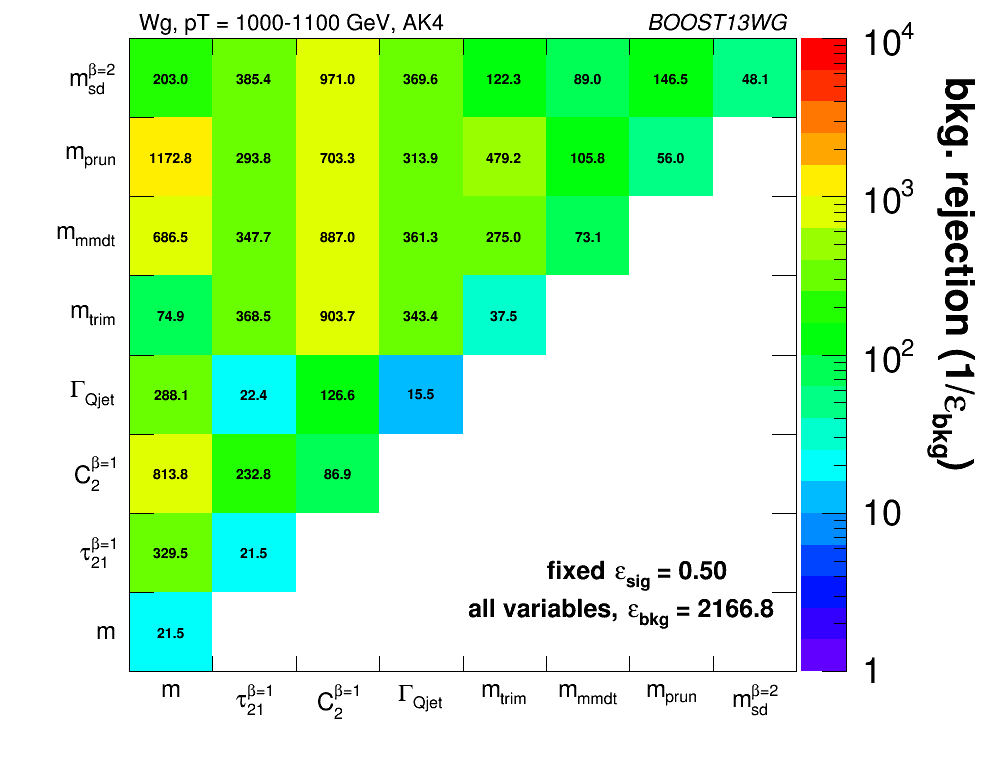
\includegraphics[width=0.48\textwidth]{./Figures/WTagging/pT1000/AKtR04/effBkg2D.png}\label{fig:pt1000_comb2D_04}}
\subfigure[\antikt R=0.8, \pt 1.0-1.1 TeV bin]{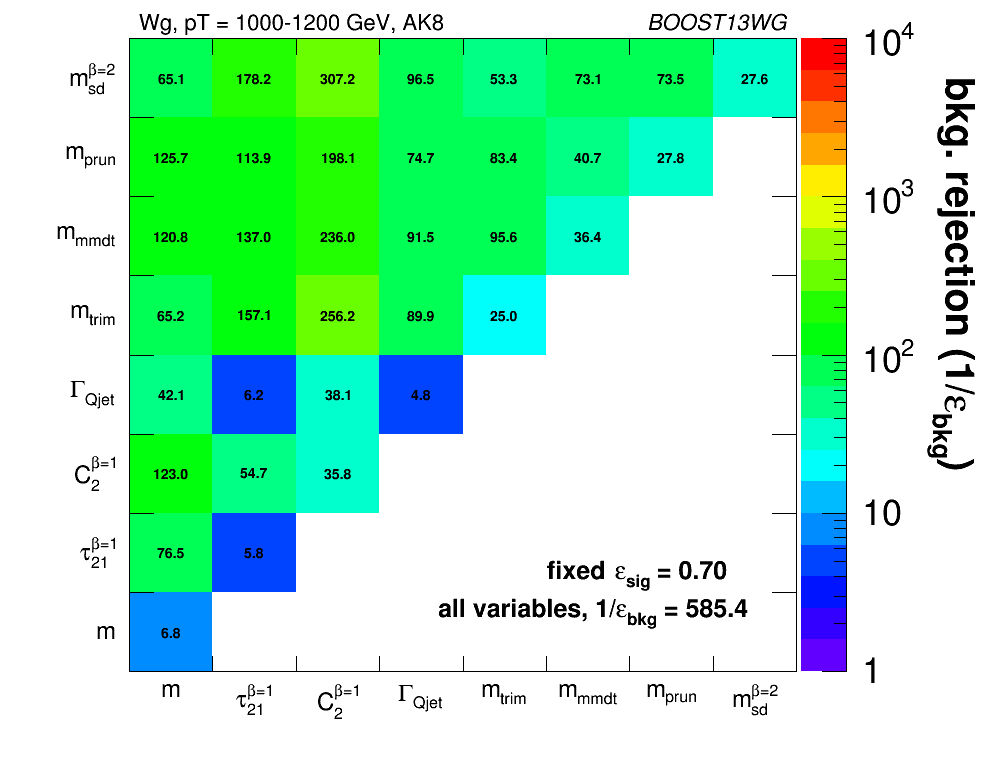
\includegraphics[width=0.48\textwidth]{./Figures/WTagging/pT1000/AKtR08/effBkg2D.png}\label{fig:pt1000_comb2D_08}}\\
\subfigure[\antikt R=1.2, \pt 1.0-1.1 TeV bin]{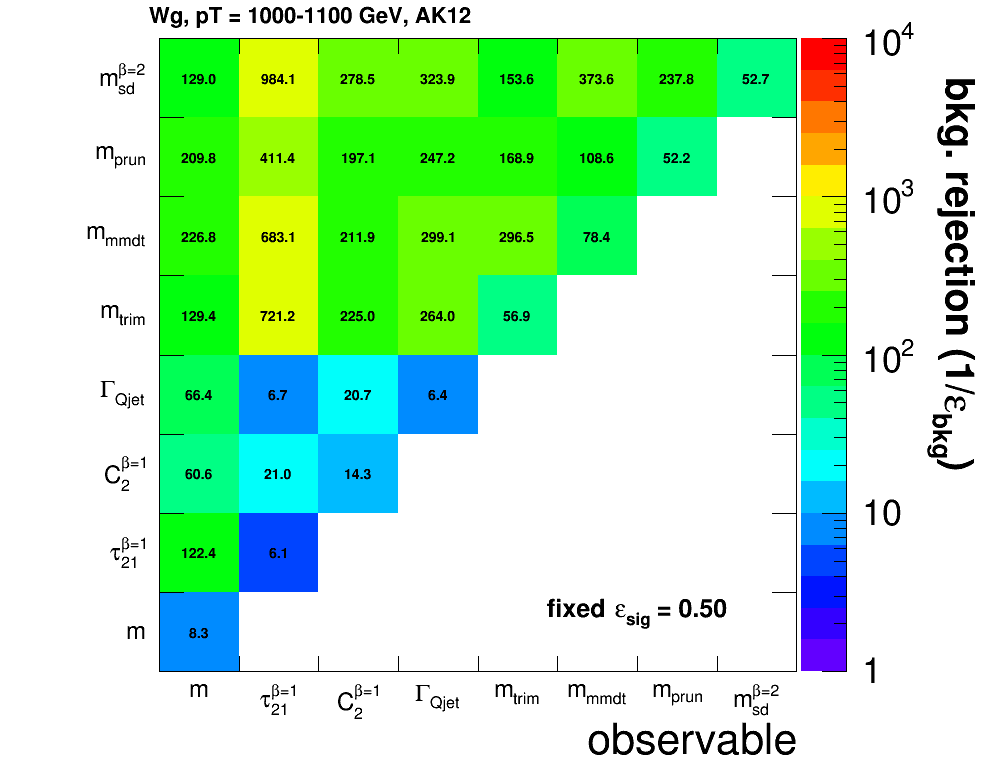
\includegraphics[width=0.48\textwidth]{./Figures/WTagging/pT1000/AKtR12/effBkg2D.png}\label{fig:pt1000_comb2D_12}}
\caption{The background rejection
for a fixed signal efficiency (70\%) of each BDT combination of
each pair of variables considered, in the \pt 1.0-1.1 TeV bin using
the anti-\kT R=0.4, R=0.8 and R=1.2 algorithm. Also shown is the background rejection
for a BDT combination of all of the variables considered.}
\label{fig:pt1000_comb2D}
\end{center}
\end{figure*}


\subsection{Combined Performance}

The off-diagonal entries in Figures~\ref{fig:pt300_comb2D},~\ref{fig:pt500_comb2D}
and~\ref{fig:pt1000_comb2D} can be used to compare the performance
of different BDT two-variable combinations, and see how this varies as
a function of \pt and R. By comparing the background rejection
achieved for the two-variable combinations to the background rejection
of the ``all variables'' BDT, one can understand how much more
discrimination is possible by adding further variables to the
two-variable BDTs.

One can see that in general the most powerful two-variable
combinations involve a groomed mass and a non-mass substructure
variable ($C_2^{\beta=1}$, $\Gamma_{Qjet}$ or
$\tau_{21}^{\beta=1}$). Two-variable combinations of the substructure
variables are not powerful in comparison.  Which particular mass +
substructure variable combination is the most
powerful depends strongly on the \pt and R of the jet, as discussed
in the sections that follow. 

%The background rejection of
%the most powerful mass + substructure combination comes very close to
%that achieved in the ``all variables'' case, indicating that there is
%little to be gained by making a BDT that is more complex, and that
%there is little more complementary information available, at least in
%terms of that which is offered by the variables considered here.

There is also modest improvement in
the background rejection when different groomed masses are combined,
compared to the single variable groomed mass performance, indicating that there is complementary information between the
different groomed masses. In addition, there is an improvement in the
background rejection when the groomed masses are combined with the
ungroomed mass, indicating that grooming removes some useful
discriminatory information from the jet. These observations are
explored further in the section below.

Generally one can see that the R=0.8 jets offer the best two-variable
combined performance in all \pt~bins explored here. This is despite
the fact that in the highest 1.0-1.1 GeV \pt~bin the average
separation of the quarks from the W decay is much smaller than 0.8,
and well within 0.4. This conclusion could of course be susceptible to
pile-up, which is not considered in this study.

%\subsubsection{Dependence on \pt and R}
\subsubsection{Mass + Substructure Performance}
%maybe change title to "Mass + Substructure Performance"
%then can have a final section titled "All Variables Performance"

As already noted, the largest background rejection at 70\% signal
efficiency are in general achieved using those two variable BDT combinations
which involve a groomed mass and a non-mass substructure variable. For
both R=0.8 and R=1.2 jets, the rejection power of these two variable
combinations increases substantially with increasing \pt, at least
within the \pt~range considered here.

For a jet radius of R=0.8, across the full \pt~range considered, the
groomed mass + substructure variable combinations with the
largest background rejection are those which
involve $C_2^{\beta=1}$. For example, in combination with
$m_{sd}^{\beta=2}$, this produces a five-, eight- and fifteen-fold
increase in background rejection compared to using the groomed mass
alone. In Figure~\ref{fig:2d_c2b1_AKt_R08} the low degree of
correlation between $m_{sd}^{\beta=2}$ versus $C_2^{\beta=1}$ that
leads to these large improvements in background rejection can be
seen. One can also see that what little correlation exists is rather
non-linear in nature, changing from a negative to a positive
correlation as a function of the groomed mass, something which helps
to improve the background rejection in the region of the W mass peak.

\begin{figure*}
\begin{center}
\subfigure[\pt 300-400 GeV]{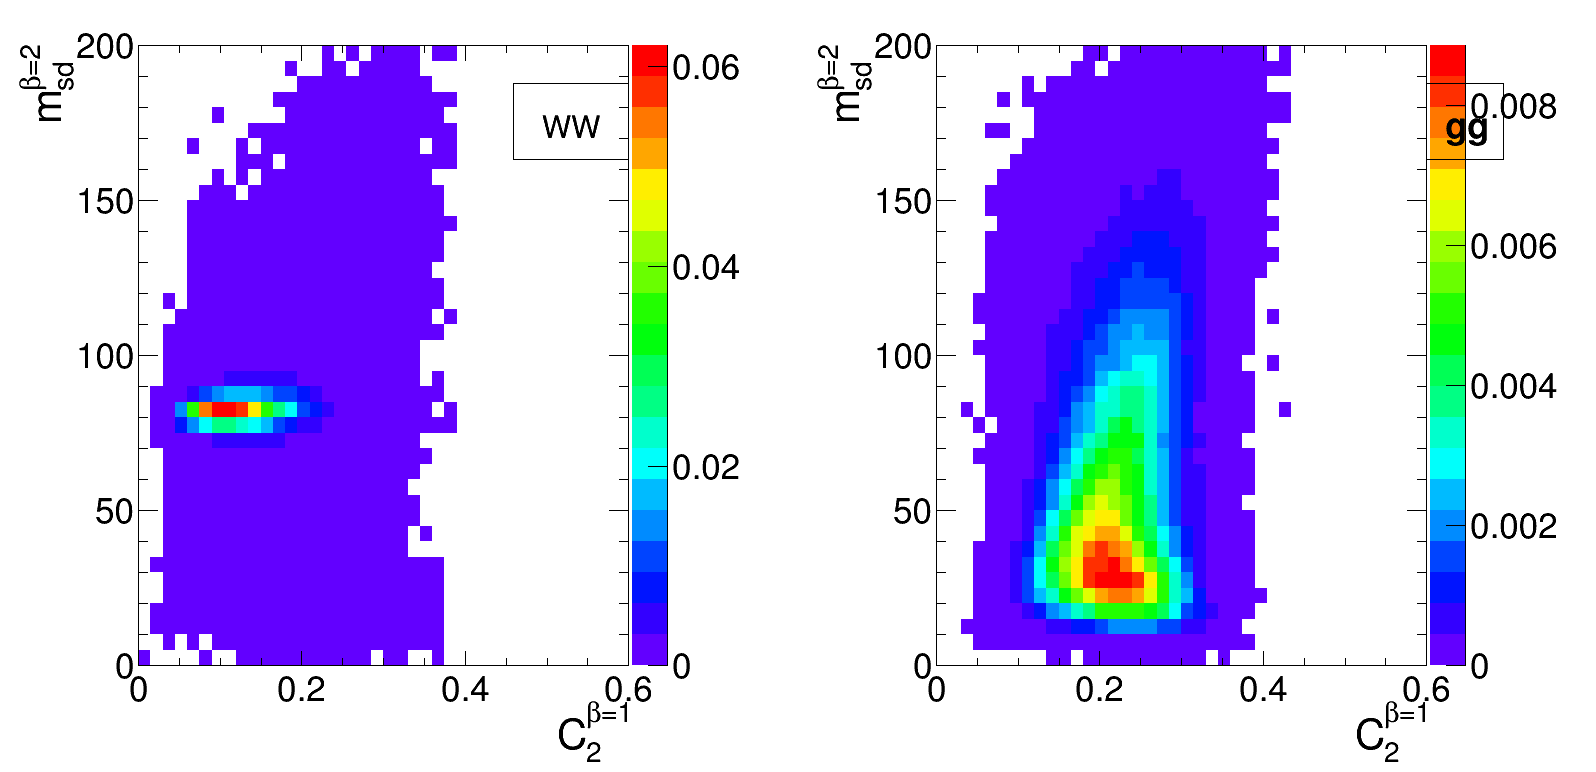
\includegraphics[width=0.78\textwidth]{./Figures/WTagging/pT300/AKtR08/h2d_jc2_b1_j_mass_sdb2_WW_onSame.png}\label{fig:pt300_2d_c2b1_AKt_R08}}
\subfigure[\pt 500-600 GeV]{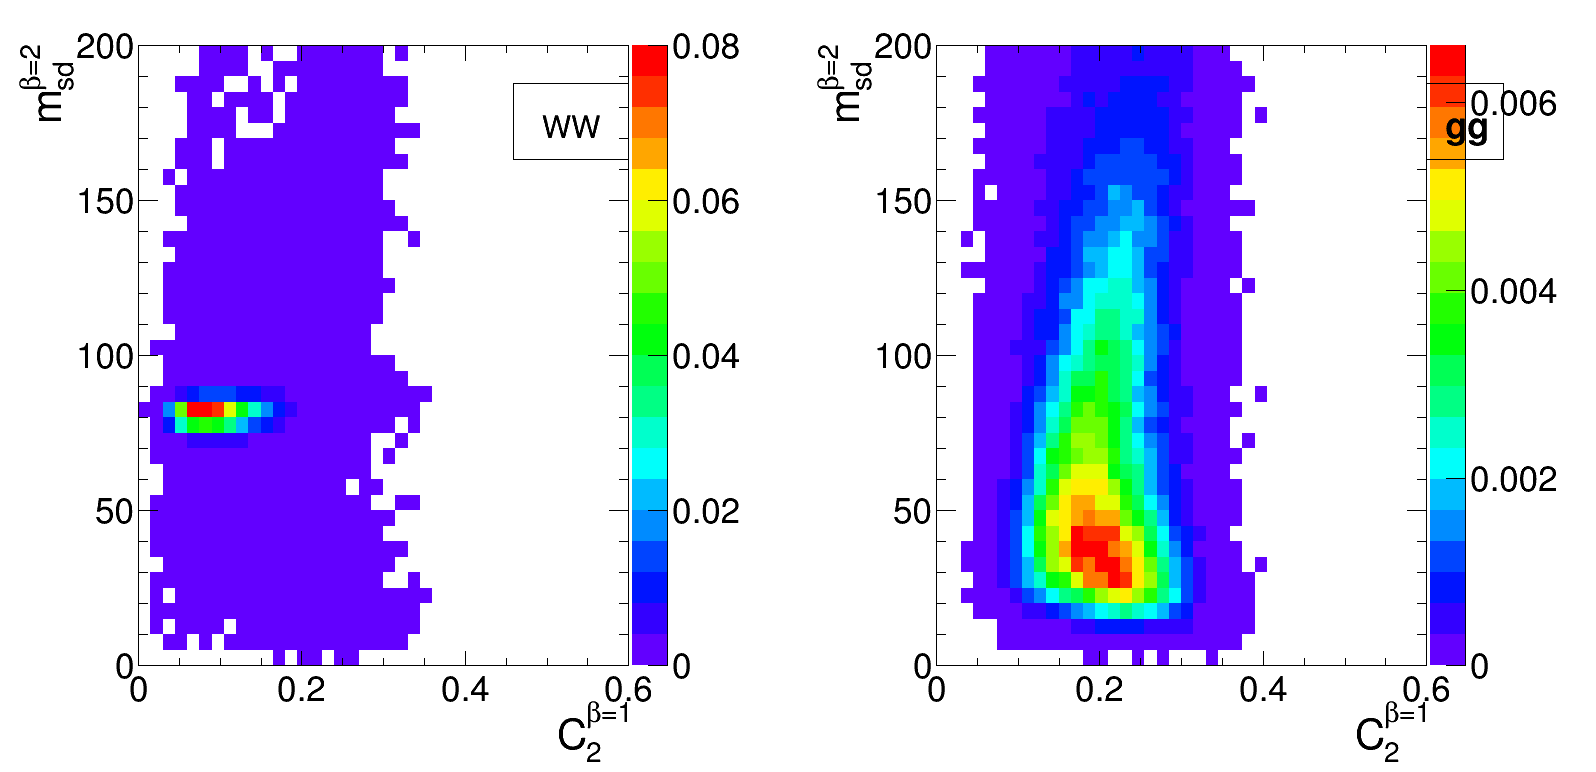
\includegraphics[width=0.78\textwidth]{./Figures/WTagging/pT500/AKtR08/h2d_jc2_b1_j_mass_sdb2_WW_onSame.png}\label{fig:pt500_2d_c2b1_AKt_R08}}
\subfigure[\pt 1.0-1.1 TeV]{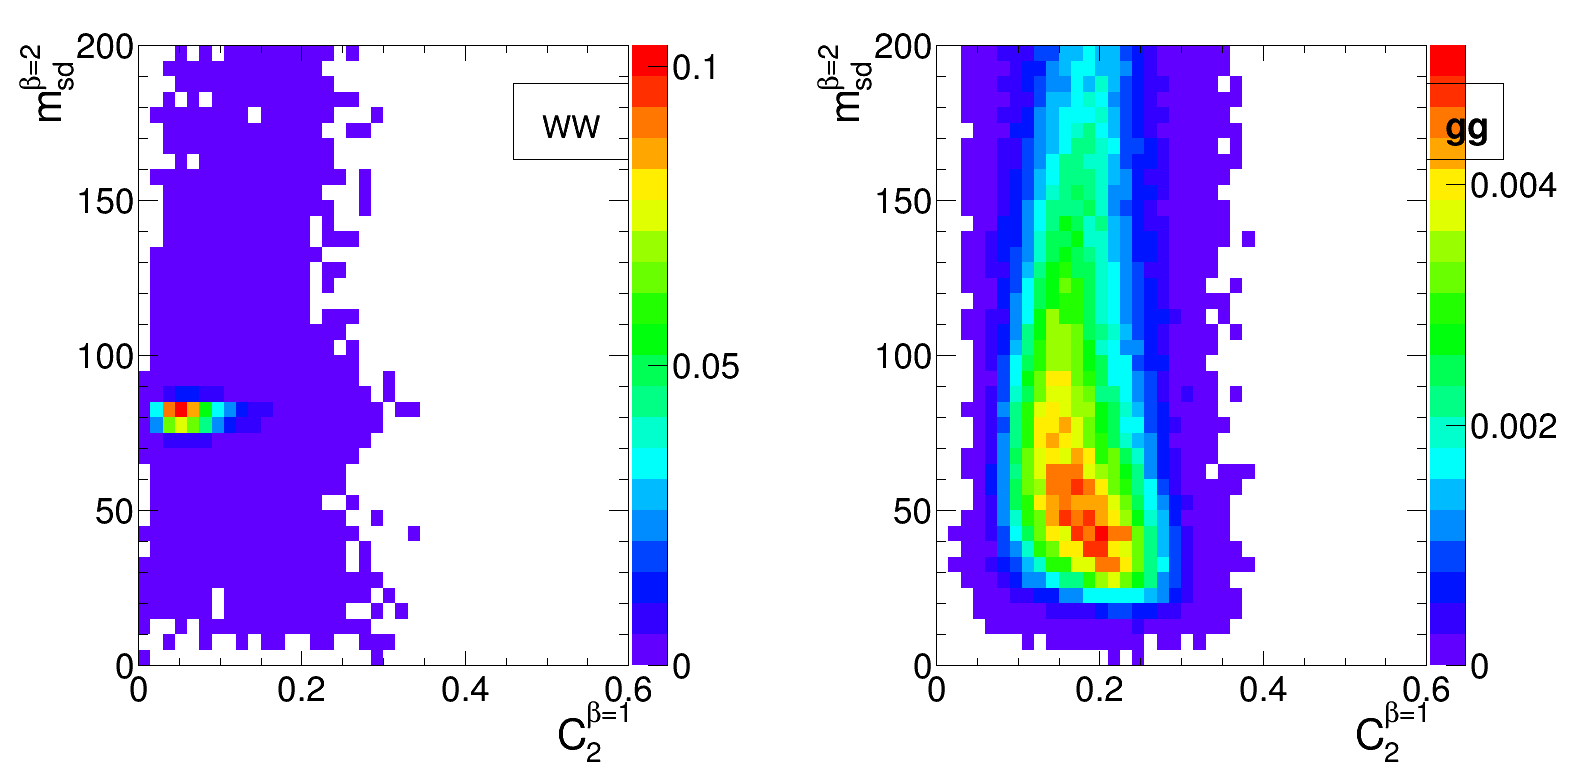
\includegraphics[width=0.78\textwidth]{./Figures/WTagging/pT1000/AKtR08/h2d_jc2_b1_j_mass_sdb2_WW_onSame.png}\label{fig:pt1000_2d_c2b1_AKt_R08}}
\caption{2-D plots showing $m_{sd}^{\beta=2}$ versus $C_2^{\beta=1}$
  for R=0.8 jets in the various \pt~bins considered.}
\label{fig:2d_c2b1_AKt_R08}
\end{center}
\end{figure*}


However, when we switch to a jet radius of R=1.2 the picture for
$C_2^{\beta=1}$ combinations changes dramatically. These become
significantly less powerful, and the most powerful variable in groomed
mass combinations becomes $\tau_{21}^{\beta=1}$ for all jet
\pt~considered. Figure~\ref{fig:2d_c2b1_pt1000} shows the correlation between
$m_{sd}^{\beta=2}$ and $C_2^{\beta=1}$ in the \pt 1.0 - 1.2 TeV bin for
the various jet radii considered. Figure~\ref{fig:2d_tau21_pt1000} is
the equivalent set of distributions for $m_{sd}^{\beta=2}$ and
$\tau_{21}^{\beta=1}$. One can see from
Figure~\ref{fig:2d_c2b1_pt1000} that, due to the sensitivity of the
observable to to soft, wide-angle radiation, as the jet radius increases
$C_2^{\beta=1}$ increases and becomes more and more smeared out for both signal and
background, leading to worse discrimination power. This does not
happen to the same extent for $\tau_{21}^{\beta=1}$. We can see from Figure~\ref{fig:2d_tau21_pt1000} that
the negative correlation between $m_{sd}^{\beta=2}$ and
$\tau_{21}^{\beta=1}$ that is clearly visible for R=0.4 decreases for
larger jet radius, such that the groomed mass and substructure variable
are far less correlated and $\tau_{21}^{\beta=1}$ offers improved
discrimination within a $m_{sd}^{\beta=2}$ mass window.

% all variables results


\begin{figure*}
\begin{center}
\subfigure[\pt R=0.4]{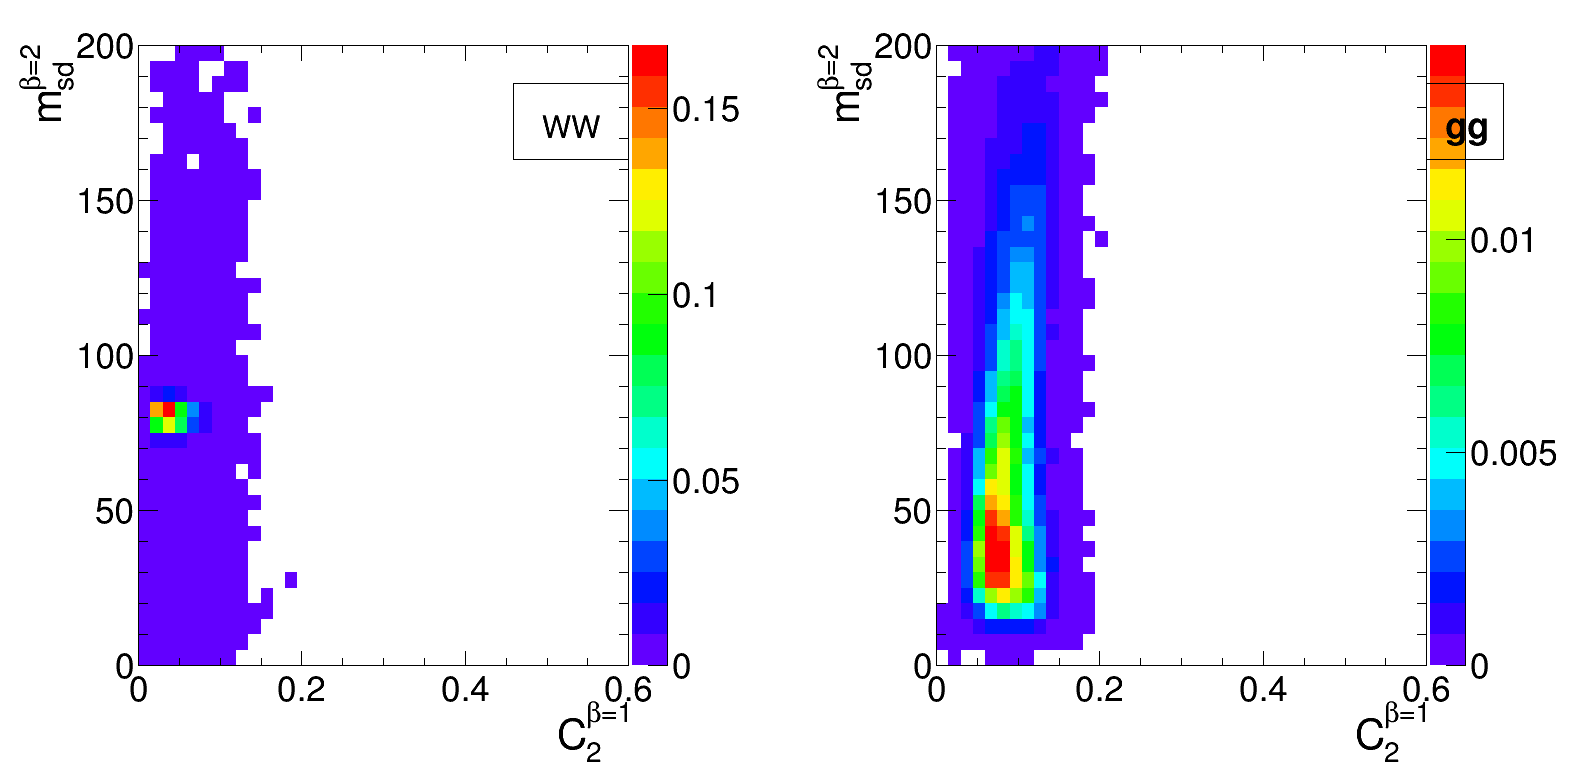
\includegraphics[width=0.78\textwidth]{./Figures/WTagging/pT1000/AKtR04/h2d_jc2_b1_j_mass_sdb2_WW_onSame.png}\label{fig:pt1000_2d_c2b1_AKt_R04}}
\subfigure[\pt R=0.8]{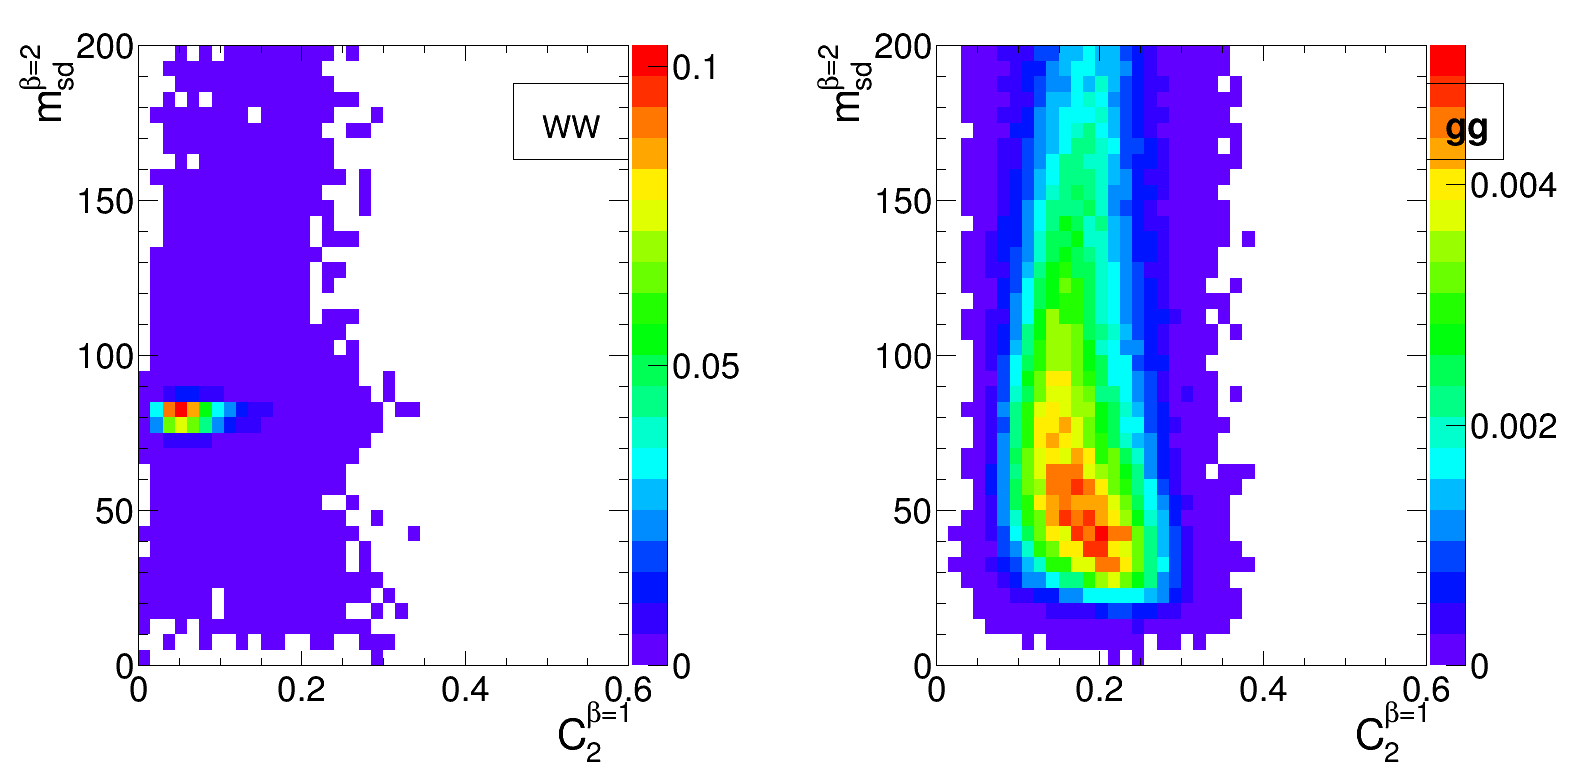
\includegraphics[width=0.78\textwidth]{./Figures/WTagging/pT1000/AKtR08/h2d_jc2_b1_j_mass_sdb2_WW_onSame.png}\label{fig:pt1000_2d_c2b1_AKt_R08_b}}
\subfigure[\pt R=1.2]{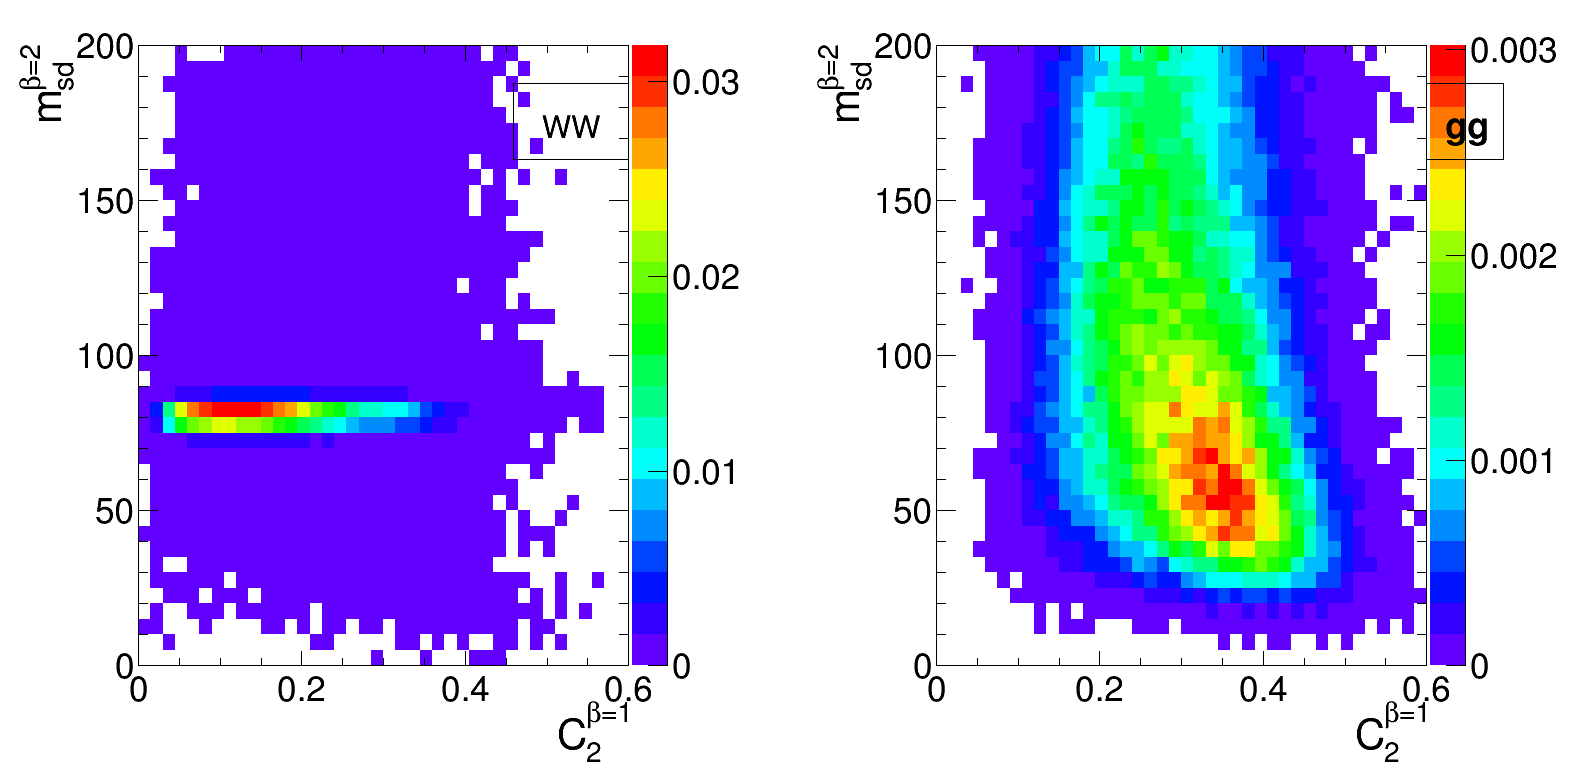
\includegraphics[width=0.78\textwidth]{./Figures/WTagging/pT1000/AKtR12/h2d_jc2_b1_j_mass_sdb2_WW_onSame.png}\label{fig:pt1000_2d_c2b1_AKt_R12}}
\caption{2-D plots showing $m_{sd}^{\beta=2}$ versus $C_2^{\beta=1}$
  for R=0.4, 0.8 and 1.2 jets in the \pt~1.0-1.1 TeV bin.}
\label{fig:2d_c2b1_pt1000}
\end{center}
\end{figure*}

\begin{figure*}
\begin{center}
\subfigure[\pt R=0.4]{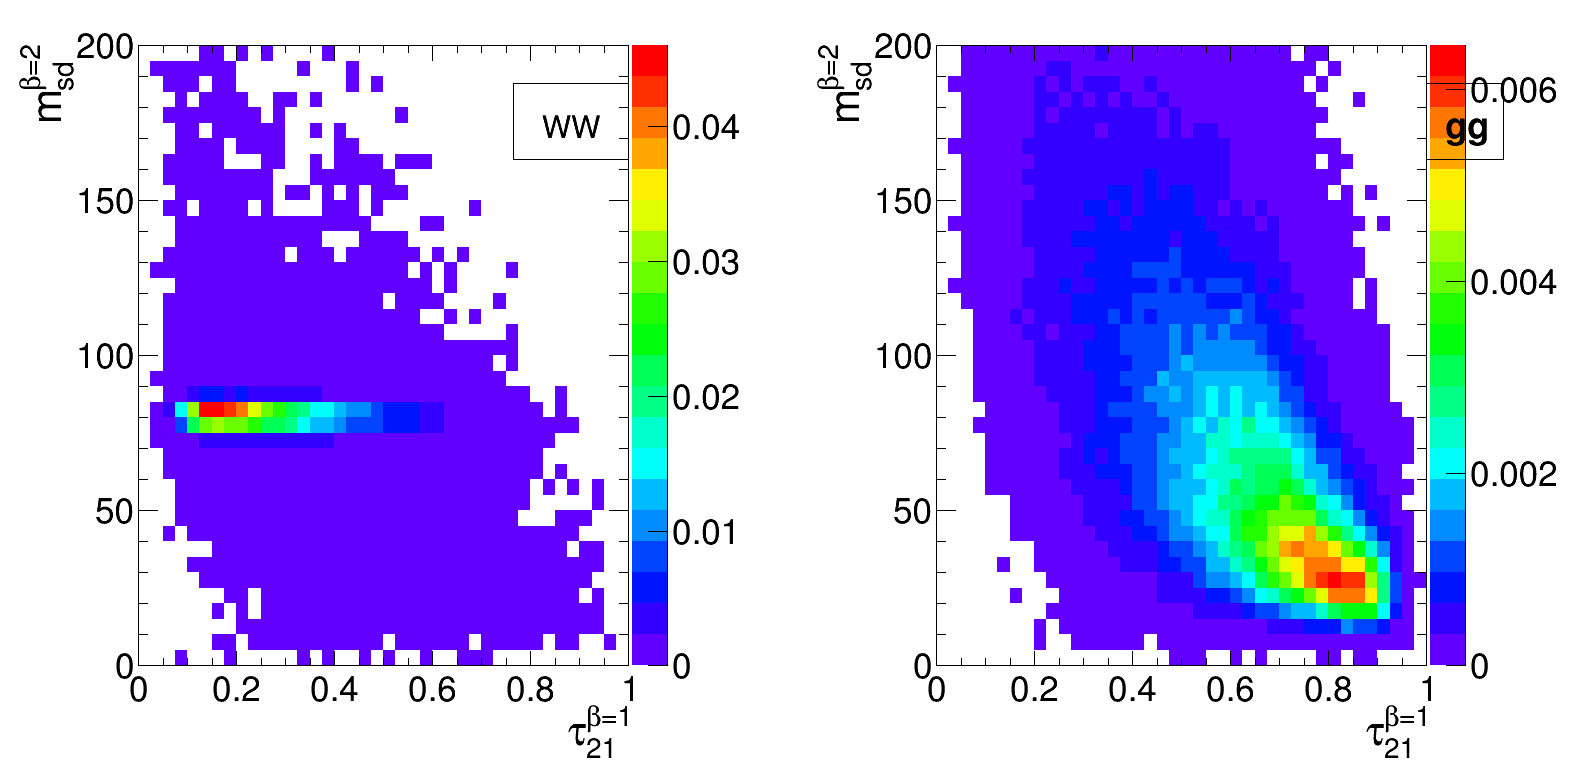
\includegraphics[width=0.78\textwidth]{./Figures/WTagging/pT1000/AKtR04/h2d_jtau21_b1_j_mass_sdb2_WW_onSame.png}\label{fig:pt1000_2d_tau21_AKt_R04}}
\subfigure[\pt R=0.8]{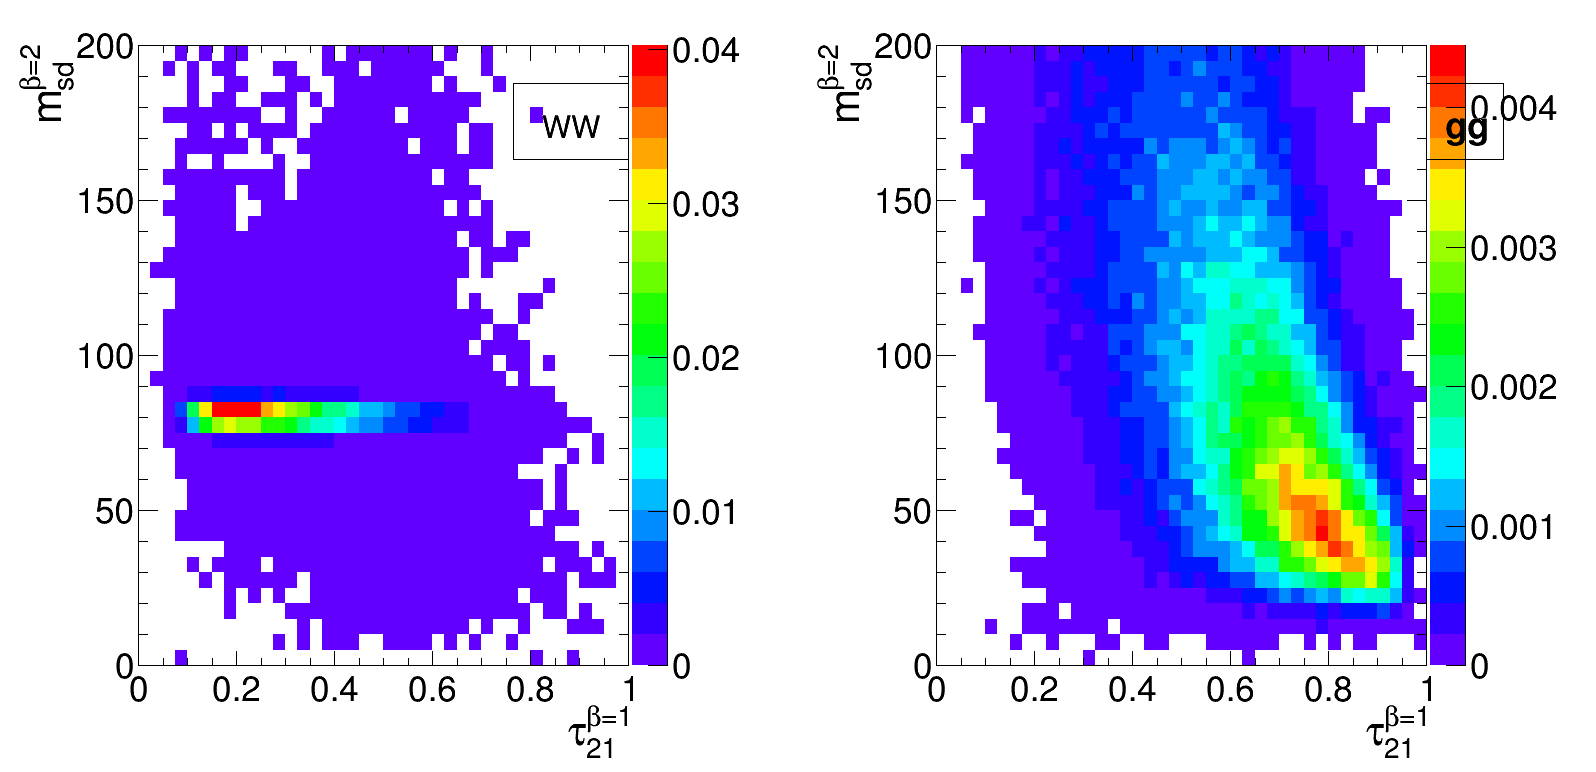
\includegraphics[width=0.78\textwidth]{./Figures/WTagging/pT1000/AKtR08/h2d_jtau21_b1_j_mass_sdb2_WW_onSame.png}\label{fig:pt1000_2d_tau21_AKt_R08_b}}
\subfigure[\pt R=1.2]{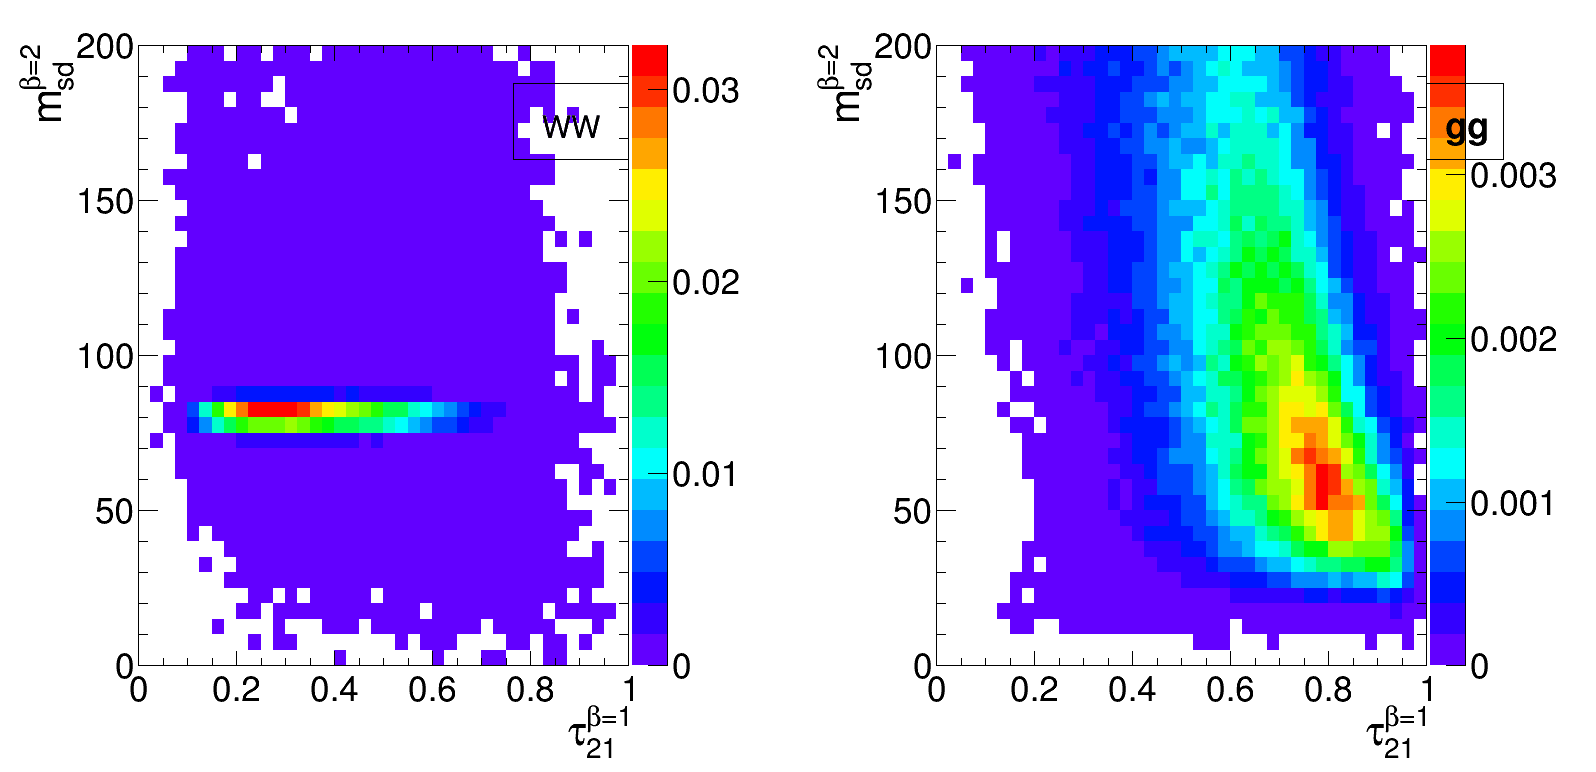
\includegraphics[width=0.78\textwidth]{./Figures/WTagging/pT1000/AKtR12/h2d_jtau21_b1_j_mass_sdb2_WW_onSame.png}\label{fig:pt1000_2d_tau21_AKt_R12}}
\caption{2-D plots showing $m_{sd}^{\beta=2}$ versus $\tau_{21}^{\beta=1}$
  for R=0.4, 0.8 and 1.2 jets in the \pt~1.0-1.1 TeV bin.}
\label{fig:2d_tau21_pt1000}
\end{center}
\end{figure*}





\subsubsection{Mass + Mass Performance}

The different groomed masses and the ungroomed mass are of course not
fully correlated, and thus one can always see some kind of improvement
in the background rejection (relative to the single mass performance) when two different mass variables are combined
in the BDT. However, in some cases the improvement can be dramatic,
particularly at higher \pt, and particularly for combinations with the
ungroomed mass. For example, in Figure~\ref{fig:pt1000_comb2D} we can
see that in the \pt~1.0-1.1 TeV bin the combination of pruned mass with
ungroomed mass produces a greater than eight-fold improvement in the
background rejection for R=0.4 jets, a greater than five-fold
improvement for R=0.8 jets, and a factor $\sim$two improvement for
R=1.2 jets. A similar behaviour can be seen for mMDT mass. 
In Figures~\ref{fig:pt1000_2d_masses_AKt_R04},~\ref{fig:pt1000_2d_masses_AKt_R08}
and~\ref{fig:pt1000_2d_masses_AKt_R12} is shown the 2-D correlation plots of the pruned mass versus the
ungroomed mass separately for the WW signal and $gg$ background
samples in the \pt~1.0-1.1 TeV bin, for the various jet radii
considered. For comparison, the correlation of the trimmed mass with
the ungroomed mass, a combination that does not improve on the single
mass as dramatically, is shown. In all cases one can see that there is
a much smaller degree of correlation between the pruned mass and the
ungroomed mass in the backgrounds sample than for the trimmed mass and the ungroomed mass. This
is most obvious in Figure~\ref{fig:pt1000_2d_masses_AKt_R04}, where
the high degree of correlation between the trimmed and ungroomed mass
is expected, since with the parameters used (in particular
$R_{trim} = 0.2$) we cannot expect trimming to have a significant
impact on an R=0.4 jet. The reduced correlation with ungroomed mass
for pruning in the background means that, once we have made the requirement that the
pruned mass is consistent with a W (i.e. $\sim$80 GeV), a relatively large difference
between signal and background in the ungroomed mass still remains, and
can be exploited to improve the background rejection further. In other
words, many of the background events which pass the pruned mass
requirement do so because they are shifted to lower mass (to be within
a signal mass window) by the grooming, but these events still have the
property that they look very much like background events before the
grooming. A single requirement on the groomed mass only does not
exploit this. Of course, the impact of pile-up, not considered in this
study, could significantly limit the degree to which the ungroomed
mass could be used to improve discrimination in this way. 

\begin{figure*}
\begin{center}
\subfigure[Pruned mass vs ungroomed mass]{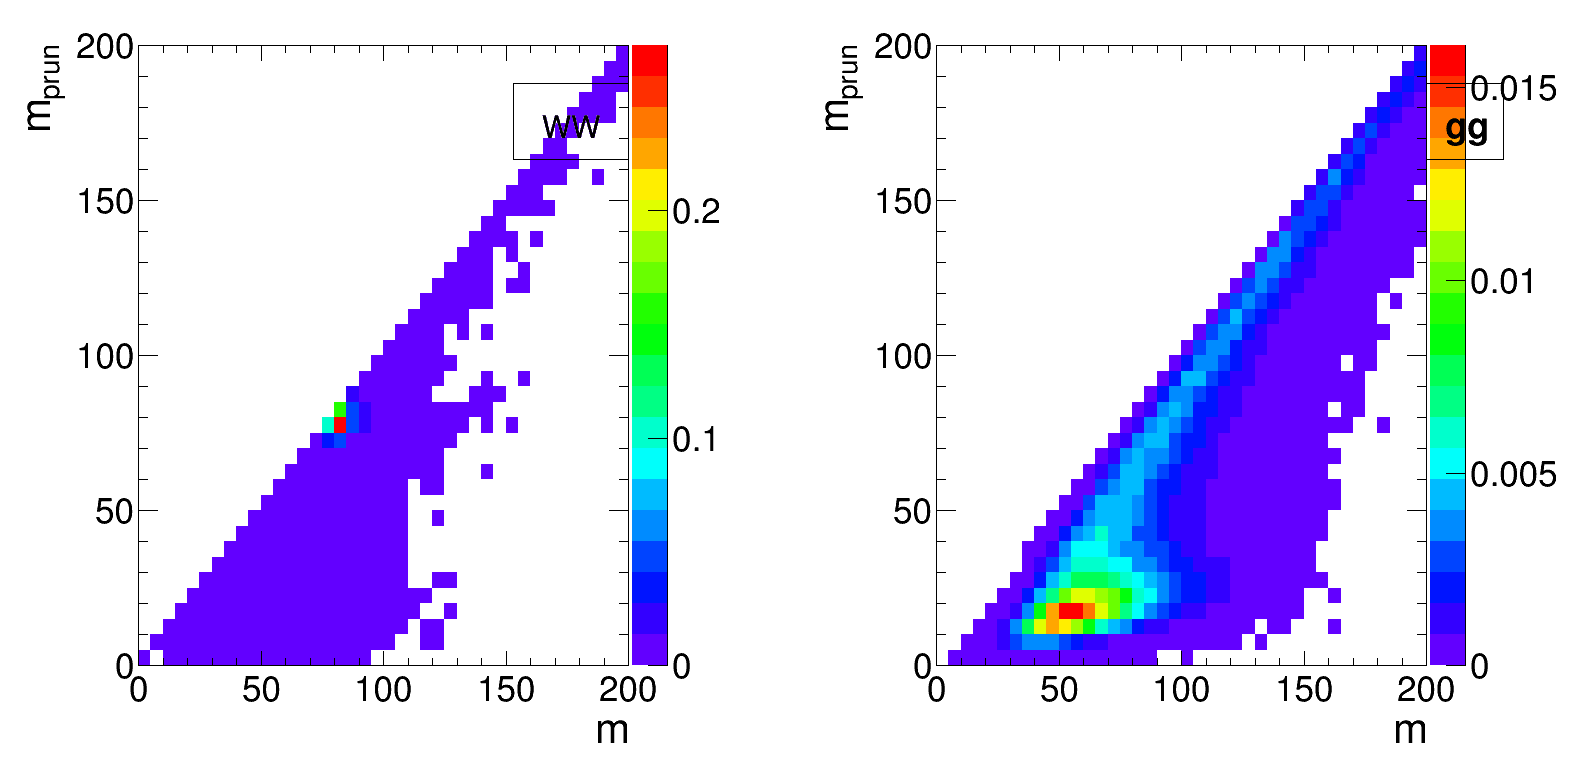
\includegraphics[width=0.78\textwidth]{./Figures/WTagging/pT1000/AKtR04/h2d_jmass_j_mass_prun_WW_onSame.png}\label{fig:pt1000_2d_prun_AKt_R04}}
\subfigure[Trimmed mass vs ungroomed mass]{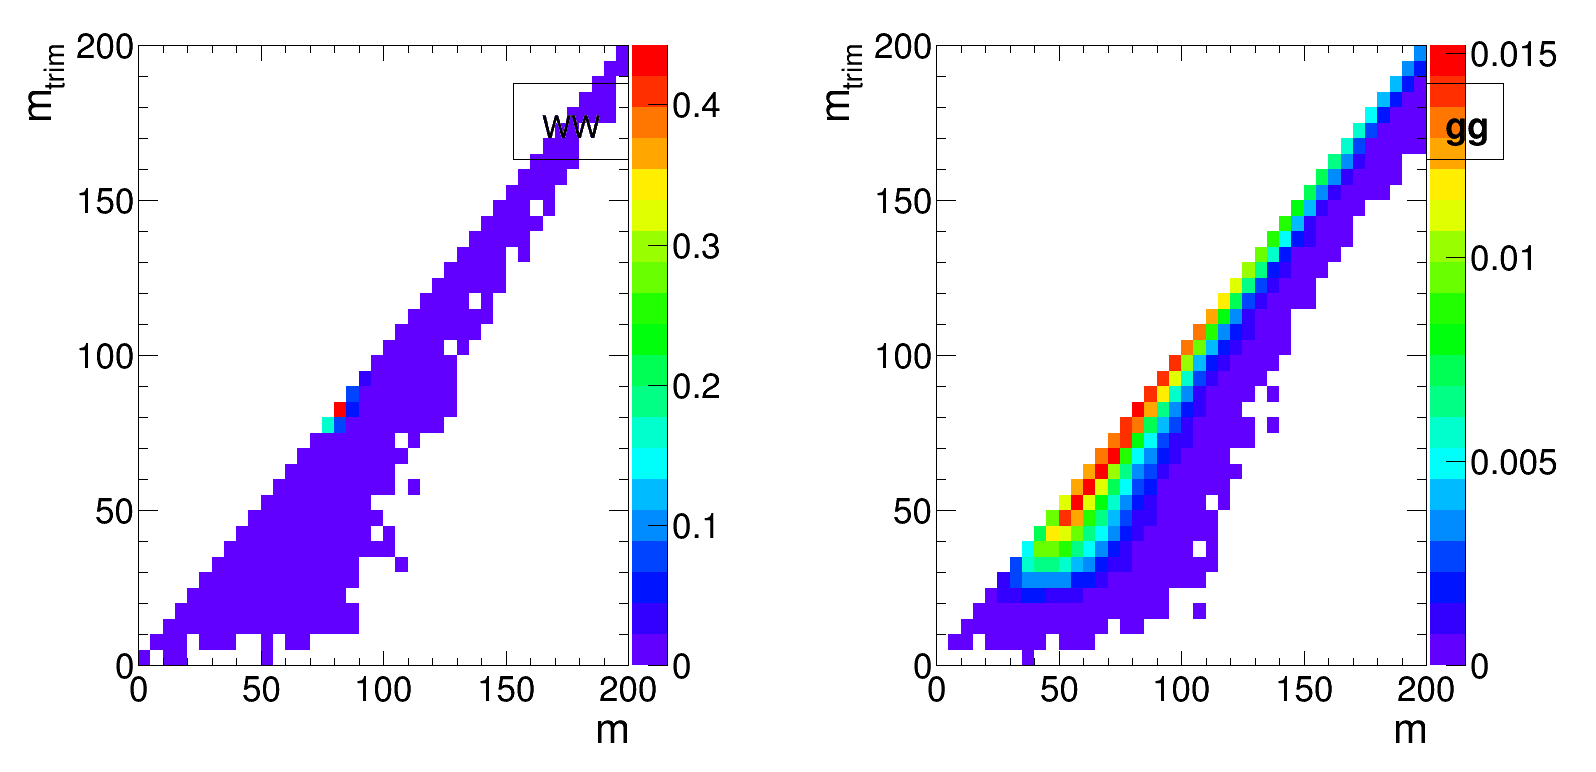
\includegraphics[width=0.78\textwidth]{./Figures/WTagging/pT1000/AKtR04/h2d_jmass_j_mass_trim_WW_onSame.png}\label{fig:pt1000_2d_trim_AKt_R04}}
\caption{2-D plots showing the correlation between groomed and
  ungroomed mass for $WW$ and $gg$ events in the \pt 1.0-1.1 TeV bin using the
  anti-\kT R=0.4 algorithm.}
\label{fig:pt1000_2d_masses_AKt_R04}
\end{center}
\end{figure*}

\begin{figure*}
\begin{center}
\subfigure[Pruned mass vs ungroomed mass]{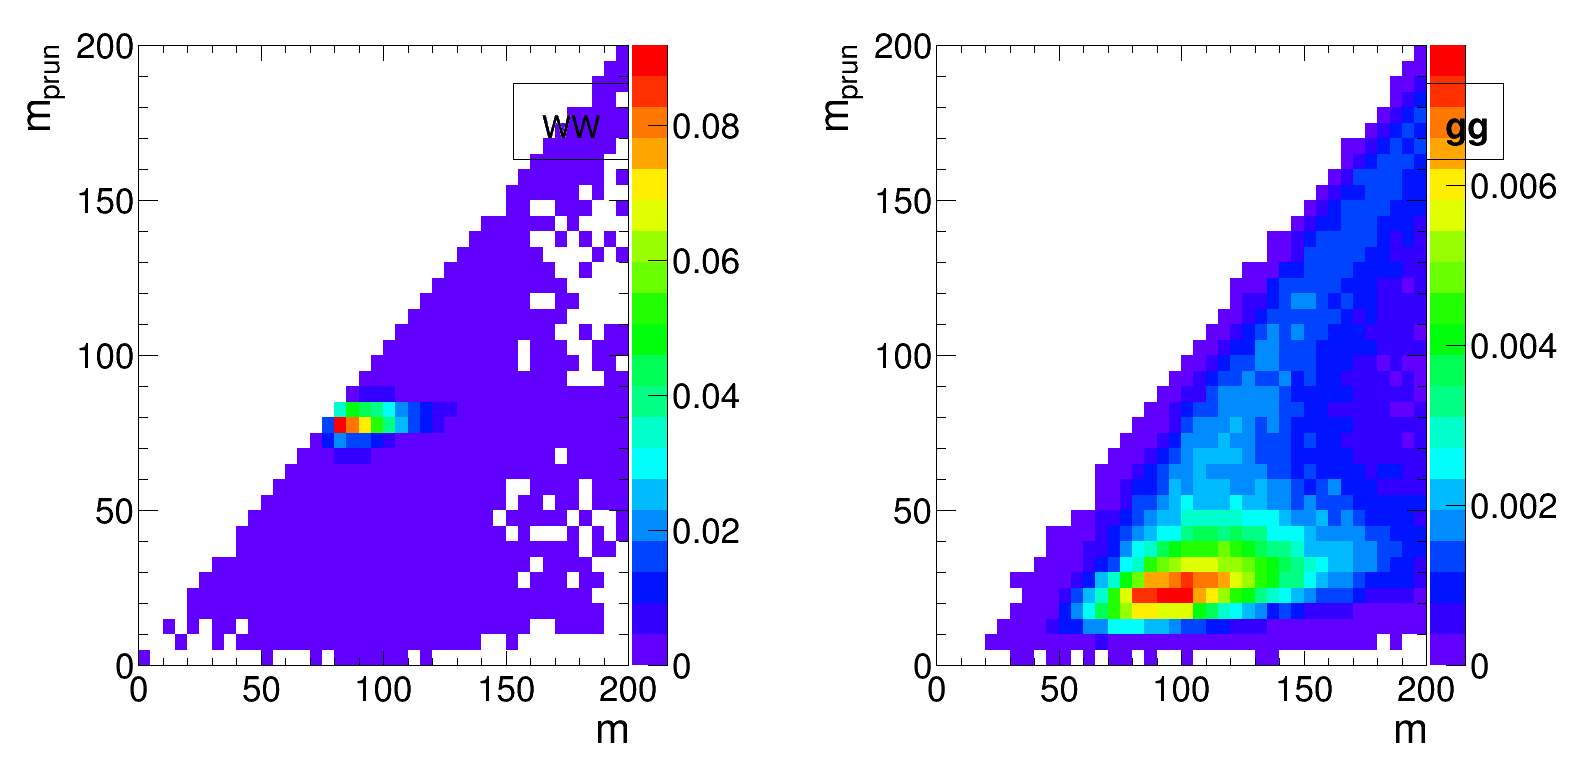
\includegraphics[width=0.78\textwidth]{./Figures/WTagging/pT1000/AKtR08/h2d_jmass_j_mass_prun_WW_onSame.png}\label{fig:pt1000_2d_prun_AKt_R08}}
\subfigure[Trimmed mass vs ungroomed mass]{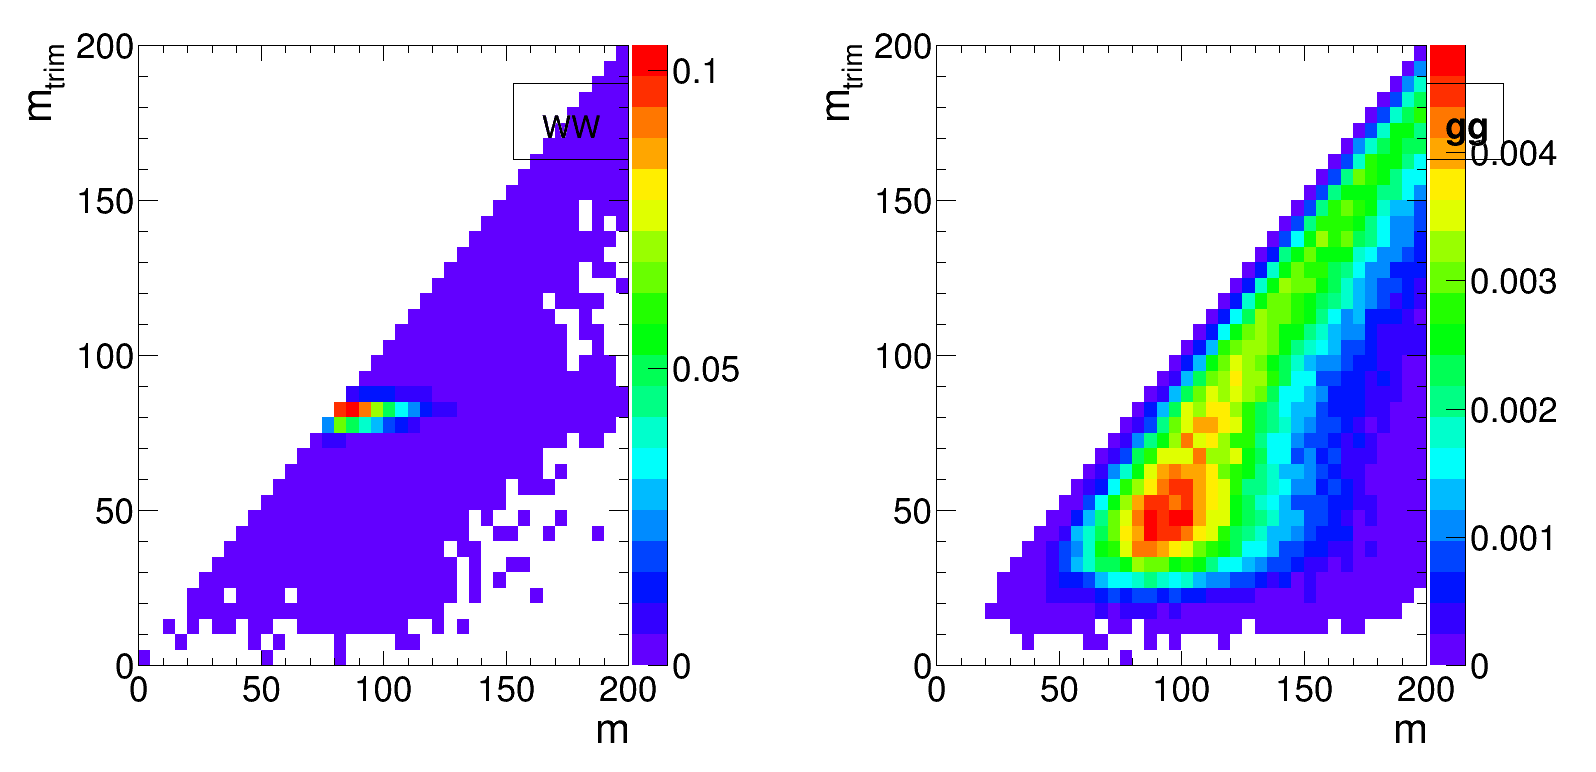
\includegraphics[width=0.78\textwidth]{./Figures/WTagging/pT1000/AKtR08/h2d_jmass_j_mass_trim_WW_onSame.png}\label{fig:pt1000_2d_trim_AKt_R08}}
\caption{2-D plots showing the correlation between groomed and
  ungroomed mass for $WW$ and $gg$ events in the \pt 1.0-1.1 TeV bin using the
  anti-\kT R=0.8 algorithm.}
\label{fig:pt1000_2d_masses_AKt_R08}
\end{center}
\end{figure*}

\begin{figure*}
\begin{center}
\subfigure[Pruned mass vs ungroomed mass]{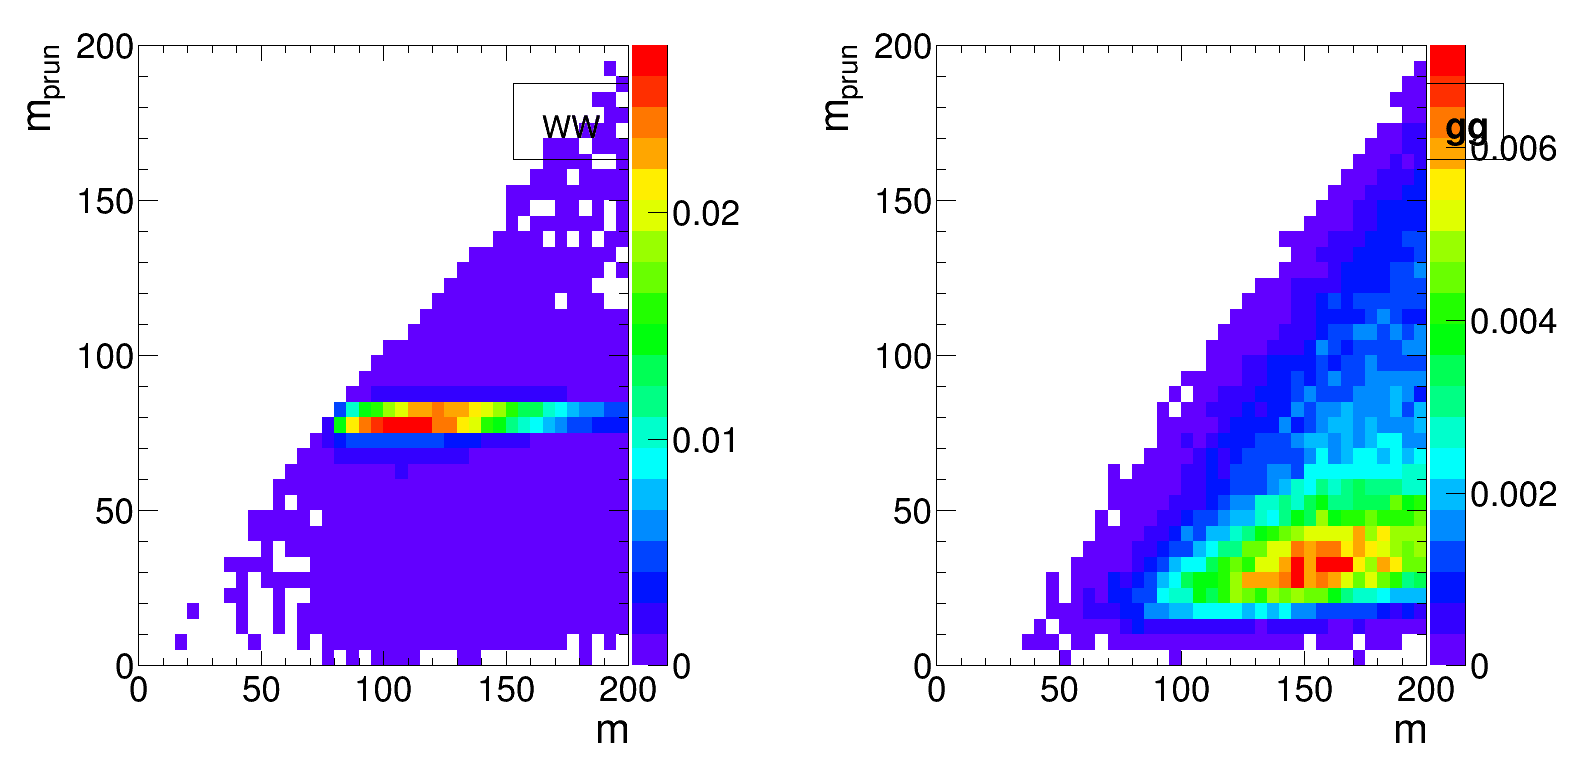
\includegraphics[width=0.78\textwidth]{./Figures/WTagging/pT1000/AKtR12/h2d_jmass_j_mass_prun_WW_onSame.png}\label{fig:pt1000_2d_prun_AKt_R12}}
\subfigure[Trimmed mass vs ungroomed mass]{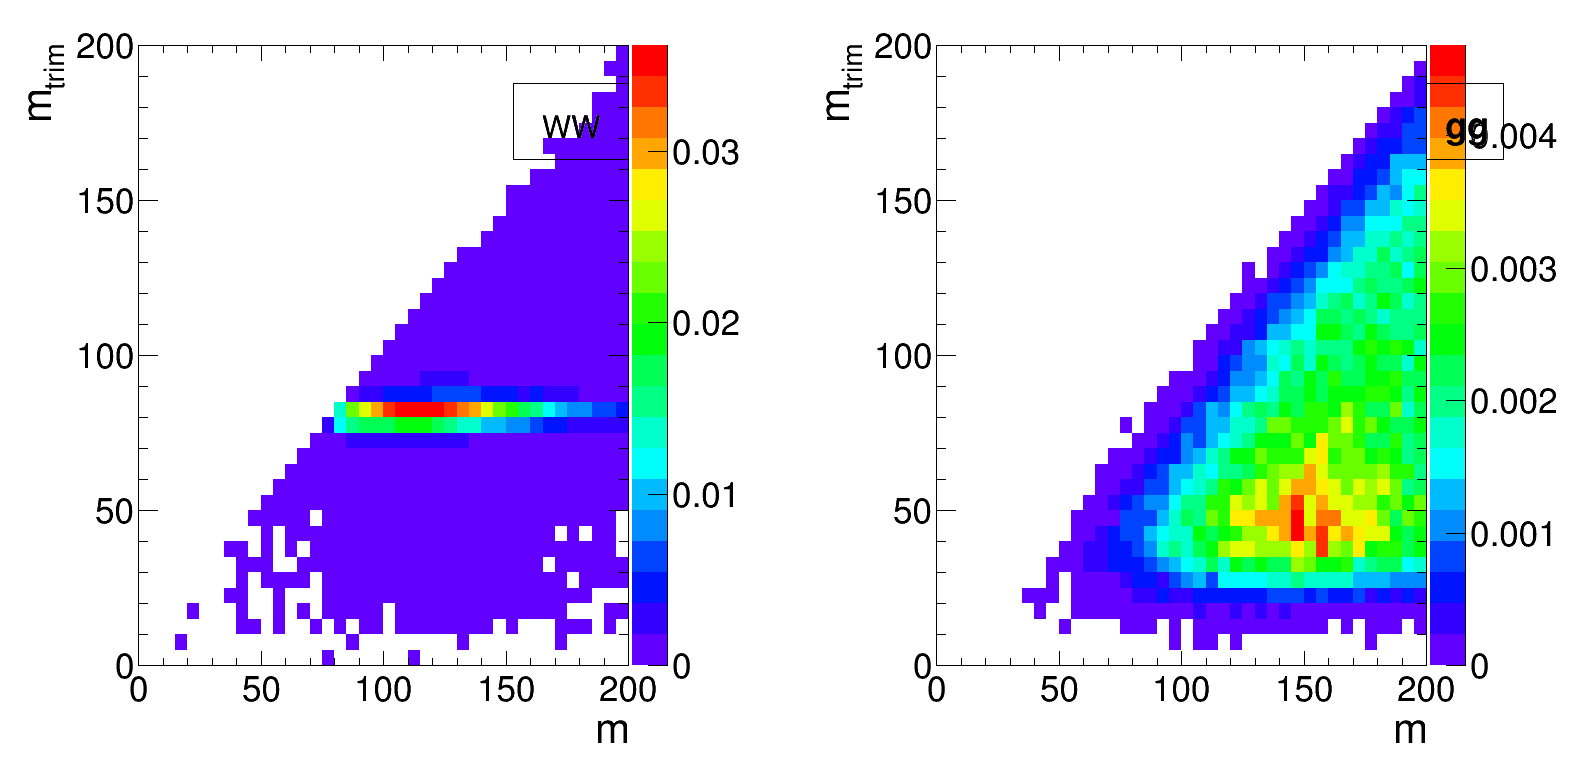
\includegraphics[width=0.78\textwidth]{./Figures/WTagging/pT1000/AKtR12/h2d_jmass_j_mass_trim_WW_onSame.png}\label{fig:pt1000_2d_trim_AKt_R12}}
\caption{2-D plots showing the correlation between groomed and
  ungroomed mass for $WW$ and $gg$ events in the \pt 1.0-1.1 TeV bin using the
  anti-\kT R=1.2 algorithm.}
\label{fig:pt1000_2d_masses_AKt_R12}
\end{center}
\end{figure*}

\subsubsection{``All Variables'' Performance}\label{sec:Wtagallvars}

As well as the background rejection at a fixed 70\% signal efficiency
for two-variable combinations, Figures~\ref{fig:pt300_comb2D},~\ref{fig:pt500_comb2D}
and~\ref{fig:pt1000_comb2D} also report the background rejection
achieved by a combination of all the variables considered into a
single BDT discriminant. One can see that, in all cases, the rejection
power of this ``all variables'' BDT is significantly larger than the
best two-variable combination. This indicates
that beyond the best two-variable combination there is still
significant complementary information availiable in the remaining
variables in order to improve the discrimination of signal and
background. How much complementary information is available appears to
be \pt dependent. In the lower \pt 300-400 and 500-600 GeV bins the
background rejection of the ``all variables'' combination is a factor
$\sim 1.5$ greater than the best two-variable combination, but in the
highest \pt bin it is a factor $\sim 2.5$ greater. 

The final column in Figures ~\ref{fig:pt300_comb2D},~\ref{fig:pt500_comb2D}
and~\ref{fig:pt1000_comb2D} allows us to explore the all variables
performance a little further. It shows the background rejection for 
three variable BDT combinations of $m_{sd}^{\beta=2} + C_2^{\beta=1} +
X$, where $X$ is the variable on the y-axis. For jets with R=0.4 and
R=0.8, the combination $m_{sd}^{\beta=2} + C_2^{\beta=1}$
is the best performant (or very close to the best performant)
two-variable combination in every \pt bin considered. For R=1.2 this
is not the case, as $C_2^{\beta=1}$ is superceded by
$\tau_{21}^{\beta=1}$ in performance, as discussed earlier. Thus, in
considering the three-variable combination results it is best to focus
on the R=0.4 and R=0.8 cases. Here we see that, for the lower \pt
300-400 and 500-600 GeV bins, adding the third variable to the best
two-variable combination brings us to within $\sim 15\%$ of the ``all
variables'' background rejection. However, in the highest \pt 1.0-1.1 TeV bin, whilst adding the third
variable does improve the performance considerably, we are still $\sim
40\%$ from the observed ``all variables'' background rejection, and
clearly adding a fourth or maybe even fifth variable would bring
considerable gains. In terms of which variable offers the best
improvement when added to the $m_{sd}^{\beta=2} + C_2^{\beta=1}$
combination, it is hard to see an obvious pattern; the best third
variable changes depending on the \pt and R considered.

In conclusion, it appears that there is a rich and
complex structure in terms of the degree to which the discriminatory
information provided by the set of variables considered overlaps, with
the degree of overlap apparently decreasing at higher \pt. This
suggests that in all \pt ranges, but especially at higher \pt, there
are substantial performance gains to be made by designing a more
complex multivariate W tagger.

\subsection{Conclusions}

We have studied the performance, in terms of the degree to which a
hadronically decaying W boson can be separated from a gluonic
background, of a number of groomed jet masses, substructure variables,
and BDT combinations of the above. We have used this to build a
picture of how the discriminatory information contained in the
variables overlaps, and how this complementarity between the variables
changes with \pt and \antikt distance parameter R. 

In terms of the performance of individual variables, we find that, in
agreement with other studies\refneeded, in
general the groomed masses perform best, with a background rejection
power that increases with increasing \pt, but which is more constant
with respect to changes in R. Conversely, the performance of other
substructure variables, such as $C_2^{\beta=1}$ and
$\tau_{21}^{\beta=1}$ is more susceptible to changes in radius, with
background rejection power decreasing with increasing R.

The best two-variable performance is obtained by combining a groomed
mass with a substructure variable. Which particular substructure
variable works best in combination is strongly dependent on \pt and
R. $C_2^{\beta=1}$ offers significant complimentarity to groomed mass
at smaller R, owing to the small degree of correlation between the
variables. However, the sensitivity of $C_2^{\beta=1}$ to soft,
wide-angle radiation leads to worse discrimination power at large R,
where $\tau_{21}^{\beta=1}$ performs better in combination. Our
studies also demonstrate the potential for enhanced discrmination by
combining groomed and ungroomed mass information, although the use of
ungroomed mass in this may in practice be limited by the presence of
pile-up that is not considered in these studies.

By examining the performance of a BDT combination of all the variables
considered, it is clear that there are potentially substantial performance gains to be made by designing a more
complex multivariate W tagger, especially at higher \pt.




%\subsubsection*{Mass + X Performance}
%
%Figure~\ref{fig:pt500_2Dcomb_AKt_R08} shows the background efficiency
%for a fixed signal efficiency (50\%) of each BDT combination of
%each pair of variables considered, in the \pt 500 GeV bin using the anti-\kT R=0.8
%algorithm. One can see that the best background rejection is achieved
%using combinations of the groomed mass variables with other
%substructure variables (with the exception
%of the soft drop mass with $\beta=-1$). Combinations of the mass
%variables themselves are not particularly powerful, but are
%interesting for understanding the correlations between the masses (see
%Section~\ref{sec:wtag_massplusmass}). Equally, combination of the
%substructure variables, without using a mass, are not powerful. 
%
%Figure~\ref{fig:pt500_masscomb_AKt_R08} shows the actual ROC curves of the BDT combinations of each mass variable with every other
%variable considered in the \pt 500 GeV bin using the anti-\kT R=0.8
%algorithm. {\it Can we drop the combinations of mass + mass
%from these plots to make them clearer? Also would be good to put the
%single variable mass curve on these plots, so you can see how much
%improvement the combination gives, and the ``all variables'' curve.}
%
%No combination with other variables can recover the poor performance
%of the ungroomed mass and the soft drop mass with
%$\beta=-1$. Figures~\ref{fig:pt500_2Dcomb_AKt_R08}
%and~\ref{fig:pt500_masscomb_AKt_R08} show that the
%other groomed/filtered masses are all most improved by combination
%with the $C_{2}^{\beta=1}$ energy correlation
%function. Figure~\ref{fig:pt500_2d_mmdt_AKt_R08} shows the 2-D
%correlation plots between the mMDT mass and the $C_{2}^{\beta=1}$,
%$\Gamma_{Qjet}$ and $\tau_{21}^{\beta=1}$ variables. One can clearly
%see that there is substantially less correlation between the mass and
%$C_{2}^{\beta=1}$ than the other variables. Similar results are seen
%for the other groomed masses.
%
%\begin{figure*}
%\begin{center}
%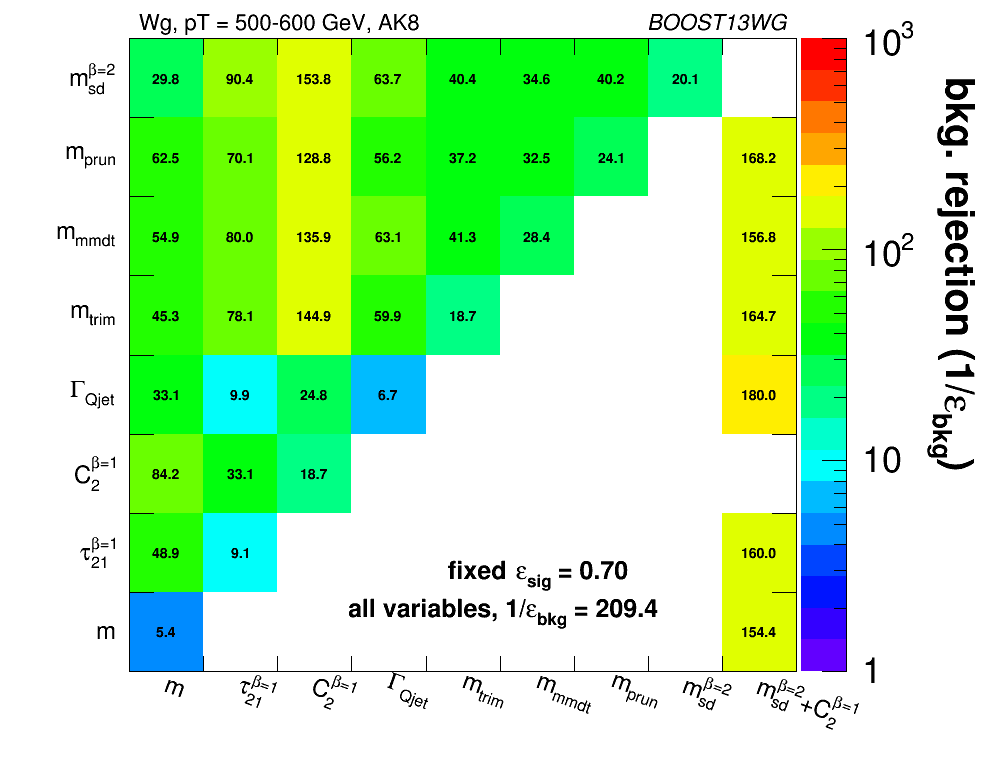
\includegraphics[width=0.48\textwidth]{./Figures/WTagging/pT500/AKtR08/effBkg2D.png}
%\caption{The background efficiency
%for a fixed signal efficiency (50\%) of each BDT combination of
%each pair of variables considered, in the \pt 500 GeV bin using the anti-\kT R=0.8
%algorithm.}
%\label{fig:pt500_2Dcomb_AKt_R08}
%\end{center}
%\end{figure*}
%
%
%\begin{figure*}
%\begin{center}
%\subfigure[Ungroomed mass + X]{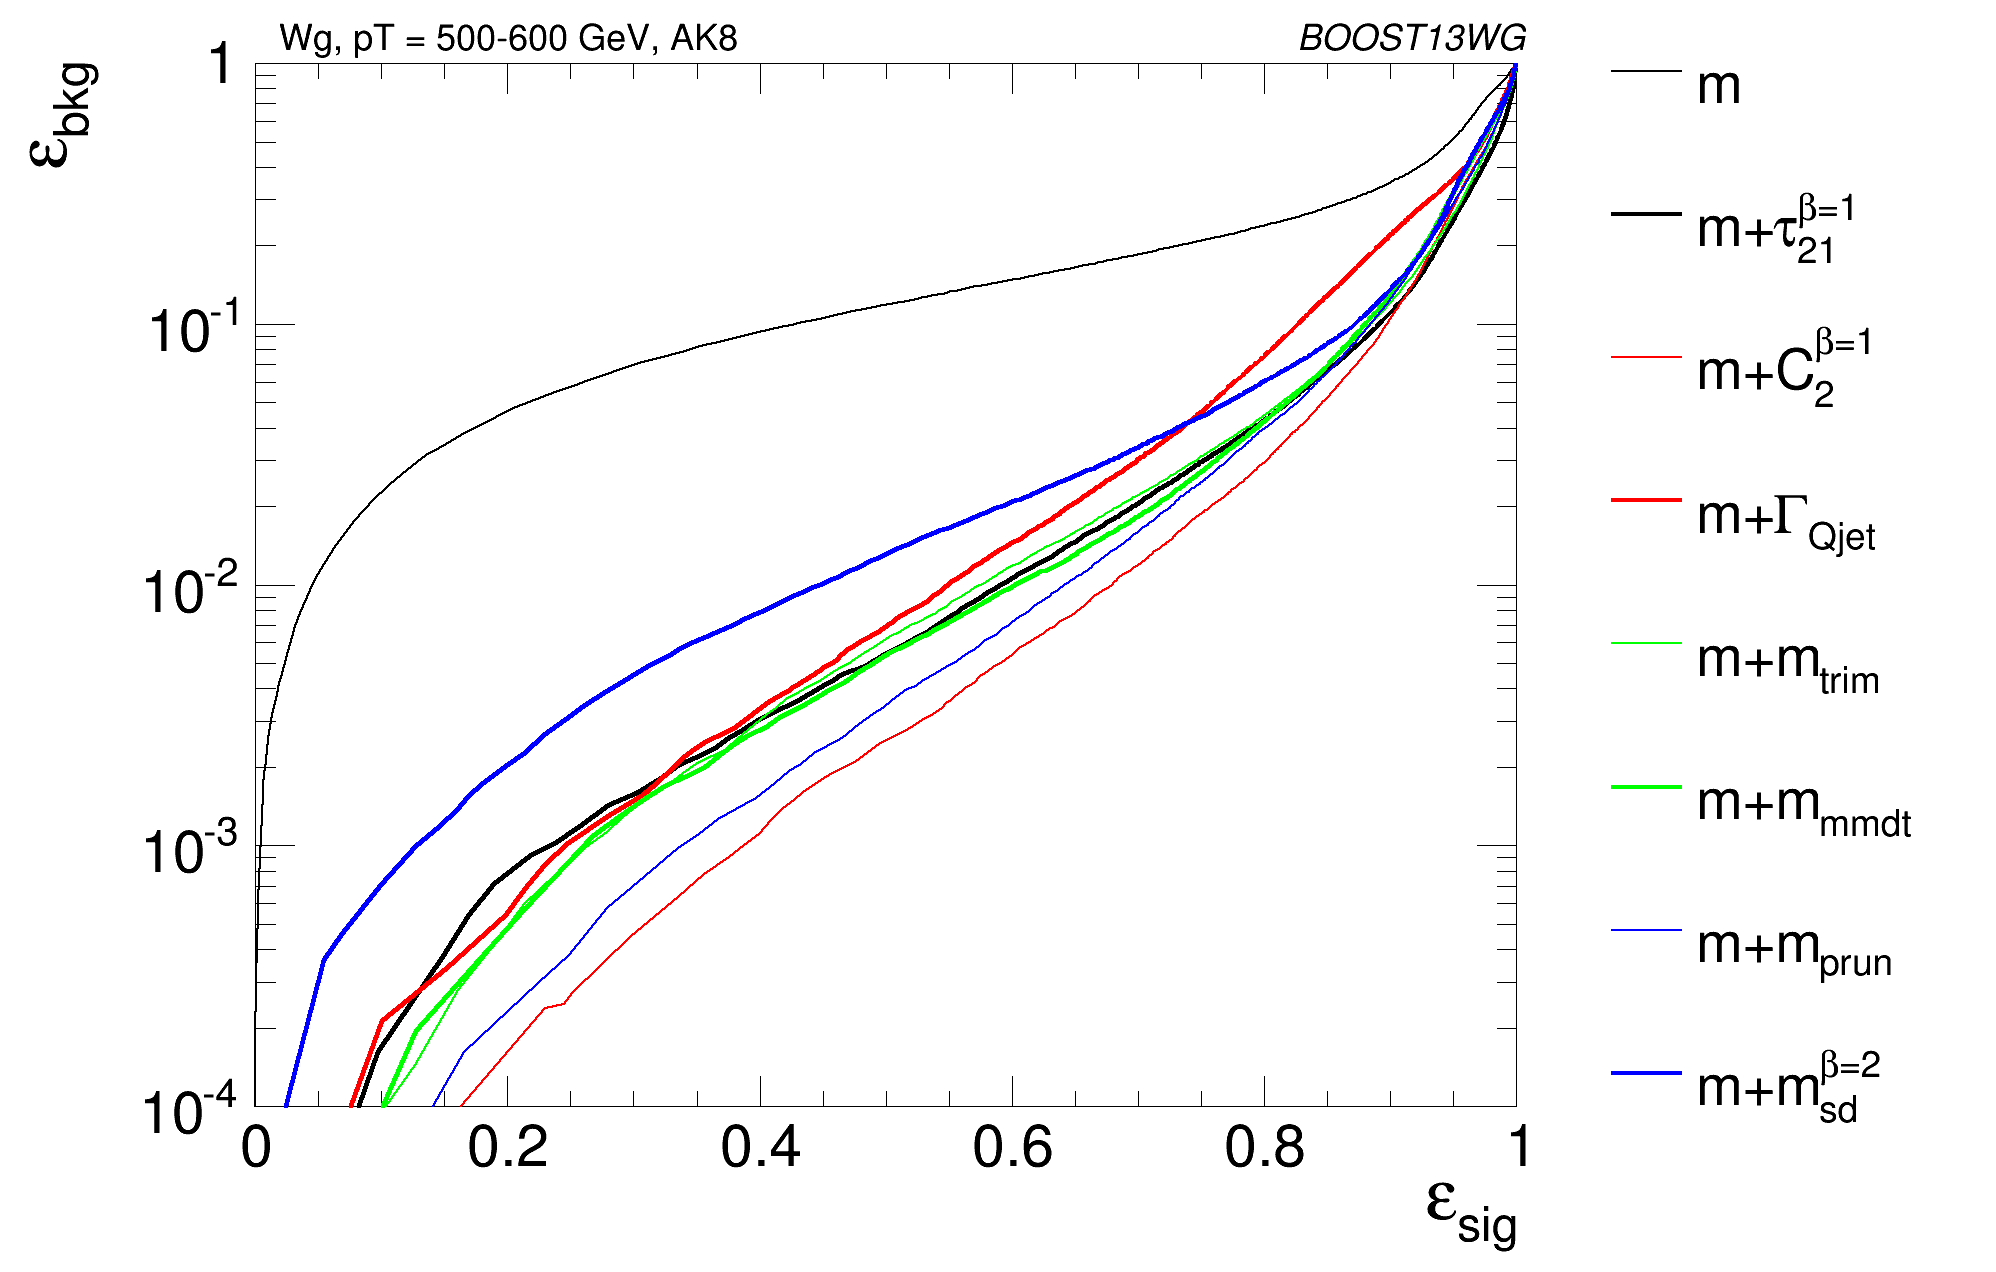
\includegraphics[width=0.48\textwidth]{./Figures/WTagging/pT500/AKtR08/Rocs_1D_jmass.png}}
%\subfigure[Trimmed mass + X]{\includegraphics[width=0.48\textwidth]{./Figures/WTagging/pT500/AKtR08/Rocs_1D_j_mass_trim.png}}
%\subfigure[Pruned mass + X]{\includegraphics[width=0.48\textwidth]{./Figures/WTagging/pT500/AKtR08/Rocs_1D_j_mass_prun.png}}
%%\subfigure[Soft drop mass ($\beta=-1$) +X]{\includegraphics[width=0.48\textwidth]{./Figures/WTagging/pT500/AKtR08/Rocs_1D_j_mass_sdm1.png}}
%\subfigure[Soft drop mass ($\beta=2$) + X]{\includegraphics[width=0.48\textwidth]{./Figures/WTagging/pT500/AKtR08/Rocs_1D_j_mass_sdb2.png}}
%\subfigure[mMDT mass + X]{\includegraphics[width=0.48\textwidth]{./Figures/WTagging/pT500/AKtR08/Rocs_1D_j_mass_mmdt.png}}
%\caption{The BDT combinations of each mass variable with every other
%variable considered in the \pt 500 GeV bin using the anti-\kT R=0.8 algorithm.}
%\label{fig:pt500_masscomb_AKt_R08}
%\end{center}
%\end{figure*}
%
%
%\begin{figure*}
%\begin{center}
%\subfigure[mMDT mass vs $C_2^{\beta=1}$]{\includegraphics[width=0.48\textwidth]{./Figures/figs072514/figs071614_Wg_bin500_ak08/twoD/h2d_jc2_b1_j_mass_mmdt_gg.png}}
%\subfigure[mMDT mass vs $\Gamma_{Qjet}$]{\includegraphics[width=0.48\textwidth]{./Figures/figs072514/figs071614_Wg_bin500_ak08/twoD/h2d_j_qjetVol_j_mass_mmdt_gg.png}}
%\subfigure[mMDT mass vs $\tau_{21}^{\beta=1}$]{\includegraphics[width=0.48\textwidth]{./Figures/figs072514/figs071614_Wg_bin500_ak08/twoD/h2d_jtau21_b1_j_mass_mmdt_gg.png}}
%\caption{2-D plots showing the correlation between mMDT mass and
%  various substructure variables in the \pt 500 GeV bin using the
%  anti-\kT R=0.8 algorithm in the gg sample.}
%\label{fig:pt500_2d_mmdt_AKt_R08}
%\end{center}
%\end{figure*}
%
%Figure~\ref{fig:pt500_2Dcomb_AKt_R12} shows the background efficiency
%for a fixed signal efficiency (50\%) of each BDT combination of
%each pair of variables considered, in the \pt 500 GeV bin, now using the anti-\kT R=1.2
%algorithm. Compared to Figure~\ref{fig:pt500_2Dcomb_AKt_R08}, the
%overall trends are similar, but there are clear differences in the
%relative power of the mass + X combinations. Interestingly, the groomed masses are now all most improved by combination
%with the $\tau_{21}^{\beta=1}$ variable, in contrast with
%$C_{2}^{\beta=1}$ which performed best for the smaller radius of
%R=0.8. 
%%Q-jet volatility also performs markedly better than it did in
%%the R=0.8 case. 
%Figure~\ref{fig:pt500_masscomb_AKt_R12} shows the actual ROC curves
%for the BDT combinations of
%the best performant groomed masses with every other
%variable considered in the \pt 500 GeV bin using the anti-\kT R=1.2
%algorithm. 
%%Interestingly, the groomed masses are now all most improved by combination
%%with the $\tau_{21}^{\beta=1}$ variable, in contrast with
%%$C_{2}^{\beta=1}$ which performed best for the smaller radius of
%%R=0.8. 
%One can see from Figure~\ref{fig:pt500_single_AKt_R12} that the
%single variable discrimination of $\tau_{21}^{\beta=1}$ and
%$C_{2}^{\beta=1}$ changes quite markedly when the distance parameter R
%is varied, although in both cases $C_{2}^{\beta=1}$ is a better single
%variable discriminant (except for very high signal
%efficiencies). Figure~\ref{fig:pt500_subst_AKt_R08_R12} shows how the
%actual distributions of the $C_{2}^{\beta=1}$ and $\tau_{21}^{\beta=1}$
%change when we change the distance parameter. Figure~\ref{fig:pt500_2d_mmdt_AKt_R12} shows the 2-D
%correlation plots between between the mMDT mass and the $C_{2}^{\beta=1}$,
%$\Gamma_{Qjet}$ and $\tau_{21}^{\beta=1}$ variables for the R=1.2
%case. It is hard to see a substantial difference in the correlations
%here versus Figure~\ref{fig:pt500_2d_mmdt_AKt_R08}, but perhaps
%$C_{2}^{\beta=1}$ is marginally more correlated with the mass for
%R=1.2 compared to R=0.8.
%{\it Andrew to add his explanation of why discrimination power of C2 versus tau21
%  gets worse when we go to larger jet radii (email 0606/2014)}
%
%
%{\it Now show a plot which compares on one plot the best combined performance for
%each groomed mass + X for both R=0.8 and 1.2 cases e.g. mass +
%$C_{2}^{\beta=1}$ for R=0.8 and mass + $\tau_{21}^{\beta=1}$ for R=1.2,
%  and draw on also the
%all variables curve for both R=0.8,1.2. 
%Then we can see if there is much dependence on choice of mass once you
%combine with another variable, and compare directly the two distance parameters.
%This plot is just for
%one kinematic bin, we should make the same plot for others.}
%
%{\it Repeat these studies for different R and different kinematic
%bins. Finally make plots which compare best combined performance for
%different R and kinematics.}
%
%{\it Do we want to look at other combinations of variables which don't
%involve mass? Practically I think we will always be making mass + X though.}
%
%
%\begin{figure*}
%\begin{center}
%\includegraphics[width=0.48\textwidth]{./Figures/WTagging/pT500/AKtR12/effBkg2D.png}
%\caption{The background efficiency
%for a fixed signal efficiency (50\%) of each BDT combination of
%each pair of variables considered, in the \pt 500 GeV bin using the anti-\kT R=1.2
%algorithm.}
%\label{fig:pt500_2Dcomb_AKt_R12}
%\end{center}
%\end{figure*}
%
%\begin{figure*}
%\begin{center}
%%\subfigure[Ungroomed mass + X]{\includegraphics[width=0.48\textwidth]{./Figures/WTagging/pT500/AKtR12/Rocs_1D_jmass.png}}
%\subfigure[Trimmed mass + X]{\includegraphics[width=0.48\textwidth]{./Figures/WTagging/pT500/AKtR12/Rocs_1D_j_mass_trim.png}}
%\subfigure[Pruned mass + X]{\includegraphics[width=0.48\textwidth]{./Figures/WTagging/pT500/AKtR12/Rocs_1D_j_mass_prun.png}}
%%\subfigure[Soft drop mass ($\beta=-1$) +X]{\includegraphics[width=0.48\textwidth]{./Figures/WTagging/pT500/AKtR12/Rocs_1D_j_mass_sdm1.png}}
%\subfigure[Soft drop mass ($\beta=2$) + X]{\includegraphics[width=0.48\textwidth]{./Figures/WTagging/pT500/AKtR12/Rocs_1D_j_mass_sdb2.png}}
%\subfigure[mMDT mass + X]{\includegraphics[width=0.48\textwidth]{./Figures/WTagging/pT500/AKtR12/Rocs_1D_j_mass_mmdt.png}}
%\caption{The BDT combinations of each mass variable with every other
%variable considered in the \pt 500 GeV bin using the anti-\kT R=1.2 algorithm.}
%\label{fig:pt500_masscomb_AKt_R12}
%\end{center}
%\end{figure*}
%
%\begin{figure*}
%\begin{center}
%\subfigure[$C_2^{\beta=1}$, R=0.8]{\includegraphics[width=0.48\textwidth]{./Figures/WTagging/pT500/AKtR08/h_c2_b1.png}}
%\subfigure[$C_2^{\beta=1}$, R=1.2]{\includegraphics[width=0.48\textwidth]{./Figures/WTagging/pT500/AKtR12/h_c2_b1.png}}
%\subfigure[$\tau_{21}^{\beta=1}$, R=0.8]{\includegraphics[width=0.48\textwidth]{./Figures/WTagging/pT500/AKtR08/h_tau21_b1.png}}
%\subfigure[$\tau_{21}^{\beta=1}$, R=1.2]{\includegraphics[width=0.48\textwidth]{./Figures/WTagging/pT500/AKtR12/h_tau21_b1.png}}
%\caption{Comparisons of the QCD background to the WW signal in the \pt
%  500 GeV bin for $C_2^{\beta=1}$ and $\tau_{21}^{\beta=1}$ variables
%  and using the R=0.8 and R=1.2 anti-\kT distance parameters.}
%\label{fig:pt500_subst_AKt_R08_R12}
%\end{center}
%\end{figure*}
%
%
%\begin{figure*}
%\begin{center}
%\subfigure[mMDT mass vs $C_2^{\beta=1}$]{\includegraphics[width=0.48\textwidth]{./Figures/figs072514/figs071614_Wg_bin500_ak12/twoD/h2d_jc2_b1_j_mass_mmdt_gg.png}}
%\subfigure[mMDT mass vs $\Gamma_{Qjet}$]{\includegraphics[width=0.48\textwidth]{./Figures/figs072514/figs071614_Wg_bin500_ak12/twoD/h2d_j_qjetVol_j_mass_mmdt_gg.png}}
%\subfigure[mMDT mass vs $\tau_{21}^{\beta=1}$]{\includegraphics[width=0.48\textwidth]{./Figures/figs072514/figs071614_Wg_bin500_ak12/twoD/h2d_jtau21_b1_j_mass_mmdt_gg.png}}
%\caption{2-D plots showing the correlation between mMDT mass and
%  various substructure variables in the \pt 500 GeV bin using the
%  anti-\kT R=1.2 algorithm in the gg sample.}
%\label{fig:pt500_2d_mmdt_AKt_R12}
%\end{center}
%\end{figure*}
%
%
%\subsubsection*{Mass + Mass Performance}
%\label{sec:wtag_massplusmass}
%It's interesting also to study and understand how the different
%groomed masses relate to each other and how they are correlated.
%
%Figures~\ref{fig:pt500_2d_massQQ_AKt_R08} and Figures~\ref{fig:pt500_2d_massGG_AKt_R08} shows 2-D correlation plots of
%the different types of groomed mass in the \pt 500 GeV bin using the anti-\kT R=0.8
%algorithm.
%
%{\it Worth also showing some ROC curves for mass + mass combinations?}
%
%
%\begin{table*}[htbp!]
%\centering
%%\setlength\fboxsep{0pt}
%%\setlength\fboxrule{0.25pt}
%\caption{Action of various groomers on the jet mass distribution in the different phase space regions.  For pruning, $a_\text{prune} = \zcut R_0$ and for trimming $a_\text{trim} = \sqrt{\zcut} R_\text{sub}$.}
%\begin{tabular}{c|c|c|c|c} 
%Action & Pruning & Trimming & mMDT & SD ($\beta > 0$) \\ \hline
%$m>\sqrt{\zcut}R_0 p_T$  &  $-$ & $-$ &  $-$  & $-$ \\ \hline
%\parbox[c][3em][c]{7em}{$m<\sqrt{\zcut}R_0 p_T$\\$m>a_x p_T$} & \parbox[c][3em][c]{6em}{cuts soft \& \\ soft-collinear}  & \parbox[c][3em][c]{6em}{cuts soft \& \\ soft-collinear} & \parbox[c][3em][c]{6em}{cuts soft \& \\ soft-collinear} & \parbox[c][5em][c]{7em}{cuts soft \& \\ partially ($\beta$) \\ on soft-collinear}  \\ \hline
%$m<a_x p_T$ & \parbox[c][5em][c]{7em}{cuts partially \\ on both soft \& \\  soft-collinear}   &$-$ & \parbox[c][3em][c]{6em}{cuts soft \& \\ soft-collinear} & \parbox[c][5em][c]{7em}{cuts soft \& \\ partially ($\beta$) \\ on soft-collinear} 
%\end{tabular}
%\label{tab:boostedtoprates}
%\end{table*}
%
%
%\begin{figure*}
%\begin{center}
%\subfigure[Trimmed mass vs Soft drop mass ($\beta=2$)]{\includegraphics[width=0.48\textwidth]{./Figures/WTagging/pT500/AKtR08/WvsQ/h2d_j_mass_trim_j_mass_sdb2_WW_onSame.png}}
%\subfigure[Trimmed mass vs Pruned mass]{\includegraphics[width=0.48\textwidth]{./Figures/WTagging/pT500/AKtR08/WvsQ/h2d_j_mass_trim_j_mass_prun_WW_onSame.png}}
%\subfigure[Trimmed mass vs mMDT mass]{\includegraphics[width=0.48\textwidth]{./Figures/WTagging/pT500/AKtR08/WvsQ/h2d_j_mass_trim_j_mass_mmdt_WW_onSame.png}}
%\subfigure[mMDT mass vs Soft drop mass ($\beta=2$)]{\includegraphics[width=0.48\textwidth]{./Figures/WTagging/pT500/AKtR08/WvsQ/h2d_j_mass_mmdt_j_mass_sdb2_WW_onSame.png}}
%\subfigure[Pruned mass vs Soft drop mass ($\beta=2$)]{\includegraphics[width=0.48\textwidth]{./Figures/WTagging/pT500/AKtR08/WvsQ/h2d_j_mass_prun_j_mass_sdb2_WW_onSame.png}}
%\subfigure[mMDT mass vs Pruned mass]{\includegraphics[width=0.48\textwidth]{./Figures/WTagging/pT500/AKtR08/WvsQ/h2d_j_mass_mmdt_j_mass_prun_WW_onSame.png}}
%\caption{2-D plots showing the correlation between different types of
%  groomed mass in the \pt 500 GeV bin using the anti-\kT R=0.8
%  algorithm, separately for the jets in the $X \rightarrow WW$ sample and the
%  jets in the quark-quark sample.}
%\label{fig:pt500_2d_massQQ_AKt_R08}
%\end{center}
%\end{figure*}
%
%\begin{figure*}
%\begin{center}
%\subfigure[Trimmed mass vs Soft drop mass ($\beta=2$)]{\includegraphics[width=0.48\textwidth]{./Figures/WTagging/pT500/AKtR08/WvsG/h2d_j_mass_trim_j_mass_sdb2_WW_onSame.png}}
%\subfigure[Trimmed mass vs Pruned mass]{\includegraphics[width=0.48\textwidth]{./Figures/WTagging/pT500/AKtR08/WvsG/h2d_j_mass_trim_j_mass_prun_WW_onSame.png}}
%\subfigure[Trimmed mass vs mMDT mass]{\includegraphics[width=0.48\textwidth]{./Figures/WTagging/pT500/AKtR08/WvsG/h2d_j_mass_trim_j_mass_mmdt_WW_onSame.png}}
%\subfigure[mMDT mass vs Soft drop mass ($\beta=2$)]{\includegraphics[width=0.48\textwidth]{./Figures/WTagging/pT500/AKtR08/WvsG/h2d_j_mass_mmdt_j_mass_sdb2_WW_onSame.png}}
%\subfigure[Pruned mass vs Soft drop mass ($\beta=2$)]{\includegraphics[width=0.48\textwidth]{./Figures/WTagging/pT500/AKtR08/WvsG/h2d_j_mass_prun_j_mass_sdb2_WW_onSame.png}}
%\subfigure[mMDT mass vs Pruned mass]{\includegraphics[width=0.48\textwidth]{./Figures/WTagging/pT500/AKtR08/WvsG/h2d_j_mass_mmdt_j_mass_prun_WW_onSame.png}}
%\caption{2-D plots showing the correlation between different types of
%  groomed mass in the \pt 500 GeV bin using the anti-\kT R=0.8
%  algorithm, separately for the jets in the $X \rightarrow WW$ sample and the
%  jets in the gluon-gluon sample.}
%\label{fig:pt500_2d_massGG_AKt_R08}
%\end{center}
%\end{figure*}



